% !TeX document-id = {178731f6-cadc-4d9d-8cf4-1a746c69493c}
% !TeX program = PdfLaTeX
% !TeX encoding = ISO-8859-1
% !TeX spellcheck = es_ES, en_US

\documentclass[12pt,a4paper,oneside]{book}
\usepackage[latin1]{inputenc}
\usepackage{amsmath}
\usepackage{amsfonts}
\usepackage{amssymb}
\usepackage[spanish]{babel}
\usepackage{graphicx}
\usepackage{wrapfig}
\usepackage{fancyhdr}
\usepackage[colorlinks]{hyperref}
\usepackage{datatool}
\usepackage[acronym]{glossaries}
\usepackage{makeidx}
\usepackage{multirow}
\usepackage{multicol}
\usepackage{colortbl}
\usepackage{cite}
\usepackage{enumerate}
\usepackage{subfig}
\usepackage{array}
\usepackage{float}
%\usepackage{flexbib}
\makeindex
\pagestyle{fancy}

\makeglossaries % este comando debe estar en el preambulo

\begin{document}

\renewcommand{\glossaryname}{Glosario}

\renewcommand\listtablename{\'Indice de Tablas}
%\listtablename

\renewcommand{\tablename}{Tabla}
\renewcommand{\acronymname}{Acr\'onimos y s\'imbolos}
\renewcommand{\bibname}{Referencias bibliogr\'aficas}
%\glsaddall
\frontmatter
\vspace*{-3cm}
\begin{figure}[h]
\leavevmode
\begin{minipage}{\textwidth}
\begin{center}
%\includegraphics[scale=0.5]{./logofpune}
\end{center}
\end{minipage}
\end{figure}

\thispagestyle{empty}

{\bf
\begin{center}
\large
\vspace*{-1 cm}\Large \textsc{Universidad Nacional del Este.} \\
\Large \textsc{Facultad Polit�cnica.} \\
\vspace*{0.5 cm}\hrule
\vspace*{0.5 cm}\Large Carrera An�lisis de Sistemas.\\
\vspace*{0 cm}\Large C�tedra Inform�tica VIII.\\
\end{center}
}

\vspace{3.5 cm}
{
\noindent
\begin{center}
\huge \bf Redundancia de t�nel para centralizaci�n de datos a trav�s de VPN.
\end{center}
}


\vspace{0.5 cm}
{ 

Por: \textbf{\Large Pedro Luis L�pez}

\vspace*{.5 cm}
Profesor Orientador: \textbf{\large Lic. Aldo Ariel G�mez Ortega}
}%\\[6mm]
\vspace*{0.5 cm}\\
Trabajo final de grado presentado a la Facultad Polit�cnica de la Universidad Nacional del Este como parte de los requisitos para optar al t�tulo Lic. An�lisis de Sistemas.

\vspace{4.0cm}
\begin{center}
{\large {\bf Ciudad del Este, Alto Paran�. Paraguay.}\\[6mm]
Marzo y 2016}
\end{center}
%\newpage
% ********** Ficha Catalogr�fica
\newpage \normalsize
\thispagestyle{empty}
\begin{center} 
\begin{tabular}{c} 
  FICHA CATALOGR�FICA \\
  BIBLIOTECA DE LA FACULTAD POLIT�CNICA \\
  DE LA UNIVERSIDAD NACIONAL DEL ESTE \\
\end{tabular} %\smallskip
\vspace{0.3cm}

\begin{tabular}{|l|} \hline %  \hspace{1.5cm}
\\
L�pez, Pedro\\
Luis, 1985.\\
Redundancia de t�nel para centralizaci�n de datos a trav�s de VPN. \\
Ciudad del Este, Alto Paran�. A�o: 2016\\
P�ginas:108.\\ 
\\
Orientador:Lic. Aldo Ariel G�mez Ortega \\

�rea de estudio: Ingenier�a de Software. \\
Carrera: Lic. An�lisis de Sistemas. \\
Titulaci�n: Lic. An�lisis de Sistemas. \\

Trabajo Final de Grado. Universidad Nacional del Este, \\
Facultad Polit�cnica.\\
\\ \\

Descriptores: 1. Mikrotik, 2. VPN, 3. Radio Enlace.\\
Tunel redundancy for data centralization through VPN \\
Key words: 1. Mikrotik, 2. VPN, \\
\hspace{2cm} 3. Radio Link.\\
\\
\hline
\end{tabular}
\end{center}


% ********** Dedicatoria
%\vspace*{8in}
%\newpage
\thispagestyle{empty}

Yo, Lic. Aldo Ariel G�mez Ortega, documento de identidad No. 1.504.349, Profesor Orientador del TFG titulado ``Redundancia de t�nel para centralizaci�n de datos a trav�s de VPN.'', del Alumno Pedro Luis L�pez, documento de identidad No. 4.009.082, de la carrera An�lisis de Sistemas de la Facultad Polit�cnica de la Universidad Nacional del Este; certifico que el mencionado Trabajo Final de Grado ha sido realizado por dicho Alumno, de lo cual doy fe y en mi opini�n re�ne las condiciones para su presentaci�n y defensa ante la Mesa Examinadora designada por la instituci�n.

\begin{flushright}Junio de 2016\end{flushright}
\vspace{0.7cm}
	
\hspace{7cm}\rule{6cm}{0.4pt}
\begin{flushright}
Lic. Aldo Ariel G�mez Ortega
\end{flushright}
		
\vspace{1.6cm}
Nosotros, los miembros de la Mesa Examinadora del Trabajo Final de Grado titulado ``Redundancia de t�nel para centralizaci�n de datos a trav�s de VPN.'', de la carrera An�lisis de Sistemas de la Facultad Polit�cnica de la Universidad Nacional del Este, hacemos constar que el citado trabajo ha sido evaluado en fondo y forma por esta Mesa, la que por \rule{4cm}{0.4pt} ha resuelto asignar la calificaci�n \rule{2cm}{0.4pt}

\begin{flushright}Ciudad del Este, \rule{1cm}{0.4pt} de \rule{2cm}{0.4pt} de 2016 \end{flushright}

\vspace{.5cm}
\hspace{2.2cm}\rule{7cm}{0.4pt}\\
\hspace*{3cm} Profesor \rule{4.5cm}{0.4pt}\\
\hspace*{2.8cm} Presidente de la Mesa Examinadora
\vspace{.7cm}

\hspace*{-0.4cm}\rule{6cm}{0.4pt}\hspace{1.15cm}\rule{6cm}{0.4pt}\\
\vspace{.3cm}
Profesor \rule{4.5cm}{0.4pt}		\hspace{.9cm}Profesor \rule{4.5cm}{0.4pt}\\
Miembro de la Mesa Examinadora\hspace{1cm}Miembro de la Mesa Examinadora
%\normalsize
%% ********** Dedicat�ria - Back Page
%\newpage 
%\thispagestyle{plain} 
%\null

% ********** Dedicatoria
%\vspace*{8in}
%\newpage
\thispagestyle{empty}
\null\vfill
\begin{flushright}
  {\large{\textit{Me gustar�a dedicar este trabajo  de investigaci�n a toda mi familia y colegas de trabajo.}}}
\end{flushright} %\normalsize
%% ********** Dedicat�ria - Back Page
%\newpage 
%\thispagestyle{plain} 
%\null

\thispagestyle{empty}
\null\vfill
{\large \textit{Agradezco infinitamente,\\
	A Dios Todopoderoso, \\
	A mi madre Amada, a mis hermanos Victor, Ylse, Margarita, Raquel, Aldo y David, porque siempre 		estan cuando necesito.\\
	A mis amigos David, Diego y Jorge por no dejarme decaer con el �nimo para hacer este trabajo.\\
	A mis colegas de trabajo Justo, Arnaldo, Aldo, Alcides, Jorge, Gabriel, Cynthia y Liz por 			ayudarme e incentivarme con  la pr�ctica.\\
	A mi encargado Andeson Lorenzon Cesar por la paciencia para ense�arme a usar esta herramienta.\\
	A mi orientador, Licenciado Aldo G�mez \\
	Esta investigaci�n ha tenido apoyo, en parte, de la empresa MCA Solution S.A, Datapar S.A, a la empresa Agrofertil S.A por proveer la estructura.\\
	A mi prima Sonia Weiss y su esposo John Vaan Derpool.\\
	He dejado de nombrar a muchas personas que me han dado su ayuda de una u otra manera para la 			culminaci�n de este trabajo. Expreso mi m�s sincera gratitud a todas ellas.}}



\thispagestyle{empty}
\null\vfill
\begin{flushright}

{\large \textit{El universo no se importa con tus sentimientos, lev�ntate y camina hacia adelante, tienes las piernas para hacerlo.}}

\end{flushright}


% Acronimos

\newacronym{vpn}{VPN}{Virtual Private Network}
\glsreset{vpn} 
%\newacronym{ti}{TI}{T�cnologia de la Informaci�n}
%\glsreset{ti} 

\newacronym{tics}{TICs}{Tecnolog�as de la Informaci�n y las Comunicaci�n}
\glsreset{tics} 

\newacronym{los}{LOS}{Line of Sight}
\glsreset{tics}


\newglossaryentry{vpn}
{
name=VPN,
description={Una VPN es un ambiente de comunicaciones en el cual existe un control de acceso, para permitir la conexi�n entre sistemas pares �nicamente dentro de una comunidad de inter�s definida, y est� creado considerando alguna forma de partici�n de un medio de comunicaci�n subyacente, donde este brinda servicios a la red de una forma no exclusiva.},
plural={VPNs},
}

\newglossaryentry{servidor}
{
name=Servidor,
description={Un servidor es una aplicaci�n en ejecuci�n (software) capaz de atender las peticiones de un cliente y devolverle una respuesta en concordancia. Los servidores se pueden ejecutar en cualquier tipo de computadora, incluso en computadoras dedicadas a las cuales se les conoce individualmente como �el servidor�. En la mayor�a de los casos una misma computadora puede proveer m�ltiples servicios y tener varios servidores en funcionamiento. La ventaja de montar un servidor en computadoras dedicadas es la seguridad. Por esta raz�n la mayor�a de los servidores son procesos dise�ados de forma que puedan funcionar en computadoras de prop�sito espec�fico.},
plural={Servidores},
}

 \newglossaryentry{traceroute}
{
name=Traceroute,
description={Traceroute es una consola de diagn�stico que permite seguir la pista de los paquetes que vienen desde un host (punto de red)}
}

\newglossaryentry{rf}
{
name=RF,
description={tambi�n denominado espectro de radiofrecuencia, se aplica a la porci�n menos energ�tica del espectro electromagn�tico, situada entre 3 hercios (Hz) y 300 gigahercios (GHz)}
}

\newacronym{nas}{NAS}{Network Access Server}
\glsreset{nas} 

\newglossaryentry{CCIR}
{
  name=CCIR,
  description={Comit� Consultivo Internacional de Radiocomunicaciones (CCIR), o International Radio Consultative Committee (IRCC), con el objeto de servir como un comit� de normalizaci�n de las radiocomunicaciones.},
}
\newacronym{am}{AM}{Sistema de modulaci�n de amplitud}
\glsreset{am} 
\newglossaryentry{am}
{
name=AM,
description={La modulaci�n de amplitud o amplitud modulada (AM) es una t�cnica utilizada en la comunicaci�n electr�nica, m�s com�nmente para la transmisi�n de informaci�n a trav�s de una onda transversal de televisi�n. La modulaci�n en amplitud (AM) funciona mediante la variaci�n de la amplitud de la se�al transmitida en relaci�n con la informaci�n que se env�a.}
}

\newacronym{fm}{FM}{Sistema de modulaci�n de frecuencia}
\glsreset{fm} 

\newglossaryentry{fm}
{
name=FM,
description={La modulaci�n de frecuencia,o frecuencia modulada (FM), es una t�cnica de modulaci�n que permite transmitir informaci�n a trav�s de una onda portadora variando su frecuencia. En aplicaciones anal�gicas, la frecuencia instant�nea de la se�al modulada es proporcional al valor instant�neo de la se�al moduladora}
}
\newglossaryentry{hf}
{
name=HF,
description={Alta frecuencia}
}

\newacronym{v/m}{V/m}{diferencia de potencial por metro}
\glsreset{v/m}
\newglossaryentry{v/m}
{
name=V/m,
description={Un campo el�ctrico es un campo de fuerza creado por la atracci�n y repulsi�n de cargas el�ctricas (la causa del flujo el�ctrico) y se mide en Voltios por metro (V/m). El flujo decrece con la distancia a la fuente que provoca el campo.}
}
\newacronym{db}{dB}{Decibeles}
\glsreset{db}
\newglossaryentry{db}
{
name=dB,
description={Expresa una raz�n entre cantidades y no una cantidad. El decibel expresa cuantas veces m�s o cuantas veces menos, pero no la cantidad exacta. Es una expresi�n que no es lineal, sino logar�tmica. Es una unidad de medida relativa. En audiofrecuencias un cambio de 1 decibel (dB) es apenas (si hay suerte) notado.}
}
\newacronym{wan}{WAN}{Wide Area Network}
\glsreset{wan} 

%\newacronym{ssl/tls}{SSL/TLS}{Secure Sockets Layer/Transport Layer Security}
%\glsreset{ssl/tls} 

\newglossaryentry{ssl/tls}
{
name=SSL/TLS,
description={Transport Layer Security (TLS; en espa�ol seguridad de la capa de transporte) y su antecesor Secure Sockets Layer (SSL; en espa�ol capa de conexi�n segura) son protocolos criptogr�ficos que proporcionan comunicaciones seguras por una red, com�nmente}
}
\newacronym{ipsec}{IPsec}{Internet Protocol security}
\glsreset{ipsec} 

\newacronym{gre}{GRE}{Generic Routing Encapsulation}
\glsreset{gre} 

\newacronym{vpws}{VPWS}{Virtual Private Wire Service}
\glsreset{vpws} 

\newacronym{vpls}{VPLS}{Virtual Private Lan Service}
\glsreset{vpls} 

\newacronym{ipls}{IPLS}{IP only Private Lan Service}
\glsreset{ipls} 

\newacronym{mpls}{MPLS}{Multiprotocol Label Switching}
\glsreset{mpls} 

\newacronym{atom}{AtoM}{Any Transport over MPLS}
\glsreset{atom} 
\newacronym{l2tpv3}{L2TPv3}{Layer 2 Tunneling Protocol version 3}
\glsreset{l2tpv3} 
\newacronym{mplslsp}{MPLSLSP}{MPLS Label Switched Path}
\glsreset{mplslsp} 
\newglossaryentry{ieee802q}
{
name=IEEE 802.1Q,
description={El protocolo IEEE 802.1Q, tambi�n conocido como dot1Q, fue un proyecto del grupo de trabajo 802 de la IEEE para desarrollar un mecanismo que permita a m�ltiples redes compartir de forma transparente el mismo medio f�sico, sin problemas de interferencia entre ellas (Trunking).}
}
\newacronym{pptp}{PPTP}{Point to Point Tunneling Protocol}
\glsreset{mplslsp} 

\newacronym{l2f}{L2F}{Layer 2 Forwarding}
\glsreset{l2f} 

\newacronym{mac}{MAC}{Media Access Control}
\glsreset{mac} 

\newacronym{dlci}{DLCI}{Frame Relay Data Link Connection Identifier}
\glsreset{dlci} 

\newacronym{m2m}{M2M}{Multipunto a Multipunto}
\glsreset{m2m} 

\newacronym{p2p}{P2P}{Punto a Punto}
\glsreset{p2p} 

\newacronym{ti}{TI}{T�cnologia de la Informaci�n}
\glsreset{ti} 
\newacronym{bgp}{BGP}{Border Gateway Protocol}
\glsreset{bgp} 
\newglossaryentry{atm}
{
name=ATM,
description={El modo de transferencia as�ncrona (Asynchronous Transfer Mode, ATM) es una tecnolog�a de telecomunicaci�n desarrollada para hacer frente a la gran demanda de capacidad de transmisi�n para servicios y aplicaciones, basada en la conmutaci�n por etiquetas.}
}

\newacronym{https}{HTTPS}{Hypertext Transfer Protocol Secure}
\glsreset{https} 

\newacronym{qos}{QoS}{Quality of Service}
\glsreset{qos} 

\newacronym{sla}{SLA}{Service Level Agreement}
\glsreset{sla} 
\newacronym{slo}{SLO}{Service Level Objective}
\glsreset{slo} 
\newacronym{sls}{SLS}{Service Level Specification}
\glsreset{sls} 
\newacronym{ssl}{SSL}{Secure Sockets Layer}
\glsreset{ssl} 
\newglossaryentry{ssh}
{
name=SSH,
description={ protocolo y del programa que lo implementa, y sirve para acceder a m�quinas remotas a trav�s de una red. Permite manejar por completo la computadora mediante un int�rprete de comandos, y tambi�n puede redirigir el tr�fico de X (Sistema de Ventanas X) para poder ejecutar programas gr�ficos si tenemos ejecutando un Servidor X (en sistemas Unix y Windows).}
}

\newacronym{ftp}{FTP}{File Transfer Protocol}
\glsreset{ftp} 

\newglossaryentry{ftp}
{
name=FTP,
description={protocolo de red para la transferencia de archivos entre sistemas conectados a una red TCP (Transmission Control Protocol), basado en la arquitectura cliente-servidor. Desde un equipo cliente se puede conectar a un servidor para descargar archivos desde �l o para enviarle archivos, independientemente del sistema operativo utilizado en cada equipo.}
}
\newglossaryentry{telnet}
{
name=Telnet,
description={Protocolo de red para la transferencia de archivos entre sistemas conectados a una red TCP (Transmission Control Protocol), basado en la arquitectura cliente-servidor. Desde un equipo cliente se puede conectar a un servidor para descargar archivos desde �l o para enviarle archivos, independientemente del sistema operativo utilizado en cada equipo.}
}
\newacronym{telnet}{Telnet}{Telecommunication Network}
\glsreset{telnet} 

\newacronym{itm}{ITM}{Irregular Terrain Model}
\glsreset{itm} 
\newacronym{strm}{STRM}{Shuttle Terrain Radar Mapping Misi�n}
\glsreset{strm} 
\newacronym{kml}{.kml}{Keyhole Markup Language}
\glsreset{kml} 



\newglossaryentry{ssid}
{
name=SSID,
description={Service Set Identifier: es un nombre incluido en todos los paquetes de una red inal�mbrica para identificarlos como parte de esa red}
}
\newacronym{ap}{AP}{Access Point}
\glsreset{ap} 
\newacronym{mtu}{MTU}{Unidad m�xima de transferencia}
\glsreset{mtu} 

\newglossaryentry{mtu}
{
name=MTU,
description={es un t�rmino de redes de computadoras que expresa el tama�o en bytes de la unidad de datos m�s grande que puede enviarse usando un protocolo de comunicaciones.}
}

\newglossaryentry{mhz}
{
name=MHz,
description={Un megahercio (MHz) es una unidad de medida de la frecuencia; equivale a $10^{6}$ hercios (1 mill�n). Se utiliza muy frecuentemente como unidad de medida de la frecuencia de trabajo de un dispositivo de algo, o bien como medida de ondas.}
}
\newglossaryentry{khz}
{
name=KHz,
description={Un kilohercio (KHz) es una unidad de medida de la frecuencia; equivale a $10^{3}$ hercios (1 mil).}
}
\newglossaryentry{ghz}
{
name=GHz,
description={Un gigahercio (GHz) es una unidad de medida de la frecuencia; equivale a $10^{9}$ hercios ( mil millones).}
}

\newglossaryentry{hz}
{
name=Hz,
description={El hercio o hertz (s�mbolo Hz) es la unidad de frecuencia del Sistema Internacional de Unidades. Nombrado en honor al f�sico alem�n Heinrich Rudolf Hertz (1857-1894), que descubri� la propagaci�n de las ondas electromagn�ticas.}
}
\newacronym{erp}{ERP}{Sistemas de planificaci�n de recursos empresariales}
\glsreset{erp} 

\newglossaryentry{erp}
{
name=ERP,
description={Los sistemas de planificaci�n de recursos empresariales (``ERP'', por sus siglas en ingl�s, enterprise resource planning) son sistemas de informaci�n gerenciales que integran y manejan muchos de los negocios asociados con las operaciones de producci�n y de los aspectos de distribuci�n de una compa��a en la producci�n de bienes o servicios.}
}


\newglossaryentry{ietf}
{
name=IETF,
description={The Internet Engineering Task Force (IETF�)}
}
\newglossaryentry{tcp/ip}
{
name=TCP/IP,
description={Protocolo de control de transmisi�n/Protocolo de Internet}
}

\newglossaryentry{internet}
{
name=Internet,
description={Internet no es del todo una red, sino un inmenso conjunto de redes diferentes que usan ciertos protocolos comunes y proporcionan ciertos servicios comunes. \citep{redes:tanen}}
}
\thispagestyle{empty}
\begin{center}
\begin{LARGE}
\textbf{Resumen}
\end{LARGE}
\end{center}
\begin{quotation}

El presente proyecto,  implement� una alternativa para mejorar la seguridad de los datos de una empresa media-grande centralizando servidores, mediante la  implementaci�n de una VPN por medio de radio frecuencias y respaldo de enlace v�a Internet.\\
Los beneficios de esta implementaci�n fueron inmediatos, ya sea con la reducci�n de costos de infraestructura, reducci�n de los gastos administrativos, y aumento de la resiliencia del 			servicio, entre otros.\\
Una conexi�n por medio VPN, permiti� la centralizaci�n y el mejor manejo de la informaci�n, sin muchas dificultades para su mantenimiento, ni la necesidad de comprar equipamientos caros o 	complejos (servidores f�sicos tradicionales).\\
Centralizar los servidores ayud� en la administraci�n de los mismos, redujo los costos y facilitando el manejo de los datos; adem�s con la disminuci�n de servidores el respaldo se hace en menos tiempo.\\
Para implementar esta infraestructura se hizo uso del sistema operativo RouterOS basado en GNU/Linux por su alta confiabilidad y su f�cil administraci�n por medio de un entorno gr�fico, as� como accesos v�a Telnet, SSH y web; teniendo en cuenta lo citado, el enrutador Mikrotik se presenta en el mercado como una soluci�n robusta, profesional y econ�micamente factible.
\vspace*{0.5cm}

\noindent {\bf Descriptores:} 1. VPN, 2. Mikrotik, 3. RouterOS.

\end{quotation}

\addcontentsline{toc}{chapter}{Resumen}
\thispagestyle{empty}
\begin{center}
\begin{LARGE}
\textbf{Abstract}
\end{LARGE}
\end{center}

\begin{quotation}
The present project implemented an alternative to improve the security of data on a medium-large enterprise, centralizing the servers through the implementation of a VPN by means of radio frequencies and backup link via Internet.\\
The advantages of this implementation were immediate, be it with the reduction of the costs in infrastructure, reduction of the administrative expenses and increase in the resilience of the service among others.\\
A connection via VPN allowed the centralization and best management of the data without many complications for its maintenance nor the need to buy expensive or complex equipment (traditional physical servers).\\
Centralizing the servers helped in managing them, reduced the costs and facilitate the data management; in addition, with the reduction of servers the backup take less time.\\
To implement this infrastructure it was made use of the RouterOS operating system based on GNU/Linux for its high reliability and its easy management through a graphical interface, as well as access via Telnet, SSH and Web, considering the aforementioned, the router Mikrotik is represented in the market as a strong solution, professional and economically feasible.
\vspace*{0.5cm}

\noindent {\bf Key words:} 1. VPN, 2. Mikrotik,, 3. RouterOS. 

\end{quotation}

\addcontentsline{toc}{chapter}{Abstract}
\tableofcontents
\listoffigures
\addcontentsline{toc}{chapter}{\'Indice de figuras}
\listoftables
\addcontentsline{toc}{chapter}{\'Indice de tablas}
\printglossary[type=\acronymtype] % imprime solo la lista de acrónimos
%\cleardoublepage
\addcontentsline{toc}{chapter}{Acr\'onimos y s\'imbolos}
\mainmatter
\include{./capitulo_01/introduccion}
\fancyhead{}
\fancyfoot{}
\newtheorem{teorema}{Teorema}

\lhead{Conceptos fundamentales, teor�as y antecedentes}
%\rhead{\today}
%\rfoot{\thepage}

\section{Resultado del Diagn�stico.}
Dar un soluci�n rapida a los problemas de servidores, en especial cuando estas est�n en alguna regiones donde el acceso se hace dif�cil, ya sea por inclemencia de tiempo o alg�n otro factor, puede provocar que no se pueda poner el linea a estos, por d�as e inclusive semanas, dejando a las unidades sin funcionamiento. ya que resulta mas f�cil para el usuario com�n conectarse desde otra m�quina en algun lugar con conexi�n a \Gls{internet}, que intentar reparar el servidor.
\subsection{Relevamiento}
La elaboraci�n de este trabajo obedece a la necesidad de satisfacer las necesidades de centralizar los servidores de una empresa, con la finalidad de unificar la red y por ende los datos e informaciones de suma sustancialidad para la empresa. 
En este sentido se propone dotar al sistema de una infraestructura s�lida, segura y econ�mica mediante el uso de radio enlaces entre sucursales de la empresa seleccionada, teniendo como respaldo el uso de VPN a fin de garantizar la comunicaci�n del servicio aumentando su resiliencia, la robustez del enlace, y contribuyendo con la seguridad de los datos, el activo primordial de toda empresa u organizaci�n.
El alcance del trabajo no cubre la implementaci�n de la seguridad en los servidores, solo la conexi�n de las filiales con la central y se limita exclusivamente a la orientaci�n t�cnica partiendo de requisitos b�sicos necesarios para la centralizaci�n de datos a trav�s de conexiones redundantes utilizando t�neles VPN.

\subsection{Planteamiento del Problema}
El problema que se desea solucionar es la perdida la de se�al entre la central y las filiales, la replicaci�n de los datos. Como se muestra en la (Fig. \ref{situacion-actual}), cada sucursal tiene su propio servidor, dificultando la replicaci�n de los datos a los servidores de la central\\
\begin{figure}[H]
\begin{center}
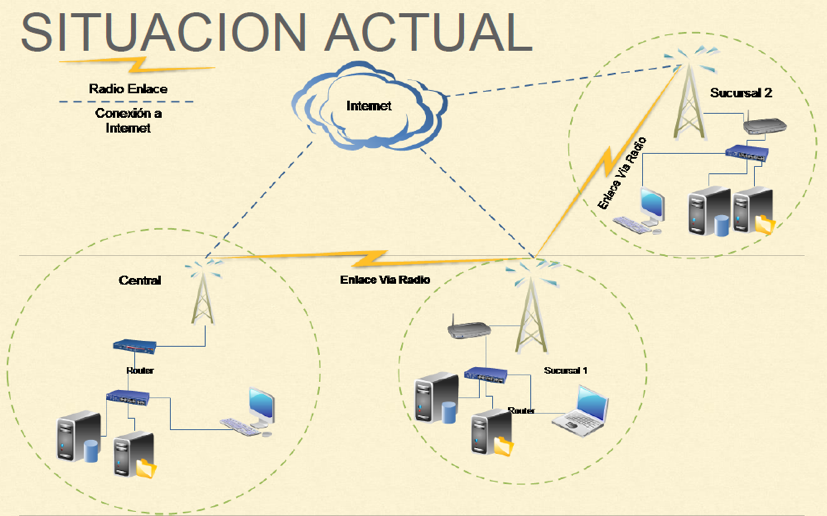
\includegraphics[scale = .8]{figuras/figura003.png}
\caption{Situacion Actual, donde cada filial tiene un servidor para cada servicio.}
\label{situacion-actual}
\end{center}
\end{figure}
Una vez realizado la conexi�n por medio de tuneles redundates, como se puede ver en la (Fig. \ref{situacion-esperada}), los datos quedan almacenado en el servidor de la central, de esta manera reducir al minino los problemas de incoherencia a causas de replicaciones.\\
\begin{figure}[H]
\begin{center}
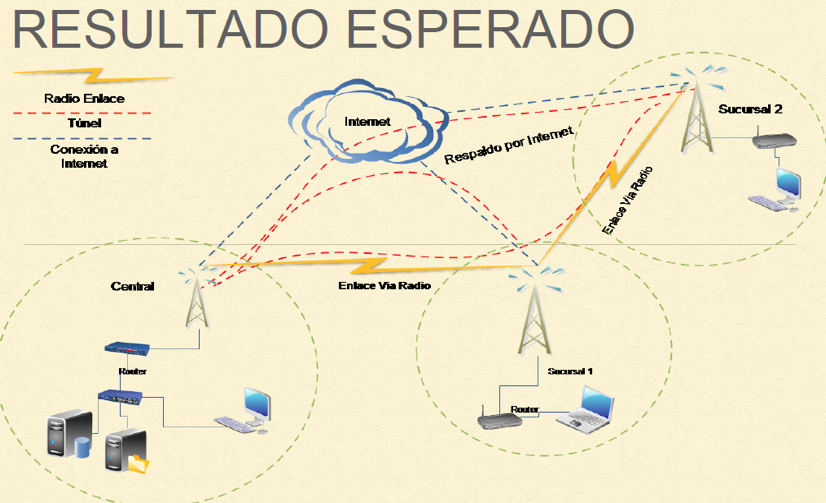
\includegraphics[scale = .8]{figuras/figura004.png}
\caption{Situacion Esperada, con la implementacion de los tuneles redundates, los servidores quedan centalizados.}
\label{situacion-esperada}
\end{center}
\end{figure}
\subsection{Pregunta General}
?`Cu�l es la manera para conectar sucursales con la central a trav�s de VPNs?
\subsection{Preguntas Espec�ficas}
?`Cu�l es el modelo de infraestructura que responde de manera m�s eficiente para la centralizaci�n de datos utilizando VPN?\\
?`Cu�les son los equipos hardware y software a ser utilizado para la implementaci�n de la centralizaci�n de datos a trav�s de VPN? \\
?`Qu� cantidad de recursos humanos ser�n necesarios y cu�l ser� el orden de desarrollo del trabajo para la implementaci�n de la centralizaci�n de datos a trav�s de VPN? \\
?`Cu�les son las recomendaciones para tener una seguridad m�nima en la centralizaci�n de los datos a trav�s de VPN?

\section{Antecedentes}
La importancia de la tecnolog�a de las redes de datos para las comunicaciones en las organizaciones (empresas, instituciones gubernamentales, no gubernamentales) ha sido fundamental para su desarrollo y crecimiento, tanto en el aspecto econ�mico y funcional, siendo una herramienta estrat�gica que brinda soporte y permite el desenvolvimiento y transformaci�n de dichas organizaciones. Hoy en d�a no se puede concebir, a nivel organizacional, alg�n cambio, fusi�n u uni�n sin considerar las comunicaciones y las tecnolog�as de informaci�n que le dan soporte.\\
Ya se realizaron varios trabajos relacionados a \Gls{vpn}, cada una de ellas con sus particularidades. 
Cabe destacar \textit{``Redes VPNs de Acceso Remoto''}, realizado por Mario Rub�n Mansilla y Eduardo Rodolfo Colombres, donde los objetivos generales fueron: Investigar las caracter�sticas, componentes, mecanismos de una VPN de acceso remoto y como solucionan la necesidad de un ingreso seguro a los recursos inform�ticos de la organizaci�n desde cualquier sitio y Aplicar los conceptos de VPN de acceso remoto a trav�s de una soluci�n que implemente un cliente VPN port�til que evite la instalaci�n de programas para esta tarea.\cite{red:vpn}
\textit{``Las comunicaciones en las redes privadas virtuales''} de Jes�s y Juan Hern�ndez donde el objetivo principal es implementar VPN en una plataforma Windows.\cite{protocolo:2003}
En otro trabajo similar, \textit{``Estudio e implementaci�n de un radio enlace con tecnolog�a mikrotik para el ISP Sistemas en el cant�n gualaquiza, provincia morona santiago''}, de Klever Mauricio Suqui Carchipulla . Estos autores estudian las propiedades de los radios enlaces a profundidad.\cite{suqui:2010}
\fancyhead{}
\fancyfoot{}


\lhead{Radiofrecuencia, su historia, sus protocolos de se�alizaci�n}

\chapter{RadioFrecuencia}

\section{Marco Te�rico}
Es de sobra conocido que vivimos en la era de la informaci�n. Este hecho tiene unas connotaciones inmediatas que tambi�n son conocidas universalmente. La primera de ellas es que en la sociedad actual la informaci�n tiene un gran valor, es m�s, en muchas ocasiones la informaci�n es el propio ``valor'' o, al menos, la informaci�n es el valor que marca la diferencia. \\
Muchas empresas y organizaciones, solo gestionan y negocian con informaci�n. Para ellas, la informaci�n es el �nico activo y, por lo tanto, el m�s valioso. Como tal elemento de valor, la informaci�n debe ser custodiada con el m�ximo cuidado porque, sin lugar a duda, ser� buscada por otros. \cite{gutierrez:2003}\\
Hoy en d�a as� como han crecido potencialmente las tecnolog�as, la masificaci�n del uso de Internet y el uso de aplicaciones en red, tambi�n han crecido las amenazas inform�ticas, las cuales pueden provocar desde una infecci�n en la computadora con virus hasta interrumpir completamente la funcionalidad de un sistema empresarial.\cite{sanchez:2012}\\
A fin de garantizar la seguridad de este bien de las empresas u organizaciones, es imprescindible protegerla, de forma a que se evite las p�rdidas por eventos accidentales o intencionales.\\

Entre los t�rminos de seguridad dentro del �mbito de las Tics, se pueden definir los siguientes:\\
\begin{itemize}
	\item Amenaza es un evento que puede desencadenar un incidente en la organizaci�n propietaria, produciendo da�os materiales o perdidas inmateriales en sus activos.
	\item Activos son recursos para que la organizaci�n funcione correctamente con el fin de alcanzar sus objetivos propuestos. En el caso que nos compete, el activo principal es la informaci�n y los activos secundarios son los propios sistemas inform�ticos (hardware). 
	\item Vulnerabilidad es la posibilidad de ocurrencia de la materializaci�n de una amenaza sobre un activo.
	\item Impacto es la consecuencia sobre un activo de la materializaci�n de una amenaza sobre el activo.
	\item Riesgo es la probabilidad de que se produzca un impacto determinado en un activo de la organizaci�n.\cite{seguridad:2013}
\end{itemize}

Desde del inicio de las telecomunicaciones, cuando una informaci�n es transmitida por un canal de comunicaci�n est� sometida a riesgos porque existe amenazas y el canal de comunicaci�n tiene vulnerabilidades (un canal de comunicaci�n es, en la mayor�a de los casos, esencialmente inseguro e inestable).\cite{seguridad:2004}\\

\subsection{Radiofrecuencia} 
Cuando hablamos de radio, la mayor�a de la gente piensa en la radio FM, que usa una frecuencia de alrededor de 100 MHz. Entre la radio y el infrarrojo encontramos la regi�n de las microondas con frecuencias de 1 GHz a 300 GHz, y longitudes de onda de 30 cm a 1 mm.\\
Las frecuencias m�s importantes para nosotros son las de 2 400 - 2 495 MHz, usadas por los est�ndares 802.11b y 802.11g (correspondientes a longitudes de onda de alrededor de 12.5 cm), y las de 5.150 - 5.850 GHz (correspondientes a longitudes de onda de alrededor de 5 a 6 cm), usadas por 802.11a. El est�ndar 802.11n puede trabajar en cualquiera de estas bandas. en la (Fig. \ref{espectro-electromagnetico}) nos muestra el uso de cada frecuencia.

\begin{figure}[H]
\begin{center}
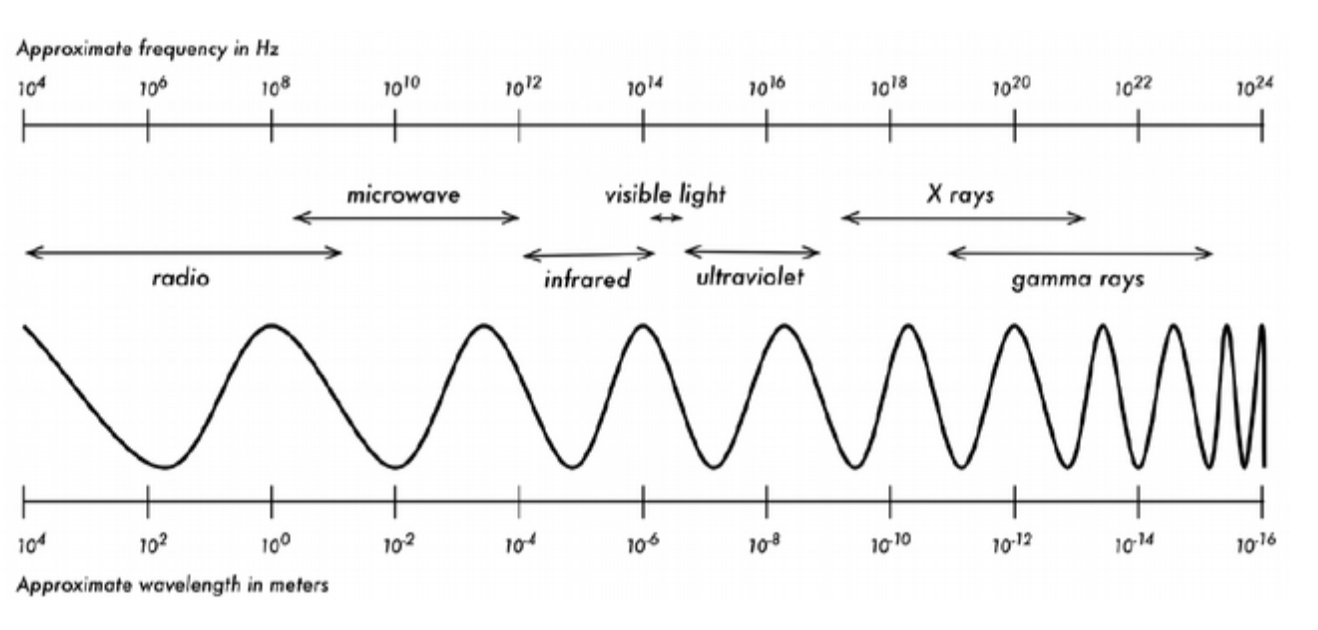
\includegraphics[scale = .5]{figuras/figura005.png}
\caption{Escala del espectro electromagn�tico \cite{wireless:desarrollo}}
\label{espectro-electromagnetico}
\end{center}
\end{figure}
\subsection{Ancho de Banda}
Un t�rmino que vamos a encontrar a menudo en la f�sica de radio es ancho de banda. El ancho de banda es simplemente una medida de rango de frecuencia. Si un dispositivo usa el rango de 2.40 GHz a 2.48 GHz, decimos que el ancho de banda ser�a 0.08 GHz (es decir 80 MHz).
Se puede ver f�cilmente que el ancho de banda que defnimos aqu� esta muy relacionado con la cantidad de datos que se pueden trasmitir a mayor cantidad de frecuencias disponibles, mayor cantidad de datos se pueden transmitir en un momento dado. El t�rmino ancho de banda es a menudo utilizado para algo que deber�amos m�s bien denominar tasa de transmisi�n de datos, por ejemplo ``mi conexi�n a Internet tiene 1 Mbps de ancho de banda'', lo que signifca que �sta puede trasmitir datos a 1 megabit por segundo.\cite{wireless:desarrollo}

\subsection{Ondas Electromagn�ticas}
La forma de propagaci�n de las ondas electromagn�ticas se genera por la aceleraci�n de una carga el�ctrica. Estas viajan a una velocidad cercana a los 300.000 km/s, sin embargo cuando esta viaja a trav�s de la materia las velocidades que alcanza son mucho menores, a mayor densidad menor velocidad.\cite{wireless:desarrollo}\\
La radiaci�n electromagn�tica se propaga por el universo como ondas interactivas de campos el�ctricos y magn�ticos; y se puede ordenar en un espectro que va desde ondas de frecuencias elevadas hasta ondas con frecuencia muy bajas.\\
Existe una divisi�n del espectro de frecuencias que fue establecida por el Consejo Consultivo Internacional de las Comunicaciones de Radio (\Gls{CCIR}) en el a�o 1953.\cite{ccir:1927}\\


\subsection{Polarizaci�n} 
Es aquel fen�meno que se produce cuando el campo el�ctrico oscila solo en un plano determinado, denominado plano de polarizaci�n. Este plano puede definirse por dos vectores, uno de ellos paralelo a la direcci�n de propagaci�n de la onda y otro perpendicular a esa misma direcci�n el mismo que indica la direcci�n del campo el�ctrico.

\subsection{Tipos de Polarizaci�n}
Como se describi� anteriormente la polarizaci�n est� definida por la trayectoria que describe el campo el�ctrico o magn�tico sobre un plano, en funci�n de esto la polarizaci�n se clasifica en: polarizaci�n lineal, circular, el�ptica. En el siguiente grafico se ilustra de mejor manera dicha clasificaci�n, en donde el campo el�ctrico est� representado por el color azul, los componentes X, Y por el color rojo y verde, el eje vertical representa el tiempo, y el color purpura es la trayectoria que describe el vector en el plano.
\begin{figure}[htb]
\begin{center}
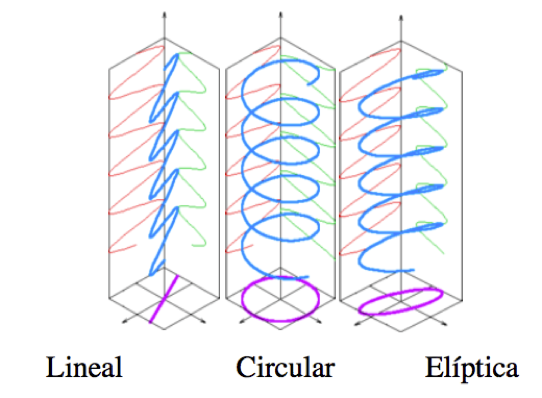
\includegraphics[scale = .9]{figuras/figura006.png}
\caption{Tipos de Polarizaci�n \cite{suqui:2010}}
\label{tipos-polarizacion}
\end{center}
\end{figure}
\subsection{Usos de la Polarizaci�n}
Cada vez que se realiza un radioenlace, necesitamos el uso de antemas para conseguir un mayor alcance para la se�al a emitir, sin embargo, en el momento de instalarlas nos encontramos con la posibilidad de elegir entre una polarizaci�n horizontal o vertical, la diferencia est� pr�cticamente que cuando se alineada verticalmente (el trozo de alambre recto), los electrones solo se mueven de arriba a abajo, no hacia los lados (porque no hay lugar hacia donde moverse) y por consiguiente los campos el�ctricos solo apuntan hacia arriba o hacia abajo verticalmente. El campo que abandona el alambre y viaja como una onda tiene una polarizaci�n estrictamente lineal (y en este caso vertical). Por otra parte la polarizaci�n horizontal tendremos un movimiento de los electrones de izquierda a derecha, por lo tanto el campo que abandona el alambre viaja como una onda con polarizaci�n lineal horizontal.
Cabe se�alar que cuando se alinean dos antenas, as� consigamos los mejores niveles de se�al, y si estas no se encuentran polarizadas correctamente, no podremos transmitir informaci�n por el enlace
\subsection{Caracter�sticas fundamentales de las ondas de radio}
El comportamiento de las ondas depender� del medio de transmisi�n, del tipo de informaci�n que se desee enviar, y de los equipos a utilizar. En resumen las caracter�sticas principales de las ondas de radio son:
\begin{itemize}
	\item La distancia que pueden llegar a recorrer, ya que depender� de la potencia del equipo transmisor.
	\item La cantidad de informaci�n que se podr� transmitir, esto depender� de la cantidad de ondas que puedan entrar en un periodo de un segundo (frecuencia). Cuanto m�s r�pida sea la oscilaci�n o ciclo de la onda, mayor cantidad de informaci�n puede transportar.
	\item Cuanto m�s corta sea la onda m�s alta ser� su frecuencia.
	\item Las ondas con longitudes de onda m�s larga tienden a viajar m�s lejos que las que tienen longitudes de onda m�s cortas.
	\item Las ondas m�s largas rodean los obst�culos. La distancia que una onda puede viajar depende de la relaci�n entre la longitud de onda de la misma y el tama�o de los obst�culos en su camino de propagaci�n.
\end{itemize}
\subsection{Reflexi�n Y Refracci�n De Ondas}
Si bien es cierto las ondas electromagn�ticas pueden viajar en el vac�o, pero por lo general estas se propagan por un medio que puede ser el�stico u homog�neo. Cuando las ondas viajan a trav�s de un medio inicial, su trayectoria se ve afectada, produci�ndose as� los efectos conocidos como reflexi�n, refracci�n y dispersi�n de ondas.

\subsection{Reflexi�n y Transmisi�n}
Cuando una onda viaja, y esta se encuentra con otro tipo de superficie, la mayor parte de la onda incidente que se refleja sobre dicha superficie se conoce como reflexi�n. La reflexi�n puede ser de dos tipos: especular cuando la superficie de incidencia es lisa (el �ngulo de incidencia es igual al reflejado), y difusa cuando la superficie de incidencia tiene imperfecciones. La reflexi�n y transmisi�n de perturbaciones oscilatorias es com�n tanto a las ondas mec�nicas como a la luz y ondas electromagn�ticas.\\
Las dos leyes que resumen el fen�meno de la reflexi�n con respecto al medio de separaci�n son:
\begin{enumerate}[(I)] 
 \item Cada rayo de la onda incidente y el rayo correspondiente de la onda reflejada est�n contenidos en un mismo plano, que es perpendicular a la superficie de separaci�n entre los dos medios en el punto de incidencia.
 \item El �ngulo que forman el rayo incidente y el rayo reflejado con la recta perpendicular a la frontera son iguales. Estos �ngulos se conocen, respectivamente, como �ngulo de incidencia y �ngulo de reflexi�n. Es decir, los rayos incidentes y reflejados se encuentran en el mismo plano, que es perpendicular al de incidencia, y forman un mismo �ngulo con la normal en el punto de incidencia.
\end{enumerate}
\begin{figure}[htb]
\begin{center}
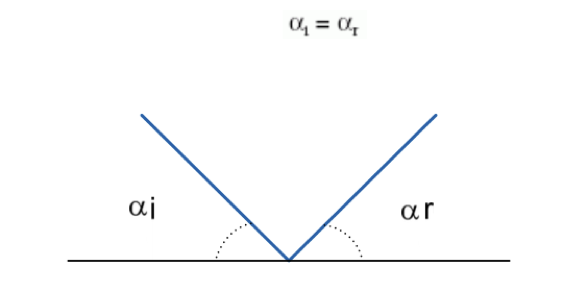
\includegraphics[scale = .9]{figuras/figura007.png}
\caption{Rayo incidente y reflejado \cite{suqui:2010}}
\label{incidente-reflejado }
\end{center}
\end{figure}
\subsection{Refracci�n}
Durante la transmisi�n de una onda cuando esta se encuentra con un segundo medio, parte de la onda se refleja, y resto es absorbida por el segundo medio (onda refractada), a este fen�meno se conoce con el nombre de refracci�n, resumiendo tenemos que la refracci�n se rige por dos leyes principales:
\begin{enumerate}[(I)] 
 \item Cada rayo de la onda incidente y el rayo correspondiente de la onda refractada forman un plano que es perpendicular a la superficie de separaci�n entre los medios en el punto de incidencia.
\item El �ngulo que forma el rayo refractado con la normal, llamado �ngulo de refracci�n, est� relacionado con el �ngulo de incidencia por una formula denominada ley de Snell, (1580-1626). Expresada matem�ticamente esta ley indica que: los rayos incidentes y refractados est�n situados en un mismo plano, que es perpendicular al de la superficie de separaci�n entre los medios. Los �ngulos que determinan la direcci�n de propagaci�n guardan entre s� una relaci�n regida por la ley de Snell.\cite{ley:snell}
\end{enumerate}
\begin{figure}[htb]
\begin{center}
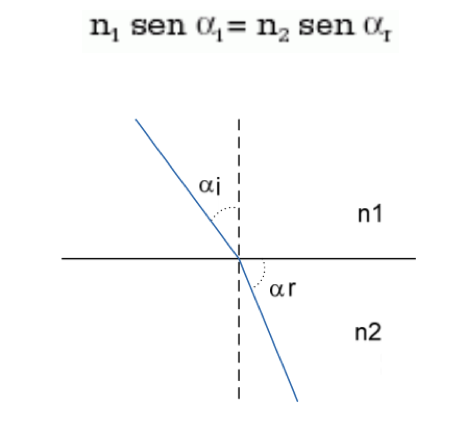
\includegraphics[scale = .9]{figuras/figura008.png}
\caption{Rayo incidente y refractado \cite{suqui:2010}}
\label{incidente-refractado }
\end{center}
\end{figure}
\subsection{Dispersi�n}
La velocidad de la luz en un medio dado depende de la longitud de onda. De este modo, al incidir sobre una superficie de separaci�n con un mismo �ngulo de incidencia, se refracta con un �ngulo de refracci�n diferente para cada longitud de onda (y, por tanto, para cada frecuencia, que determina el color). As�, si se hace incidir un haz de luz blanca sobre una superficie de separaci�n, cada color de la luz se refracta con un �ngulo diferente, para formar un efecto de arco iris. Este fen�meno se denomina dispersi�n de la luz.

\subsection{Difracci�n}
Difracci�n es el comportamiento de las ondas cuando al incidir en un objeto dan la impresi�n de doblarse. Es el efecto de ?`ondas doblando las esquinas?. Imagine una onda en el agua viajando en un frente de onda plana, tal como una ola llegando a una playa oce�nica. Ahora ponemos en su camino una barrera s�lida, como una cerca de madera, para bloquearla. Luego practicamos una estrecha rendija en esa pared, como una peque�a puerta. Desde esta abertura va a comenzar una onda circular, y por supuesto va a alcanzar puntos que est�n en una l�nea directa detr�s de esa abertura, pero tambi�n a ambos lados de ella. Si miramos este frente de onda, y pudiera ser tambi�n una onda electromagn�tica, como un haz de luz, ser�a dif�cil explicar c�mo logra alcanzar puntos que est�n ocultos por una barrera. Este fen�meno se puede apreciar mejor en la siguiente figura:
\begin{figure}[htb]
\begin{center}
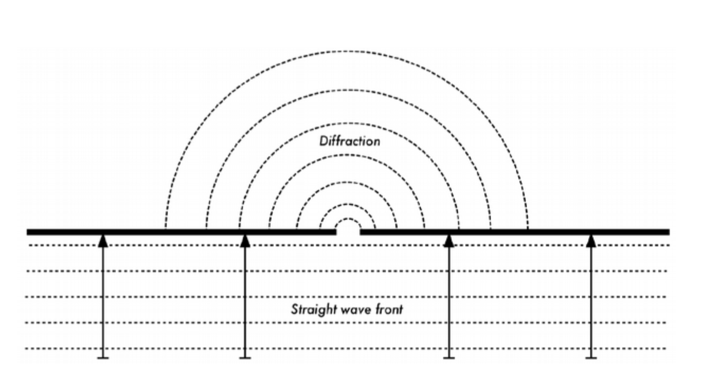
\includegraphics[scale = .9]{figuras/figura009.png}
\caption{Difracci�n a trav�s de una ranura peque�a \cite{wireless:desarrollo}}
\label{difraccion}
\end{center}
\end{figure}

Se debe tener en cuenta que en la difracci�n se genera una p�rdida de potencia, la potencia de la onda difractada es significativamente menor que el frente de onda que la provoca. Pero en algunas aplicaciones muy espec�ficas, se puede aprovechar el efecto de difracci�n para rodear obst�culos.
Interferencia de ondas electromagn�ticas\\
Es fen�meno se produce cuando dos ondas de la misma frecuencia avanzan m�s o menos en la misma direcci�n y tienen una diferencia de fase que permanece constante en el transcurso del tiempo, pueden combinarse de tal manera que su energ�a no se distribuye uniformemente en el espacio, sino que es m�xima en ciertos puntos y m�nima en otros 
\begin{figure}[htb]
\begin{center}
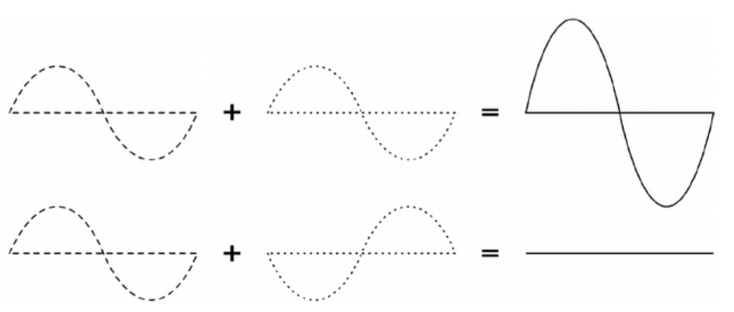
\includegraphics[scale = .9]{figuras/figura010.png}
\caption{Interferencia de ondas: constructiva (izquierda) y destructiva (derecha)\cite{wireless:desarrollo}}
\label{constructiva-destructiva}
\end{center}
\end{figure}
Los m�ltiples sistemas radio el�ctricos existentes en nuestro medio operan sobre un �nico rango de frecuencias, y para poder tener acceso a �l es necesario obtener un permiso previo de la entidad encargada de administrar el espectro en cada pa�s. Los sistemas radioel�ctricos actuales pueden soportar varias interfaces permitiendo incorporar diferentes equipos de radioenlaces a una red ya instalada. La informaci�n de un sistema de radioenlaces se difunde desde un transmisor hacia un receptor por medio de una frecuencia fija.
\begin{figure}[htb]
\begin{center}
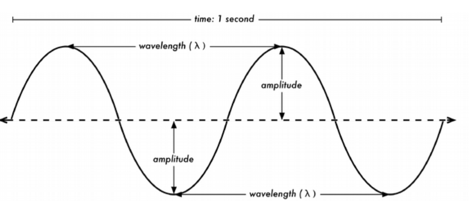
\includegraphics[scale = .9]{figuras/figura011.png}
\caption{Longitud de onda, amplitud, y frecuencia \cite{wireless:desarrollo}}
\label{amplitud-frecuencia}
\end{center}
\end{figure}
\subsection{Transmisi�n y Recepci�n}
Para conseguir la propagaci�n de las ondas electromagn�ticas, se sigue todo un proceso que inicia en el emisor cuya funci�n es la de producir una onda portadora, en donde caracter�sticas son modificadas dependiendo del tipo de se�al a transmitir, una vez que se ha propagado la onda a trav�s de una frecuencia fija, el receptor capta la onda y la desmodula con el fin de obtener as� la se�al original.

En el sistema de modulaci�n de amplitud (\Gls{am}), la se�al (de baja frecuencia) se superpone a la amplitud de ondas hertzianas portadora (de alta frecuencia). En el sistema de modulaci�n de frecuencia (\Gls{fm}), la amplitud de la onda portadora se mantiene constante, pero la frecuencia var�a seg�n la cadencia de las se�ales moduladoras. Este sistema permite eliminar par�sitos e interferencias, y reproduce el sonido con mayor fidelidad.

\subsection{Usos de la radiofrecuencia}
Originalmente los sistemas de radiofrecuencia se utilizaron para la comunicaci�n naval, hoy en d�a, este t�rmino abarca muchas m�s aplicaciones entre las cuales se incluye las redes inal�mbricas, comunicaciones m�viles de todo tipo, y la radiodifusi�n.
A continuaci�n describiremos m�s detalladamente en que aplicaciones se usa los sistemas de radio frecuencia.

\begin{itemize}
\item Audio
\begin{itemize}
	\item Transmisi�n voz y servicios interactivos con el sistema de radio Digital
	\item Servicios civiles y militares en alta frecuencia (HF) en la banda de Onda Corta, para comunicaci�n con barcos en alta mar y con poblaciones o instalaciones aisladas y a muy largas distancias.
	\item Sistemas telef�nicos celulares digitales para uso cerrado (polic�a, defensa, ambulancias, etc.) Distinto de los servicios p�blicos de telefon�a m�vil.
\end{itemize}
\item Telefon�a
\item Video
\item Navegaci�n
\item Servicios de emergencia
\item Transmisi�n de datos por radio digital
\end{itemize}
\subsection{Caracter�sticas y tipos de enlaces}
Una vez conocido como se propaga las ondas en nuestro medio, debemos tener en cuenta algunas caracter�sticas con respecto a un enlace inal�mbrico, desde que es, como funciona, y hasta los factores que debemos considerar para establecer un enlace.

\subsection{Propagaci�n radioel�ctrica}
La propagaci�n a trav�s del espacio depender�s de la superficie de la tierra, su forma y su constituci�n (mar, tierra cultivada, desierto, etc.), y la atm�sfera, tanto la troposfera como la ionosfera.
\begin{figure}[htb]
\begin{center}
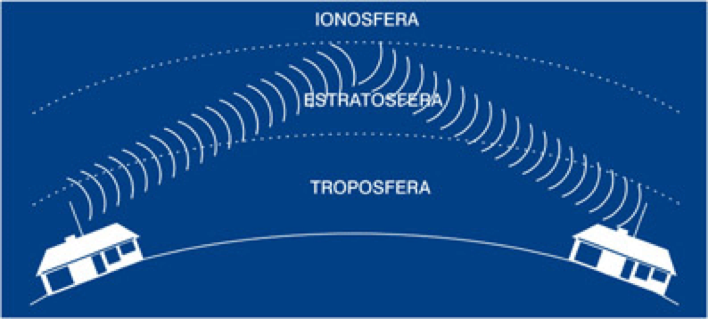
\includegraphics[scale = .9]{figuras/figura012.png}
\caption{Propagaci�n de las ondas sobre la superficie terrestre \cite{propa:onda}}
\label{ondas-superficie}
\end{center}
\end{figure}

Cuando la se�al se transmite esta viaja en todas direcciones, aunque la energ�a sigue la curvatura de la tierra, es decir que la propagaci�n est� relacionada directamente con la banda de frecuencia en la que se trabaja.
\begin{itemize}
	\item En frecuencias inferiores a 30 \Gls{khz}, existe un mecanismo de propagaci�n por gu�a-ondas tierra ionosfera.
	\item En frecuencias desde 10KHz y hasta 3 \Gls{mhz} el principal mecanismo de propagaci�n utilizado es la onda de superficie.
	\item En frecuencias por encima de 3 MHz (1 MHz) y hasta unos 30 MHz el mecanismo fundamentalmente utilizado es la onda ionosf�rica. Por reflexi�n ionosf�rica se consiguen enlaces de hasta 4000 Km en un solo salto, y m�s por m�ltiples reflexiones ionosfera tierra (mar).
	\item En frecuencias por encima de unos 30 MHz, el principal mecanismo es la onda espacial. Debido a la curvatura de la superficie terrestre, a partir del horizonte el mecanismo posible de propagaci�n son las ondas difractadas, que a estas frecuencias tienen alcances muy peque�os.
	\item A partir de 40 o 50 MHz la ionosfera no refleja las ondas electromagn�ticas por lo que puede utilizarse para comunicaciones extraterrestres.
\end{itemize}
\subsection{Sistemas de radiocomunicaciones inal�mbricas}
La comunicaci�n inal�mbrica inicio con la postulaci�n de las ondas electromagn�ticas por James Clerk Maxwell (1860), la demostraci�n de la existencia de estas ondas fueron confirmadas por Heinrich Rudolf Hertz (1880), y con la invenci�n del tel�grafo inal�mbrico por Guillermo Marconi. Pero no fue sino hasta el a�o de 1896 en donde se concedi� la primera patente de comunicaciones inal�mbricas a Guillermo Marconi en el Reino Unido. Desde aquel momento, entonces el n�mero de desarrollos en el campo de las comunicaciones inal�mbricas tomaron ese sitio. La comunicaci�n inal�mbrica fue un suceso novedoso y muy importante ya que este permiti� cruzar barreras a la que las conexiones guiadas nos manten�an atadas, especialmente por las distancias que se pod�a conseguir con estas.\cite{radio:2009}\\
Un enlace inal�mbrico es aquel que no necesita de un medio guiado para la transmisi�n de informaci�n, este presenta grandes ventajas frente a la conexi�n por cable, ya que su instalaci�n puede llegar a lugares geogr�ficos imposible para una red cableada, con la facilidad de transportar datos y voz. En la actualidad las redes inal�mbricas ofrecen igual o hasta mejor confiablidad, calidad y velocidad en comparaci�n con algunas conexiones de Internet v�a sat�lite, estos enlaces se realizan desde un punto donde exista la posibilidad de contratar un acceso a Internet hasta el punto donde sea necesaria dicha conexi�n.

\subsection{L�nea de vista directa}
El t�rmino l�nea vista, a menudo abreviada como LOS (por su sigla en ingl�s, Line of Sight), es f�cil de comprender cuando se habla acerca de la luz visible, si podemos ver un punto B desde un punto A donde estamos, tenemos l�nea de vista directa. La l�nea visual que necesitamos para tener una conexi�n inal�mbrica optima desde un punto A hasta otro B, es m�s que simplemente una l�nea delgada, su forma es m�s bien la de un cigarro, un elipsoide. Su ancho puede ser descrito por medio del concepto de zonas de Fresnel.

\subsection{La Zona de Fresnel}
La teor�a exacta de las zonas de Fresnel es algo complicada. Sin embargo el concepto es f�cilmente entendible, se sabe por el principio de Huygens que por cada punto de un frente de onda comienzan nuevas ondas circulares, por ende se sabe que los haces de microondas se ensanchan. Tambi�n que las ondas de una frecuencia pueden interferir unas con otras. La teor�a de zona de Fresnel simplemente examina a la l�nea desde A hasta B y luego al espacio alrededor de esa l�nea que contribuye a lo que est� llegando al punto B. Algunas ondas viajan directamente desde A hasta B, mientras que otras lo hacen en trayectorias indirectas. Consecuentemente, su camino es m�s largo, introduciendo un desplazamiento de fase entre los rayos directos e indirectos. Siempre que el desplazamiento de fase es de una longitud de onda completa, se obtiene una interferencia constructiva, las se�ales se suman �ptimamente. Tomando este enfoque, y haciendo los c�lculos, se encuentra con que hay zonas anulares alrededor de la l�nea directa de A hacia B que contribuyen a que la se�al llegue al punto B. Se debe tener en cuenta que existen muchas zonas de Fresnel, pero para este caso interesa principalmente la zona 1. Si �sta fuera bloqueada por un obst�culo, por ejemplo un �rbol o un edificio, la se�al que llegue al destino lejano ser� atenuada. Entonces, cuando se planea enlaces inal�mbricos, se debe estar seguro de que esta zona va estar� libre de obst�culos. En la pr�ctica de redes inal�mbricas ya se puede trabajar con que al menos el 60 por ciento de la primera zona de Fresnel est� libre.\cite{ipvideo:2014}\\
\begin{figure}[htb]
\begin{center}
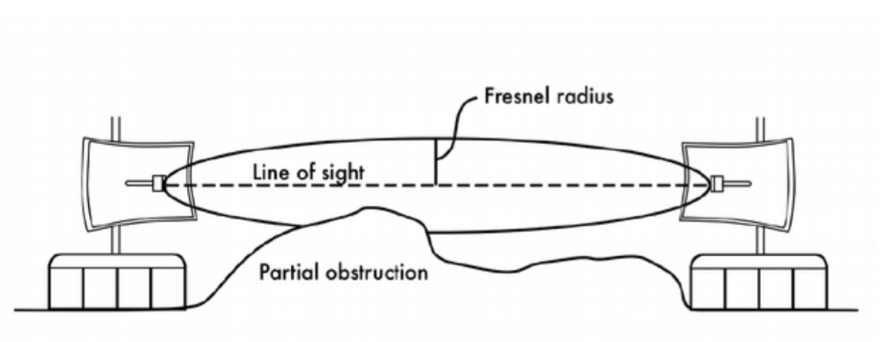
\includegraphics[scale = .9]{figuras/figura013.png}
\caption{La zona de Fresnel est� bloqueada parcialmente en este enlace aunque la l�nea visual (line of sight) no est� obstruida \cite{wireless:desarrolo}}
\label{zona-fresnel}
\end{center}
\end{figure}
La siguiente ecuaci�n es la f�rmula para calcular la primera zona de Fresnel:\\
\begin{equation}
r=17.31*\sqrt{(((d1*d2)/( f*d)))}
\end{equation}

Donde r es el radio de la primera zona en metros, d1 y d2 son las distancias desde el obst�culo a los extremos del enlace en metros, d es la distancia total del enlace en metros, y f es la frecuencia en MHz. Note que esta f�rmula calcula el radio de la zona. Para calcular la altura sobre el terreno, debe sustraerse este resultado de una l�nea trazada directamente entre la cima de las dos torres.

\subsection{Energ�a}
La potencia P es clave para lograr que los enlaces inal�mbricos funcionen, se necesita cierto m�nimo de potencia para que el receptor le d� sentido a la se�al. Ahora vamos a discutir brevemente c�mo se define y calcula la potencia P. El campo el�ctrico se mide en \Gls{v/m} , la potencia contenida en �l es proporcional al campo el�ctrico al cuadrado, expresado en la ecuaci�n.

\begin{equation}
P \approx E^2
\end{equation}
En la pr�ctica, se mide la potencia por medio de alg�n tipo de receptor, por ejemplo una antena y un volt�metro, un medidor de potencia, un osciloscopio, o inclusive una tarjeta inal�mbrica y una computadora port�til. La potencia es proporcional al cuadrado del voltaje de la se�al.

\subsection{C�lculo en dBs}
La t�cnica sin duda m�s importante para calcular la potencia es por decibeles (\gls{db}). No hay f�sica nueva en esto, es solamente un m�todo conveniente que hace que los c�lculos sean muy simples. El decibel es una unidad sin dimensi�n, es decir, define la relaci�n entre dos medidas de potencia. Se define como en la ecuaci�n:

\begin{equation}
dB = 10 * log(P1/P0)
\end{equation}

Donde $P1$ y $P0$ pueden ser de los dos valores cualesquiera que se quiere comparar. T�picamente, en este caso, se tratar� de potencia.\\
Aqu� hay algunos valores utilizados com�nmente que es importante recordar:\\
\begin{itemize}
\item +3 dB = doble potencia
\item -3 dB = potencia media
\item +10 dB = orden de magnitud (10 veces la potencia)
\item -10 dB = un d�cimo de potencia
\end{itemize}
Adem�s de los dBs a dimensionales, hay cierto n�mero de definiciones relacionadas que est�n basadas en una referencia P0 fija. Los m�s relevantes para nosotros son:\\
\begin{itemize}
\item dBm relativo a P0 = 1 mW
\item dBi relativo a una antena isotr�pica ideal
\end{itemize}
Una antena isotr�pica es una antena hipot�tica que distribuye uniformemente la potencia en todas direcciones. La antena que m�s se aproxima a este concepto es el dipolo, pero una antena isotr�pica perfecta no puede ser construida en la realidad. El modelo isotr�pico es �til para describir la ganancia de potencia relativa de una antena real.
\subsection{Ventajas de un enlace inal�mbrico}
A continuaci�n se da a conocer algunas ventajas de este tipo de redes permitiendo comprender cu�l es su alcance real.
\begin{itemize}
	\item Accesibilidad: en la actualidad existen equipos que permiten enlazar zonas geogr�ficas imposibles de llegar con una red cableada, o que simplemente resultar�a costoso, permitiendo a un usuario final tener acceso a esta red, siempre y cuando se encuentre dentro del �rea de cobertura, lugar en donde se encuentran los equipos de difusi�n.
	\item Movilidad: especialmente para los usuarios que disponen de una l�nea celular, permiti�ndoles acceder a la red, cuando este en movimiento y desde cualquier lugar siempre y cuando este en un lugar en donde haya cobertura.
	\item Productividad: El poder tener acceso a la informaci�n permite disminuir la brecha digital existente en algunos sectores. El Internet en la actualidad es una herramienta fundamental en cada negocio, porque esta no solo permite establecer una comunicaci�n, sino que tambi�n la mayor�a de transacciones se las hace a trav�s del internet.
	\item F�cil Instalaci�n: El hecho de no utilizar un medio guiado, la instalaci�n se la puede realizar en un tiempo m�s corto, y por ende resultar� m�s rentable.
	\item Escalabilidad: A medida que una empresa crece, necesita tambi�n ampliar su cobertura, como es el caso de los I.S.P. que generalmente su �rea de cobertura no se ve limitado, y conforme crecen pueden expandirse a otros sectores, con solo establecer el nuevo punto de enlace para poder llegar con el servicio al usuario que lo necesite.
	\item Seguridad: Las instalaciones inal�mbricas son f�ciles de monitorear, y por ende poseen seguridades s�lidas, permitiendo �nicamente al personal capacitado, poder acceder a estas.
	\item Costos: Con una red inal�mbrica se puede reducir los costes, ya que se eliminan o se reducen los costes de cableado durante los traslados configuraciones o expansiones.
\end{itemize}
\subsection{Estructura de un radio enlace}
Un radio enlace est� constituido por estaciones terminales y repetidoras intermedias, con equipos transceptores, antenas y elementos de supervisi�n y reserva. Adem�s de las estaciones repetidoras, existen las estaciones nodales donde se desmodula la se�al y de la baja a banda base y en ocasiones se extraen o se insertan canales. Al tramo terminal estaci�n nodal se lo denomina secci�n de conmutaci�n y es una entidad de control, protecci�n y supervisi�n.
En cuanto a los repetidores se los puede clasificar en activos o pasivos.
\begin{itemize}
	\item Activos: En ellos se recibe la se�al en la frecuencia de portadora y se la baja a una frecuencia intermedia (FI) para amplificarla y retransmitirla en la frecuencia de salida. No hay demodulaci�n y son transceptores.
	\item Pasivos: Se comportan como espejos que reflejan la se�al y se los puede dividir en pasivos convencionales, que son una pantalla reflectora y los pasivos back-back, que est�n constituidos por dos antenas espalda a espalda. Se los utiliza en ciertos casos para salvar obst�culos aislados y de corta distancia.
\end{itemize}
Los enlaces son estructuralmente sistemas en serie, de tal manera que si uno falla se pierde la comunicaci�n a trav�s de la red. Por ello se le exige los equipos en cada nodo posean una alta disponibilidad y confiabilidad Esto tambi�n implica que utilicen sistemas de supervisi�n y control de alto rendimiento para detectar f�cilmente una falla en el sistema.
Conceptos de dise�o
Como se mencion� anteriormente la forma de garantizar el correcto funcionamiento del enlace es necesario que entre dos puntos a conectar exista l�nea de vista directa, es decir que entre el enlace exista una altura libre de obst�culos para la adecuada propagaci�n en toda �poca del a�o, tomando en cuenta las variaciones de las condiciones atmosf�ricas de la regi�n. Para poder calcular las alturas libres debe conocerse la topograf�a del terreno, as� como la altura y ubicaci�n de los obst�culos que puedan existir en el trayecto.
El dise�o de un radio enlace se puede resumir en los siguientes pasos:
\begin{itemize}
	\item Definir el modo de transmisi�n, es decir en condiciones de visibilidad directa, este puede ser punto a punto o transmisi�n omnidireccional.
	\item Tener en cuenta los diferentes factores que pueden degradar nuestra se�al como por ejemplo el ruido.
	\item El alcance deseado depender� especialmente de la potencia de los equipos a transmitir.
	\item Tener en cuenta bajo qu� condiciones se producir� las p�rdidas o atenuaci�n de la se�al.
\end{itemize}
Una vez analizado la parte t�cnica, para la implementaci�n del enlace se debe considerar:
\begin{itemize}
	\item Elecci�n del sitio de instalaci�n.
	\item Relevamiento del perfil del terreno y c�lculo de la altura del m�stil para la antena.
	\item C�lculo completo del radio enlace, estudio de la trayectoria del mismo y los efectos a los que se encuentra expuesto.
	\item Prueba posterior a la instalaci�n del radio enlace, y su posterior puesta en servicio con tr�fico real.
\end{itemize}
\subsection{Enlaces Punto - Punto}
Las redes punto a punto son aquellas que responden a un tipo de arquitectura de red en las que cada canal de datos se usa para comunicar �nicamente dos nodos. En una red punto a punto, los dispositivos en red act�an como socios iguales, o pares entre s�. Los enlaces que interconectan los nodos de una red punto a punto se pueden clasificar en tres tipos seg�n el sentido de las comunicaciones que transportan:
\begin{itemize}
	\item Simplex: La transacci�n s�lo se efect�a en un solo sentido.
	\item Half-d�plex: La transacci�n se realiza en ambos sentidos, pero de forma alternativa, es decir solo uno puede transmitir en un momento dado, no pudiendo transmitir los dos al mismo tiempo.
	\item Full-D�plex: La transacci�n se puede llevar a cabo en ambos sentidos simult�neamente.\end{itemize}
Cuando la velocidad de los enlaces Semi-d�plex y D�plex es la misma en ambos sentidos, se dice que es un enlace sim�trico, en caso contrario se dice que es un enlace asim�trico. 
\begin{figure}[htb]
\begin{center}
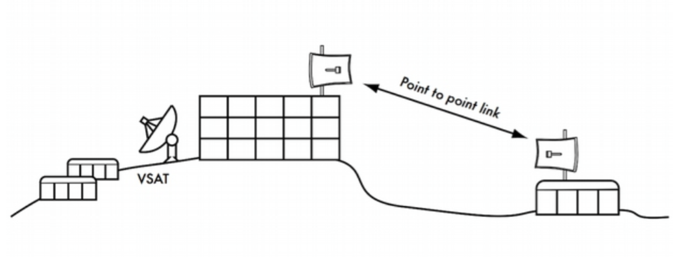
\includegraphics[scale = .9]{figuras/figura014.png}
\caption{Enlace Punto - Punto \cite{wireless:desarrollo}}
\label{punto-punto}
\end{center}
\end{figure}
Los enlaces punto - punto pueden conseguir un mayor alcance utilizando antenas de grilla o plato tanto en el receptor como en el transmisor, permitiendo expandir a una red de forma f�cil y r�pida. La velocidad de transferencia conseguida con estos tipos de enlaces tiene un promedio 20Mbytes, sin ninguna dificultad.

\subsection{Enlaces Punto - Multipunto}
El enlace punto a multipunto es la versi�n del punto a punto para la conexi�n r�pida y fiable de m�s de dos instalaciones. Para reducir costes, este sistema consta de una instalaci�n central dotada de una antena multidireccional, a la que apuntan las antenas direccionales del resto de centros. Esto permite una capacidad igual a la del punto a punto, pero extensible hasta a 16 centros.
\begin{figure}[htb]
\begin{center}
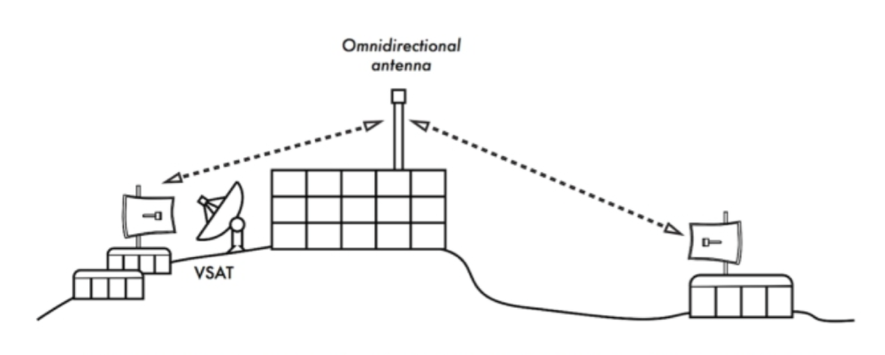
\includegraphics[scale = .9]{figuras/figura015.png}
\caption{Enlace Punto Multipunto \cite{wireless:desarrolo}}
\label{enlace-punto-multipunto}
\end{center}
\end{figure}
Algunas de las aplicaciones de este tipo de redes permiten:
\begin{itemize}
	\item Mantener una constante comunicaci�n con las diferentes sucursales de una empresa, permiti�ndome compartir base de datos, acceso, etc.
	\item Implementar redes de voz sobre IP, permiti�ndome reducir costos de llamadas entre sucursales.
	\item Venta de acceso a Internet (I.S.P.).
	\item Monitoreo a trav�s de c�maras de vigilancia.
\end{itemize}
\subsection{Conexi�n De Rejilla O Malla}
La siguiente configuraci�n es una consecuencia de las dos anteriores usada especialmente en redes inal�mbricas privadas. Es configuraci�n conocida como rejilla o malla en donde cada punto o nodo puede trasmitir a cualquier otro que est� disponible o accesible. Esta configuraci�n es muy flexible ya que permite a un nodo trasmitir a otro v�a cualquier otro nodo.
\begin{figure}[htb]
\begin{center}
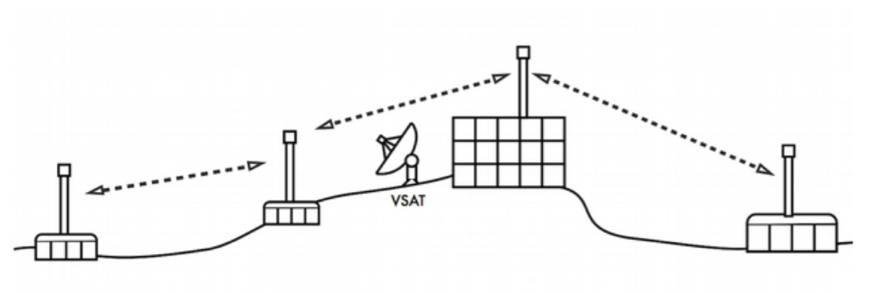
\includegraphics[scale = .9]{figuras/figura016.png}
\caption{Conexi�n Malla \cite{wireless:desarrollo}}
\label{conexion-malla}
\end{center}
\end{figure}
\subsection{Distribuci�n De Acceso Inal�mbrico (HotSpot)}
La distribuci�n HotSpot, no es un tipo de enlace, sino m�s bien parte de uno. El HotSpot consiste en puntos de conexi�n en zonas p�blicas o privadas como aeropuertos, parques, institutos educativos, restaurantes, etc., permitiendo que el usuario que disponga de un equipo WIFI acceda al internet banda ancha. Los HotSpots permiten que el acceso inal�mbrico sea una realidad mucho m�s compleja y extensible que el Internet que hoy se conoce. No se trata solo de estar en un lugar f�sicamente y poder conectarte a la Red sin el cable, es mucho m�s. El concepto lleva a que Internet, la oficina, la empresa, se va con el usuario, por lo que se puede arriesgar a pensar en una incursi�n similar a la del m�vil.

\subsection{Sistemas de microondas}
El control de tr�fico a�reo, navegaci�n marina, control de misiles, aviaci�n, telecomunicaciones, son algunas de las aplicaciones de las microondas, en la actualidad las frecuencias de microondas son utilizadas cada vez m�s en telecomunicaciones, cuando se utilizan antenas repetidoras, necesarias a lo largo de un camino o trayecto de comunicaci�n. Las microondas comprenden frecuencias que trabajan en el rango de los 109 a 1012 Hertz, que corresponden a longitudes de onda que van de los 30 cm. (cent�metros) a 0.3 mm. (Mil�metros). Estas longitudes de onda son del mismo orden de magnitud que las dimensiones de los circuitos empleados en su generaci�n. La transmisi�n en un sistema de microondas se utiliza para cubrir distancias mayores, el receptor recibe la se�al enviada por un transmisor en una frecuencia inicial, la convierte a sus propiedades el�ctricas y la retransmite a otra estaci�n de microonda, en algunos casos puede hacerlo cambiando de frecuencia para retransmitir.\cite{sistema:micro}
\subsection{Radiocomunicaciones por sat�lite}
Podemos definir a la comunicaci�n por sat�lite como: ``un repetidor radioel�ctrico ubicado en el espacio, recibe se�ales generadas en la tierra, las amplifica y las vuelve a enviar a la tierra''. Un sat�lite ofrece grandes ventajas con respecto a otros sistemas, entre los m�s importantes est� mayor potencia de transmisi�n y mayor �rea de cobertura. La transmisi�n por sat�lite se ha utilizado com�nmente en nuestro medio, para comunicaciones de larga distancia, y comunicaciones internacionales transatl�nticas. Pero el elevado costo que implica el disponer de una estaci�n terrestre, equipos electr�nicos para la conexi�n satelital, ocasionan que el usuario opte por otro medio de comunicaci�n como la microonda, fibra �pticas, radioenlaces, etc., cuyos costos de instalaci�n son mucho menores cada d�a, mientras que los costos para un enlace satelital se mantienen siempre elevados. Con los sistemas por sat�lite se dispone de gran cantidad de ancho de banda puesto que el espectro de frecuencias puede asignarse a una base de acceso fijo o bajo demanda. Puesto que la se�al se debe transmitir al sat�lite situado a 22300 millas, el costo de alquiler de un canal no es sensible a la distancia, por lo que las ventajas que presentan los sat�lites en el momento de transmisi�n, pesan m�s que los inconvenientes que ocasionan.\\
Con respecto a las desventajas, cabe citar el elevad�simo costo inicial, el cual solo podr�a ser afrontado mediante la gesti�n de grandes emprendimientos, aunque puede considerarse que no constituye obst�culo insalvable, sino que el principal inconveniente estar�a dado en la necesidad de tomar una decisi�n pol�tica a trav�s de la cual, se superen intereses sectoriales y contradictorios en lo que ata�e a este tema, y se implemente definitivamente el sistema teniendo en miras fundamentalmente el bien de toda la comunidad.\cite{comunicacion:satelite}
\subsection{Red Privada}
Las redes de datos interconectaban, en un principio en forma local, las computadoras personales de una organizaci�n, permitiendo compartir la informaci�n, y el trabajo en grupo de una forma m�s �gil y eficiente. Sin embargo esto requiri� considerar el aspecto de la seguridad, ya que si bien se trabajaba en un mismo �mbito, es decir dentro de la misma empresa, no todos los usuarios deb�an acceder a los datos por igual. Este esquema funcion� para peque�as organizaciones, pero para aquellas cuyas estructuras, incluida sitios geogr�ficamente alejados, surgi� la necesidad de interconectar tambi�n dichos lugares.\\

La soluci�n vino de la mano de los proveedores de servicio de red de �rea amplia de datos o \Gls{wan}, a trav�s de la contrataci�n de enlaces dedicados, los cuales conectaban las redes distantes con la red central. Esta soluci�n implicaba un costo, que result� prohibitivo para la mayor�a, excepto para aquellos que pod�an abonar un costo fijo de contrataci�n m�s un valor que variaba proporcionalmente a la distancia existente entre los sitios a interconectar (mile-age fee). En la actualidad existen tecnolog�as WAN (Frame Relay, ATM) donde el costo est� en funci�n del caudal de datos o ancho de banda comprometido del enlace, que una organizaci�n est� dispuesta a pagar, sin considerar ya la distancia geogr�fica. De esta forma se cuenta con una red privada o estructura de comunicaci�n propia, en el sentido de que el control y la administraci�n de la red est�n bajo el dominio de la organizaci�n. Las pol�ticas de uso, los servicios suministrados, los medios activos y pasivos de comunicaci�n por donde fluyen los datos est�n bajo un control propio. Si bien las comunicaciones de �rea amplia son suministradas por un proveedor, este se compromete a respetar los requerimientos de la organizaci�n cliente, adem�s, los datos que atraviesan su red, no estar�n al alcance de otros clientes.
\subsection{Red P�blica}
Uno de los eventos m�s importantes que acompa�� al desarrollo de las redes en las organizaciones, fue la r�pida evoluci�n de la mayor de las redes IP existentes, Internet. Esta se define como un sistema cooperativo de interconexi�n de redes que suministra un servicio de comunicaci�n universal. De esta manera satisface la necesidad de los usuarios de comunicar dos puntos cualesquiera, tambi�n denominados sistemas o nodos finales, pudiendo acceder a recursos m�s all� de los disponibles en un �nico sistema y ubicados fuera de los l�mites de la red local. Los datos atraviesan redes intermedias hasta llegar a su destino, en una operaci�n no orientada a la conexi�n, mediante el uso de equipos especiales denominados routers, tambi�n conocidos como sistemas o nodos intermedios. La naturaleza no orientada a la conexi�n de Internet, significa que no hay una ruta preestablecida o circuito virtual dedicado entre los sistemas que se comunican, tampoco niveles de servicio, priorizaci�n o separaci�n de tr�fico que puedan aplicarse a los datos que se transmiten.\\
La funci�n de los routers es interconectar al menos dos redes, transfiriendo paquetes desde una red a otra. Estas pertenecen a diversas organizaciones y proveedores. Esto convierte a Internet en una red p�blica, en el sentido de que son muchos los que participan en su conformaci�n y los medios de transmisi�n son compartidos. Depender� de quien utilice la infraestructura de Internet para comunicar dos sistemas finales, tomar las medidas de seguridad apropiadas para asegurar la confidencialidad, autenticidad, integridad y no repudio de los datos transmitidos.\cite{red:vpn}
\subsection{Red Privada Virtual}
El funcionamiento de algunas organizaciones, determinaron la necesidad de permitir el acceso a la red propia a usuarios que se encontraban geogr�ficamente fuera de los l�mites de �sta. �stos requer�an desplazarse con frecuencia y en alg�n momento acceder a sus archivos en la red local, revisar su correo electr�nico o utilizar un sistema de informaci�n. En un principio se utilizaron servicios de acceso remoto mediante la implementaci�n de servidores para tal fin o RAS (Remote Access Server), el uso de l�neas discadas para la conexi�n y pools de m�dems para atender las llamadas. Toda esta infraestructura era costeada por la organizaci�n la cual era responsable de su administraci�n y mantenimiento. Si bien se solucionaba el problema de acceso a la red local, se lograba a un costo econ�micamente alto.\\
Otra necesidad fue la de encontrar una alternativa m�s econ�mica de interconectar diversas redes entre s� y ya no solamente las de una misma organizaci�n, sino redes de diferentes organizaciones. Razones de pol�tica estrat�gica justificaban este desaf�o, ya sea a nivel empresarial, universitario o gubernamental. Ambos requerimientos tuvieron su soluci�n a partir de la idea de utilizar Internet, teniendo en cuenta su alcance global y su capacidad de entrega de datos a casi cualquier sistema final a un bajo costo. Dado que se utiliza Internet para transmitir datos, no hay garant�a de que estos no puedan ser captados por terceros. Tambi�n es claro que los sistemas finales que se comunican est�n expuestos.\\
En la actualidad no solo se considera a Internet como medio donde una organizaci�n puede implementar una VPN. Los proveedores de servicios de comunicaciones o SP (Service Provider) ofrecen servicios de VPN de acuerdo a las necesidades del cliente a trav�s de su red backbone. Un SP puede administrar m�ltiples VPNs pertenecientes a varios clientes operando a trav�s de su backbone.



\fancyhead{}
\fancyfoot{}


\lhead{VPN - Definici�n - Tipos}

\chapter{Definici�n de VPN}
Es habitual encontrar varias definiciones sobre VPN, aunque �stas no difieren en esencia. Algunas de ellas pueden ser:
\begin{itemize}
	\item ``Una VPN es una red privada construida dentro de una infraestructura de red p�blica, como la red Internet''
	\item ``La idea b�sica de una VPN es muy simple. Una corporaci�n podr�a tener un n�mero de oficinas (o grupos de ellas) en diferentes lugares, y en cada uno de estos tener su propia red local. Muchas corporaciones han aumentado la cantidad de empleados que deben trabajar en forma remota, ya sea desde sus hogares o en forma itinerante. Interconectar estas redes y lugares mediante una red compartida (no privada) crea una VPN''
	\item ``Una red privada virtual basada en Internet utiliza la infraestructura abierta y distribuida de Internet para transmitir datos entre sitios corporativos'' 
	\item ``Una red privada virtual es una red privada de datos que utiliza una infraestructura de telecomunicaci�n p�blica, manteniendo la privacidad mediante protocolos de t�nel y procedimientos seguros. El prop�sito principal de una VPN es dar a la compa��a la misma capacidad que otorgan los enlaces dedicados contratados pero a un costo menor, utilizando medios de comunicaci�n p�blicos.'' 
\end{itemize}
Se puede definir a una VPN de manera m�s formal. Esta definici�n aparece publicada en el art�culo \textit{What Is a VPN? Part 1} escrito por Ferguson y Houston para la publicaci�n mensual The Internet Protocol Journal de Cisco System en Marzo de 2001:
\textit{``Una VPN es un ambiente de comunicaciones en el cual existe un control de acceso, para permitir la conexi�n entre sistemas pares �nicamente dentro de una comunidad de inter�s definida, y est� creado considerando alguna forma de partici�n de un medio de comunicaci�n subyacente, donde este brinda servicios a la red de una forma no exclusiva.''}
De acuerdo a estas definiciones se puede decir que una red privada virtual es una red, que comunica dos o m�s dispositivos finales (estos a su vez pueden interconectar una red completa) que pueden estar ubicados geogr�ficamente distantes y representan una comunidad de inter�s. Para esto se utiliza como medio de transmisi�n una estructura compartida com�n a varios usuarios. �sta puede ser Internet o la red principal o backbone de un proveedor de servicios de comunicaciones.\\
Se dice privada porque los dispositivos que no participan en esta comunicaci�n no tienen acceso al contenido de la misma y de hecho no son conscientes de su establecimiento. El acceso a esta red y su administraci�n est� restringido solo a un n�mero limitado de dispositivos. La privacidad se aplica tambi�n al espacio de direccionamiento y esquema de enrutamiento utilizado en una VPN, en el sentido de que est�n separados o difieren de aquellos instrumentados en alguna otra red privada existente o en la infraestructura de red subyacente por donde ocurre la comunicaci�n.\\
El concepto de virtual, por definici�n es la representaci�n de un objeto no existente mediante la ejecuci�n de funciones que simulan su existencia. En el contexto de una VPN, significa que esta �ltima representa una red de comunicaciones, que no tiene una contraparte f�sica real. Este concepto fundamenta la naturaleza discreta o de separaci�n, de una red l�gica privada funcionando sobre una infraestructura de comunicaciones compartida y real. El aspecto de privacidad, definido en el p�rrafo anterior, est� en funci�n de la virtualizaci�n.\cite{what:2001}
\section{Terminolog�a}
La literatura relacionada con redes privadas virtuales est� llena de acr�nimos, siglas, t�rminos muy espec�ficos que tornan dif�cil la interpretaci�n de cualquier lectura relacionada con el tema. Esta secci�n define los principales elementos que componen un escenario VPN.
\begin{itemize}
	\item Sitio: ubicaci�n geogr�fica con uno o m�s usuarios o uno o m�s servidores o una combinaci�n de servidores y usuarios. El usuario refiere al host o estaci�n de trabajo.
	\item Servidor VPN: software o firmware VPN el cual se ejecuta en un dispositivo. Tiene la funci�n de establecer un t�nel con un cliente VPN. Previamente verifica la identidad del cliente para autorizar su acceso y determinar los permisos de este para acceder a los recursos locales. El dispositivo donde se ejecuta el servidor VPN puede ser un host, router o switch. Este equipo comunica la red local con la red p�blica. Otras acepciones pueden ser: gateway VPN, servidor de t�neles.
	\item Cliente VPN: software o firmware VPN ejecut�ndose en un dispositivo, cuya funci�n es establecer un t�nel con un servidor VPN. Previamente, debe presentar las credenciales correctas al servidor. Otra acepci�n puede ser cliente de t�nel.
	\item T�nel: Enlace l�gico entre el servidor y cliente VPN, creado por un protocolo de t�nel. Por este canal se env�an los datos que han sido encapsulados y quiz�s encriptados por el protocolo. Es posible transmitir datos sin encriptar por un t�nel. Un t�nel puede establecerse en diferentes capas del modelo ISO/OSI de protocolos de comunicaciones.
	\item Extremos de un t�nel: dispositivos que gestionan la creaci�n, el establecimiento y la finalizaci�n de un t�nel mediante la ejecuci�n de software o firmware dedicado para tal fin, por lo tanto se encargan tambi�n del procesamiento relacionado con la des/encapsulaci�n, des/encriptaci�n y transmisi�n de los paquetes recibidos.
	\item \Gls{nas} : servidor de acceso de red, un dispositivo que representa una interface entre un medio de acceso como la red de telefon�a y una red de conmutaci�n de paquetes, como el backbone de un proveedor o Internet. En una VPN este dispositivo permite que un usuario utilizando un acceso telef�nico acceda a su red mediante un t�nel creado por el NAS hacia el servidor de acceso remoto de la red destino.
	\item T�nel voluntario (Voluntary Tunnel): T�nel creado y configurado a partir de la solicitud de un cliente VPN. Esta clase de t�nel es com�n en las VPN de acceso remoto, donde uno de los extremos es una computadora personal o notebook de un usuario hogare�o o m�vil.
	\item T�nel obligatorio (Compulsory Tunnel): T�nel asociado con las VPN de acceso remoto. Su creaci�n y configuraci�n est� a cargo de un dispositivo denominado servidor de acceso de red o NAS. �ste se ubica entre la PC del usuario y el servidor VPN. En el NAS se ubica el extremo del t�nel donde funciona el cliente VPN. Es posible que m�ltiples usuarios conectados al servidor de acceso de red, compartan el t�nel en forma concurrente. En general el NAS es propiedad y es administrado por un proveedor de servicios.
	\item Dispositivo de borde: Es el dispositivo ubicado en la frontera entre la red local y la red p�blica.
	\item CE: Dispositivo de borde del cliente (Customer Edge Device). Es el equipo perteneciente a un cliente de un servicio de comunicaciones que se sit�a en el borde de la red privada local y conecta con la red del proveedor del servicio a trav�s de un PE. Un CE puede ser un router o switch.
	\item C: Dispositivo que pertenece al cliente y que se ubica dentro de la red del mismo. Estos no tienen conectividad directa con la red del Proveedor ni participan de la VPN. Pueden ser routers o switchs.
	\item PE: Dispositivo de borde del proveedor (Provider Edge Device). Este es propiedad del proveedor de servicio de comunicaciones. Se conecta directamente a la red del cliente a trav�s del CE. Un PE puede ser un router, switch o un dispositivo que combine ambas funciones.
	\item P: Dispositivos que componen el n�cleo de la red del Proveedor. No tienen conectividad directa con la red del cliente ni participan de las VPN. Estos son equipos como routers y switches.
\end{itemize}
\begin{figure}[H]
\begin{center}
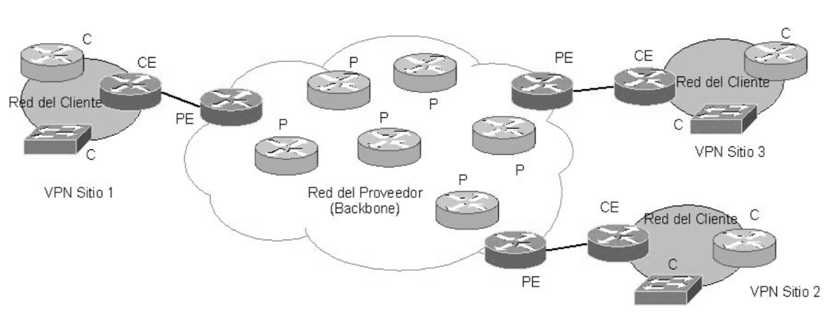
\includegraphics[scale = .9]{figuras/figura017.png}
\caption{Componentes de una VPN \cite{red:vpn}}
\label{componet-vpn}
\end{center}
\end{figure}
\subsection{Clasificaci�n}
Se pueden encontrar varias clasificaciones de las VPN, lo cual puede generar cierta confusi�n. Esto se debe a que existen diversos tipos de tecnolog�as y clases de redes privadas virtuales, lo que permite m�s de un criterio de organizaci�n.
Las clasificaciones generales y m�s habituales son:
\begin{itemize}
\item De acuerdo a quien implementa y administra el servicio: la propia organizaci�n o un proveedor de servicios.
\item Seg�n que comunican: redes entre s� o usuarios a la red.
\item Seg�n la capa del modelo de referencia de pila ISO/OSI para comunicaciones donde se establece la VPN: capa 2, 3 y las VPNs de capa de aplicaci�n/transporte que utilizan el protocolo \Gls{ssl/tls}. Estas representan una clase particular de VPN que se describen aparte.\cite{ssl:2011}
\end{itemize}
Otros criterios pueden ser:
\begin{itemize}
\item Seg�n si los dispositivos de borde de un proveedor participan o no en el enrutamiento del tr�fico de datos del cliente: VPN peer to peer o VPN overlay.
\item Seg�n si son orientadas o no a la conexi�n.
\item Si son confiables o seguras.
\end{itemize}
\subsection{VPNs provistas por el cliente o por el proveedor}
Uno de los principales criterios para clasificar las VPN, define quien est� a cargo de la implementaci�n y administraci�n de la red privada virtual, ya sea el cliente (la organizaci�n) o el proveedor de servicios de comunicaciones. Esto se refiere a la definici�n de las pol�ticas a cumplir con esta soluci�n, los requerimientos para la implementaci�n, la adquisici�n y configuraci�n de equipamiento, mantenimiento, resoluci�n de problemas y monitoreo, especificaci�n del espacio de direccionamiento a utilizar, esquema de enrutamiento etc.
\subsection{VPNS provistas por el cliente (CE o CPE VPN)}
Tambi�n denominadas VPNs del �mbito del cliente (Customer Promises VPN). Estas VPNs son definidas e implementadas por el cliente de un servicio de comunicaciones. Generalmente este tiene acceso al backbone de un proveedor o bien posee un servicio de acceso a Internet. En este contexto el cliente puede tener m�s de un sitio propio, geogr�ficamente distante que desea conectar o bien requiere hacerlo con otra red fuera de su dominio, tambi�n remota. En este tipo de VPN, el t�nel se establece, �nicamente, entre los equipos del cliente. Estos representan los extremos del o los t�neles. Los equipos del proveedor o PE, no participan de la VPN. Tampoco del esquema de direccionamiento que esta utiliza o del enrutamiento necesario. Tratan a los paquetes o tramas como proveniente de un cliente del servicio, es decir solo lo reenv�an. En el caso de la utilizaci�n de Internet, los routers intermedios tambi�n lo hacen con los paquetes IP, sin tener en cuenta el contenido encapsulado por el t�nel de la VPN.\\
La ventaja de esta clase de VPN radica en que el cliente tiene el control de la seguridad aplicada a los datos que transmite. Para el proveedor sus dispositivos de borde no requieren ninguna configuraci�n especial para el tratamiento de los paquetes de las VPN, adem�s no surgen problemas de escalabilidad al momento de aumentar la cantidad de VPNs o los sitios a interconectar mediante estas ya que, como se mencion� anteriormente, estos equipos no participan en este escenario virtual.\\
Como desventaja, el cliente debe hacerse cargo b�sicamente de todo. Esto puede implicar un gran costo, tanto en la compra de equipamiento, como en la preparaci�n de personal para la configuraci�n y el mantenimiento de la VPN. Esta soluci�n presenta problemas de escalabilidad para el cliente cuando existen varios sitios para interconectar.

Los tipos de VPN provistas por el cliente son:
\begin{itemize}
\item VPN \Gls{ipsec} 
\item VPN \Gls{gre} 
\item VPN \Gls{ssl/tls} 
\end{itemize}
\begin{figure}[H]
\begin{center}
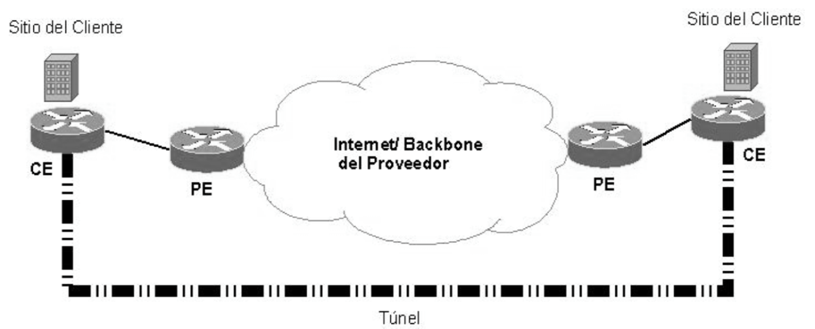
\includegraphics[scale = .9]{figuras/figura018.png}
\caption{VPN Provista por el Cliente \cite{red:vpn}}
\label{vpn-provista-cliente}
\end{center}
\end{figure}
\subsection{VPNs provistas por el Proveedor (PPVPN)}
En esta clase de VPN el proveedor de servicio se encarga de su implementaci�n. Los equipos de borde o PE participan activamente de la red virtual como as� tambi�n, pero en menor grado, los dispositivos de borde del cliente. Esto significa que los PE realizan la mayor parte del procesamiento espec�fico de la VPN, permitiendo que los equipos CE puedan ser routers o switches est�ndar sin necesidad de comprar equipamiento especial. El proveedor es responsable de la administraci�n de la VPN, liberando al cliente de estas tareas. Esto resulta, para este �ltimo, en un menor costo de implementaci�n respecto de un emprendimiento propio.
Actualmente los proveedores ofrecen un servicio de VPN mejorado, donde suman adem�s de la conectividad, acuerdos de nivel de servicio, calidad y diferenciaci�n de servicio, seguridad, ingenier�a de tr�fico, etc. Esto redunda en un producto con valor agregado que beneficia a ambas partes. Las soluciones VPN de esta clase, pueden operar en la red de un �nico proveedor, entre un conjunto de proveedores de servicio y sobre Internet. En este �ltimo caso se asume que los routers de n�cleo de Internet, no mantendr�n informaci�n referida a la VPN, sin considerar si se utilizan protocolos de enrutamiento para distribuir o no dicha informaci�n. Existen cuatro escenarios donde pueden desplegarse estas VPN6:
\begin{itemize}
\item �nico Proveedor, �nico Sistema Aut�nomo o AS (Autonomous System): escenario m�s simple, el servicio se brinda a trav�s del AS de un �nico proveedor.
\item �nico Proveedor, m�ltiples AS: un proveedor administra varios AS (adquisici�n de varias redes). Este escenario implica la distribuci�n con restricciones de la informaci�n de enrutamiento entre los diversos Sistemas Aut�nomos.
\item Multi Proveedor: es el caso m�s complejo, debido a que es necesario negociar relaciones de confianza entre los backbones de los diversos proveedores para cumplir con las medidas de seguridad y niveles de servicio acordados para la VPN de un cliente. En este caso el servicio se denomina VPN inter-AS o �nter proveedor.
\item Proveedor de Proveedores (Carrier's Carrier): este es un caso especial del primer escenario, excepto que los clientes son proveedores de servicios de comunicaciones que contratan el servicio de VPN a un proveedor principal, para ofrecerlo a su vez a sus propios clientes.
\end{itemize}
Los tipos de VPN provistas por el Proveedor son:

\begin{itemize}
\item VPN \Gls{vpws} 
\item VPN \Gls{vpls} 
\item VPN \Gls{ipls} 
\item VPN basada en routers virtuales
\item VPN IPSec
\item VPN \Gls{mpls} 
\end{itemize}
\subsection{VPNs Sitio a Sitio y de Acceso Remoto}
Otra forma general de distinguir las VPN es en funci�n de si conectan redes entre s� o usuarios a una red. Una VPN sitio a sitio (site-to- site VPN) conecta dos o m�s redes entre s� que est�n geogr�ficamente dispersas, estas pueden pertenecer a una o varias organizaciones.
Si las redes pertenecen a una misma organizaci�n, esta clase de VPN se denomina intranet. Si las redes pertenecen a varias organizaciones se conoce como extranet. La intenci�n en este �ltimo caso es comunicar organizaciones diferentes que persiguen un objetivo com�n y requieren compartir informaci�n �til para el conjunto. El servicio de VPN entre sitios deber�a ser independiente del alcance geogr�fico de la implementaci�n.
\begin{figure}[H]
\begin{center}
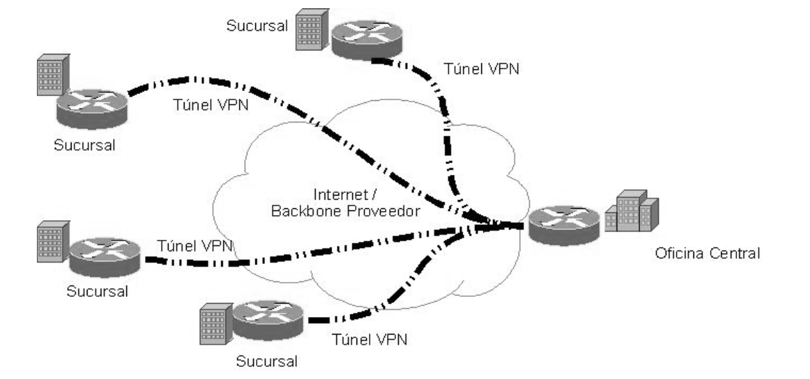
\includegraphics[scale = .9]{figuras/figura019.png}
\caption{VPN Sitio a Sitio\cite{red:vpn}}
\label{vpn-sitio-sitiol}
\end{center}
\end{figure}
Las VPN de Acceso Remoto o RAVPN (Remote Access VPN), tambi�n denominadas VPN de acceso, permiten a los usuarios m�viles o itinerantes y a los usuarios hogare�os de una organizaci�n o tele trabajadores, acceder en forma remota a la red. Esta clase de VPN puede establecer un t�nel en modo voluntario u obligatorio.
\begin{figure}[H]
\begin{center}
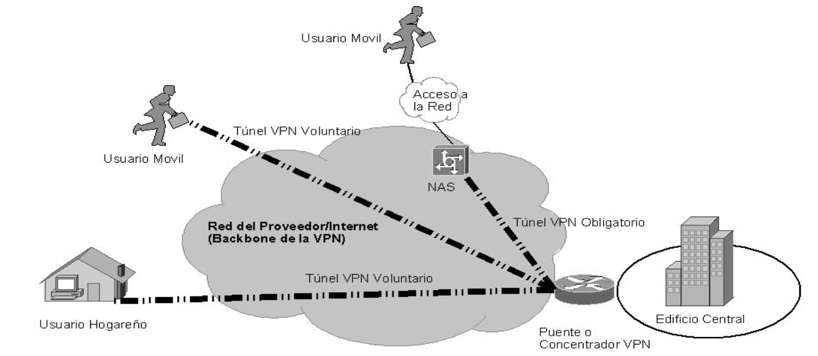
\includegraphics[scale = .9]{figuras/figura020.png}
\caption{VPN de Acceso Remoto\cite{red:vpn}}
\label{vpn-accesoremoto}
\end{center}
\end{figure}
Las tecnolog�as y protocolos asociados a esta clasificaci�n son:
VPNs sitio a sitio:

\begin{itemize}
\item IPSec
\item GRE
\item \Gls{atom} (Any Transport over MPLS)
\item \Gls{l2tpv3} (Layer 2 Tunneling Protocol version 3)
\item \Gls{ieee802q}
\item \Gls{mplslsp} (MPLS Label Switched Path)
\end{itemize}
VPNs de acceso remoto:

\begin{itemize}
\item \Gls{l2f}
\item \Gls{pptp} 
\item L2TPv2/v3
\item IPSec
\item SSL/TLS
\end{itemize}

\subsection{VPNs de capa 2 y capa 3}
El criterio de esta clasificaci�n se basa en las capas, del modelo de referencia ISO/OSI de protocolo de comunicaciones, por donde se establece el t�nel de la VPN. Esta clasificaci�n surge a partir de la variedad de tecnolog�as existentes que se utilizan para implementar la VPN.
Esta distinci�n tiene sentido cuando se la aprecia en el contexto de las clasificaciones anteriores.\\
Las VPN de capa 2 permiten la conectividad a nivel de la capa de enlace de datos y puede ser establecida entre switches, routers o hosts. La comunicaci�n est� basada en el direccionamiento de capa 2 y el reenv�o del tr�fico est� basado respecto del enlace entrante y la informaci�n de encabezados de dicha capa, tales como direcciones \Gls{mac}  o \Gls{dlci}.\\
Las VPN de capa 3 interconectan hosts o routers, la comunicaci�n se basa en el direccionamiento a nivel de capa de red. El reenv�o del tr�fico se lleva a cabo teniendo en cuenta el enlace entrante y las direcciones del encabezado IP.

\subsection{Integraci�n de las clasificaciones}
Las clasificaciones anteriores se pueden integrar para tener una perspectiva m�s pr�ctica y operativa de las VPN. Esta integraci�n muestra las VPN provista por el cliente o proveedor como el criterio de clasificaci�n m�s general, dentro de la cual se pueden diferenciar las VPN sitio a sitio y remota. Finalmente se consideran seg�n las tecnolog�as VPN de capa 2 y 3. El siguiente esquema muestra esta relaci�n:
\begin{figure}[H]
\begin{center}
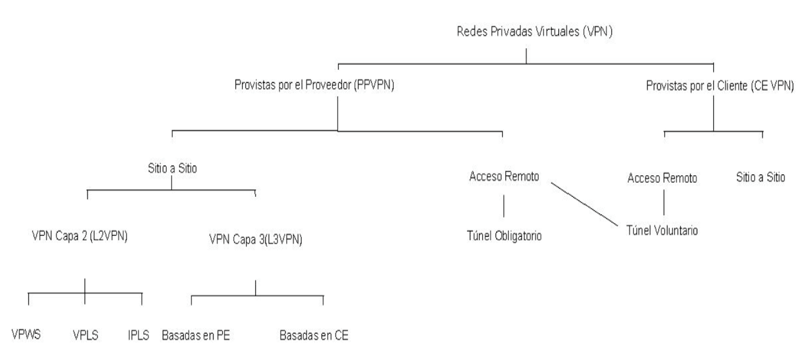
\includegraphics[scale = .9]{figuras/figura021.png}
\caption{Clasificaci�n de las VPN \cite{red:vpn}}
\label{clasifi:vpnl}
\end{center}
\end{figure}
VPN Sitio a Sitio Provistas por el Proveedor de Capa 2 (L2VPN)
Estas VPN pueden ser establecidas entre switches, routers y hosts, permitiendo la conectividad a nivel de capa de enlace entre sitios separados. Tanto el direccionamiento como el reenv�o del tr�fico de la VPN se llevan a cabo en funci�n del enlace entrante y de la informaci�n del encabezado de capa 2.
Dentro de las L2VPN se pueden distinguir dos categor�as:

\begin{itemize}
\item VPNs basadas en circuitos \Gls{p2p}: conocidas tambi�n como \Gls{vpws}. Se implementan usando MPLS o circuitos emulados (pseudowires) L2TPv3.
\item VPNs \Gls{m2m}: en esta categor�a entran las VPN \Gls{vpls} e \Gls{ipls}
\end{itemize}
\subsection{VPN VPWS}

La red del proveedor puede considerarse como una emulaci�n de un conjunto de enlaces punto a punto o pseudowires entre los sitios del cliente. Es �til en escenarios donde el cliente ya posee circuitos virtuales \Gls{atm} o Frame Relay que interconectan sus redes. En lugar de que el tr�fico del cliente atraviese el backbone hasta su destino en su formato nativo de capa 2, �ste es encapsulado y enrutado sobre la infraestructura IP del Proveedor. El cliente mantiene las conexiones de capa 2 al backbone. Los routers CE deben seleccionar el circuito virtual a usar para enviar el tr�fico al sitio destino.\\
Este esquema permite el reemplazo de redes con topolog�as estrella que requieren la interconexi�n de redes sat�lites hacia una red central, permitiendo alternativas de rutas hacia un destino. Unas de las tecnolog�as habituales, en el n�cleo de la red del proveedor, para esta clase de VPN es MPLS junto a extensiones conocidas como PWE3 (Pseudowire Emulation Edge to Edge). Un enfoque m�s escalable, respecto de la administraci�n del servicio, utiliza \Gls{bgp} (Border Gateway Protocol) como protocolo de se�alizaci�n y auto detecci�n. En este caso, los dispositivos PE usan BGP multiprotocolo para anunciar los dispositivos CE y VPN que controlan, junto con las etiquetas MPLS utilizadas para encaminar el tr�fico. De esta forma, cuando los otros CE reciben esta informaci�n, saben c�mo establecer los pseudowires.
\subsection{VPN VPLS}
En este caso la red LAN ethernet de cada sitio del cliente se extiende hasta el borde de la red backbone del proveedor. Luego, una vez all�, se emula la funci�n de un bridge o switch para conectar todas las LANs del cliente. De esta forma se emula, en la red del proveedor, una �nica LAN ethernet. Esta soluci�n provee un servicio punto a multipunto donde los routers CE env�an todo el tr�fico, destinados a los otros sitios, directamente al router PE. Este servicio se basa en la utilizaci�n de pseudowires, combinados en una topolog�a de malla completa (full mesh) de interconexiones entre los dispositivos PE que participan en una VPN determinada. �stos llevan a cabo el aprendizaje de las direcciones MAC, de la misma forma que un switch ethernet para reenviar las tramas desde un CE a otro. As�, un CE puede reenviar tr�fico en una forma punto a multipunto a otros CE. Existe un problema de escalabilidad con este servicio, y tiene que ver con el incremento de sitios del cliente. Es necesario mantener en los PE un gran n�mero de direcciones MAC para el reenv�o de tramas por sitio de cliente.

\subsection{VPN IPLS}
Si se requiere intercambiar tr�fico IP exclusivamente y los dispositivos CE son routers IP, entonces es posible el servicio IP sobre LAN. Si bien se transmiten datagramas IP, el mecanismo de reenv�o se basa en informaci�n de encabezado de capa 2. Dado que el siguiente salto o hop para cada datagrama IP es otro CE, las �nicas direcciones MAC que un PE debe aprender, cuando reenv�a las tramas de capa 2, son aquellas de los routers CE. Esto es una ventaja respecto del servicio VPLS por el reducido n�mero de direcciones MAC a preservar por sitio de cliente.

\subsection{VPN Sitio a Sitio Provistas por el Proveedor de Capa 3 (L3VPN)}
Esta clase de VPN se basa en tecnolog�as m�s estables que las empleadas en las L2VPN, debido al estudio y desarrollo de las mismas. Esto le permite al proveedor de servicio tener mayor seguridad al momento de implementar una u otra soluci�n.
Se pueden dividir a su vez en:
\begin{itemize}
\item VPN basadas en PE: Los dispositivos PE participan en el enrutamiento y reenv�o del tr�fico del cliente basado en el espacio de direcciones de la red del cliente. En este caso los CE no participan de la VPN. El tr�fico del cliente se reenv�a entre los PE a trav�s de t�neles MPLS LSP, IPSec, L2TPv3 o GRE.
\item VPN basadas en CE: En este caso los t�neles son creados entre los equipos CE, mientras los PE no participan en la VPN, solo reenv�an el tr�fico del cliente. Se utiliza IPSec o GRE para establecer los t�neles.
\end{itemize}
\subsection{Confiables y Seguras}
Esta es una clasificaci�n donde se tiene en cuenta si es o no necesaria la encriptaci�n y autenticaci�n de los datos a transferir entre los nodos de la VPN. Los proveedores que no utilizan encriptaci�n para los datos de sus clientes debido a que utilizan circuitos virtuales de capa 2 se pueden definir como VPN Confiables. Podemos mencionar las redes FRAME RELAY, ATM y MPLS. En cambio en las VPN Seguras el tr�fico de datos es autenticado y encriptado sobre el backbone del proveedor del servicio. Utilizan los protocolos IPSEC, \Gls{ssl}, L2TP asegurado mediante IPSEC, PPTP asegurado con MPPE (Microsoft Point-to-Point Encryption).

\subsection{Overlay y Peer}
Las VPN overlay se dan entre dispositivos CE, los dispositivos PE no participan en el enrutamiento de los clientes de la red, sino que reenv�an tr�fico de clientes basados en direccionamiento globalmente �nico, por lo tanto no tiene conocimiento del direccionamiento utilizado por el cliente.\\
Los t�neles son configurados entre dispositivos CE usando protocolos como IPSec y GRE. Cabe observar que el modelo overlay tiene serios problemas de escalabilidad debido a que si se cuenta con muchos nodos de egreso el n�mero de adyacencias se incrementa en directa proporci�n con el n�mero de nodos.
\begin{figure}[H]
\begin{center}
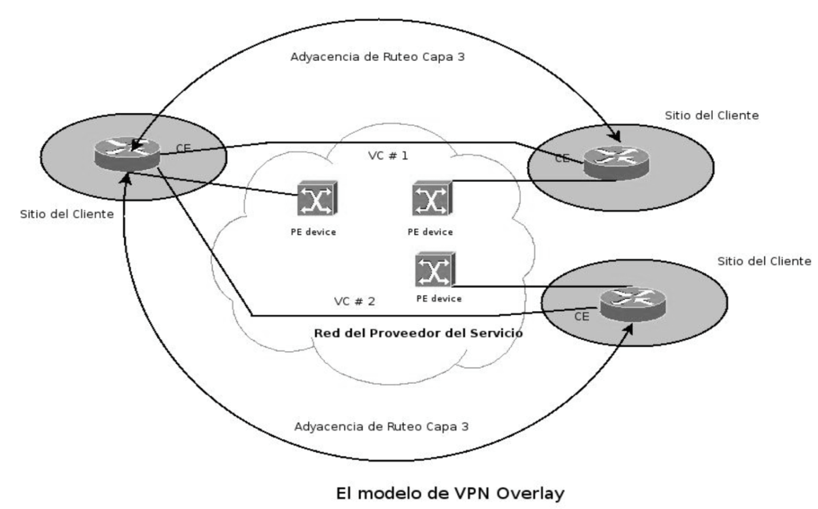
\includegraphics[scale = .9]{figuras/figura022.png}
\caption{Adyacencias del Ruteo \cite{red:vpn}}
\label{adyac:ruteo}
\end{center}
\end{figure}
Pueden ser implementadas a nivel de capa f�sica usando l�neas telef�nicas (dialup), a nivel de capa 2 utilizando Frame Relay, X-25 y ATM, o a nivel de capa 3 utilizando t�neles IP o GRE. Con el fin de clarificar veamos un ejemplo, un esquema en el que figuran tres sitios. Un sitio se conecta a trav�s de los circuitos virtuales $ VC  1� $ Y $ VC 2� $ con otros dos sitios. Si suponemos que el sitio principal es Londres y los otros son Paris y Zurich podr�amos ver que la percepci�n que poseen los routers CE 
\begin{figure}[H]
\begin{center}
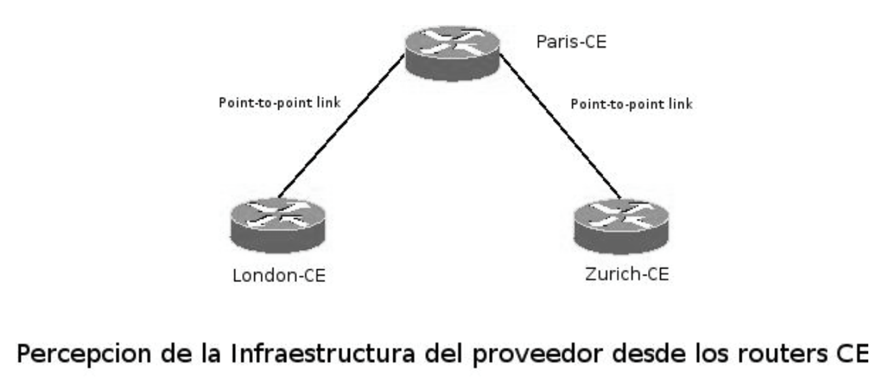
\includegraphics[scale = .9]{figuras/figura023.png}
\caption{Infraestructura del proveedor\cite{red:vpn}}
\label{infra:provee}
\end{center}
\end{figure}
Si son reemplazados los dispositivo PE por routers y estos participan en el enrutamiento entonces es una VPN tipo Peer. Los routers tienen que poseer conocimiento del direccionamiento que utiliza el cliente. Esto es necesario debido a que las rutas se intercambian entre dispositivos CE y los dispositivos PE. Estas VPN son provistas por un proveedor de servicios.
\begin{figure}[H]
\begin{center}
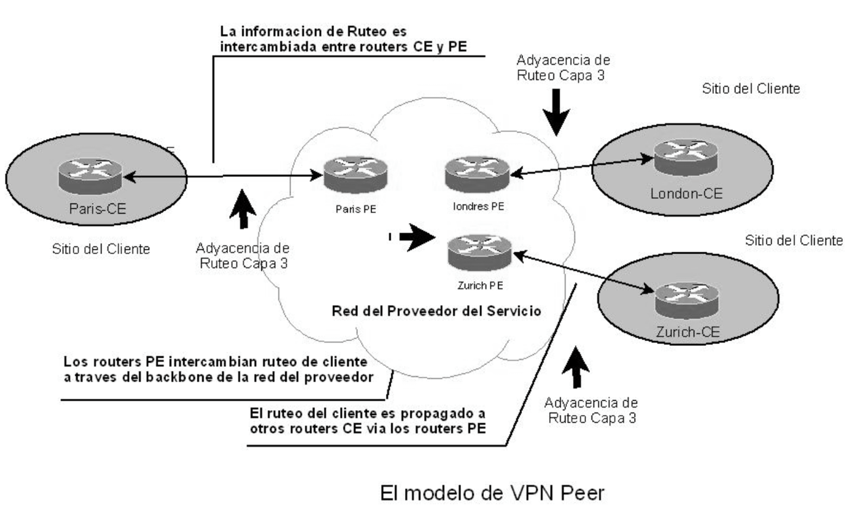
\includegraphics[scale = .9]{figuras/figura024.png}
\caption{VPNs tipo Peer\cite{red:vpn}}
\label{vpn:peer}
\end{center}
\end{figure}
En la Figura anterior podemos observar que al reemplazar los switches por routers se convierte en una VPN tipo Peer. No Orientadas y orientadas a la conexi�n\\
Son orientadas o no orientadas a la conexi�n dependiendo si el proveedor provee o no circuitos virtuales dedicados.\\
Orientada a la conexi�n: Son en las que provee el proveedor un circuito virtual dedicado. Por ejemplo FRAME RELAY y ATM.\\
No orientadas a la conexi�n: Son las que no poseen un circuito virtual. Por ejemplo las VPN basadas en IP.\\
\subsection{VPNs de capa de transporte/aplicaci�n}
El protocolo SSH (Secure Shell) desarrollado por Communications Security Ltd., permite acceder a otro dispositivo a trav�s de una red insegura, ejecutar comandos a una maquina remota y mover archivos de una computadora a otra. Utilizando encriptaci�n sobre canales inseguros provee una fuerte autenticaci�n y encriptaci�n.\\
Existen dos versiones incompatibles entre s�. Son dos protocolos totalmente diferentes que usan distinto cifrado.


\begin{table}[H]
\begin{center}
\caption{SSH v1, SSH v2}
\label{ssh-v1-ssh-v2}
\begin{tabular}{|||l|l|r||}
\hline
&SSH v1&SSH v2\\
\hline
\multirow{1}{*}{Autenticaci�n de Sistemas}&Llaves de servidor y clientes&Llaves de hosts\\
\hline
\multirow{1}{*}{Autenticaci�n}&Llaves&Certificados\\
\hline
\end{tabular}
\end{center}
\end{table}
SSH2 es una completa reescritura del protocolo que lo hace m�s seguro y utiliza una implementaci�n de red totalmente distinta que SSH1. Debido a la diferente implementaci�n ambos protocolos son incompatibles. Por ejemplo se lo utiliza para asegurar un t�nel PPP. El principio de funcionamiento es el mismo que el de SSL diferenci�ndose en la capa en la que act�an y el m�todo de autenticaci�n.
\begin{table}[H]
\begin{center}
\caption{SSH, SSL}
\label{ssh-ssl}
\begin{tabular}{|||l|l|r|||}
\hline
&SSH &SSL\\
\hline
\multirow{1}{*}{Capa en la que trabaja}&Aplicaci�n&Transporte\\
\hline
\multirow{1}{*}{Autenticaci�n}&Certificados&Llaves\\
\hline
\end{tabular}
\end{center}
\end{table}

Tambi�n es posible establecer t�neles en la capa de aplicaci�n. Para esto se utiliza un browser del lado del cliente, por lo que no es necesario instalar ning�n programa. La conexi�n se realiza a un sitio web seguro mediante el protocolo \Gls{https}. Adem�s, existen otros productos los cuales ofrecen una combinaci�n de gran flexibilidad, seguridad y que intentan lograr una configuraci�n que no requiera mucho conocimiento. La seguridad es lograda mediante cifrado del tr�fico usando el protocolo SSL/TLS.

\subsection{VPN multiservicio}
Trabajan sobre MPLS, cuyo sello distintivo es la calidad de servicio o \Gls{qos}. El objetivo de estas VPN es integrar diferentes aplicaciones en una sola conexi�n: voz, datos, multimedia, etc.

\subsection{Aplicaciones}
Las VPN se utilizan en situaciones donde es necesario establecer una comunicaci�n en forma segura utilizando un medio o infraestructura compartida de transmisi�n. Adem�s de comunicar redes propias de la organizaci�n, usuarios m�viles, tele trabajadores etc., tambi�n es posible comunicar distintas organizaciones entre s�. Esta alternativa surge a partir de la necesidad de establecer lazos de negocios, o la concreci�n de intereses comunes. La extranet refleja dichos intereses mediante la interconexi�n de las redes de datos de las distintas organizaciones. En realidad solo comparten los recursos necesarios para cumplir con los objetivos comunes, por lo que el acceso es parcial y controlado.\\
Finalmente las VPN se pueden considerar como un negocio con valor agregado en la forma de un servicio. El hecho de que hoy en d�a las organizaciones dependan fuertemente de las tecnolog�as de informaci�n para su desenvolvimiento y que sus necesidades sean diferentes, plantea un mercado donde las soluciones de comunicaciones de datos son casi a la medida del cliente. No existe una �nica soluci�n para todos los tipos de organizaciones. Es por esto que los proveedores de servicios han sumado a su oferta de soluciones empresariales, el servicio de VPN, donde una buena relaci�n costo-beneficio para el cliente es posible.
\subsection{Extranets}
Una extranet es un conjunto de intranets de organizaciones diferentes que se interconectan entre s� para cumplir con objetivos comunes. Esta relaci�n est� bien definida y es establecida bajo un estricto control del acceso. Se puede definir tambi�n como la intersecci�n de un grupo de intranets de varias empresas, lo cual indica que solo se comparte una porci�n de la intranet hacia el resto de la extranet.\\
Por otro lado Internet es el medio com�n que resuelve problemas de incompatibilidad entre sistemas de empresas muy diferentes. Es decir, ofrece una interfaz com�n que permite una interacci�n dif�cil de lograr con otras tecnolog�as. Por lo tanto, como en el caso de las intranets, adoptan las tecnolog�as basadas en est�ndares abiertos propias de Internet para lograr comunicaci�n dentro de la extranet.\\
Una extranet puede tener un impacto notable en las relaciones e interrelaciones con las dem�s empresas que la integran. De hecho puede modificar notablemente la posici�n de la organizaci�n frente a sus clientes y competidores. Por esta raz�n la decisi�n de su implementaci�n debe responder a fines estrat�gicos, por lo cual deber� ser tomada por la alta gerencia de la organizaci�n.\\
Las VPNs son la forma m�s efectiva de implementar las extranets, ya que pueden hacer uso de Internet para lograr la interconexi�n de los diferentes sitios. Nuevamente los puntos m�s importantes a considerar son la seguridad en cuanto al acceso solo de los usuarios autorizados mediante mecanismos de autenticaci�n, como tambi�n el transporte a trav�s de la encapsulaci�n y encriptado de los datos. Como se ha visto en este cap�tulo, existen diversos protocolos de t�nel utilizados en VPNs, los cuales se aplican obviamente en las extranets. Algunos de ellos como IPSec, encapsulan los paquetes originales y encriptar la informaci�n sensible, otros como PPTP y L2TP se valen de IPSec para brindar la confidencialidad.

\subsection{Servicio VPN provisto por un proveedor}
Las corporaciones y organizaciones dependen cada vez m�s de las telecomunicaciones y redes de datos. Es muy importante la interconexi�n de redes propias en diferentes sitios. Esta necesidad fue resuelta por proveedores de servicios de telecomunicaciones, principalmente a trav�s de conexiones Frame Relay, ATM y m�s recientemente mediante Ethernet y t�neles basados en IP. Estas organizaciones, requieren con m�s frecuencia, servicios de conectividad sobre uno o m�s backbones, incluso a trav�s de Internet, pero que este servicio incluya contratos de nivel de servicio (Service Level Agreement), \Gls{qos}, y otros par�metros que permitan una comunicaci�n segura, estable, con alto grado de disponibilidad, con un umbral de ancho de banda, con priorizaci�n de tr�fico, etc.\\
Estas caracter�sticas son dif�ciles de lograr cuando la comunicaci�n entre sitios debe atravesar redes de diferentes proveedores m�s la Internet, es decir un entorno compartido y de naturaleza no orientada a la conexi�n.\\
Las VPN permiten una comunicaci�n segura y privada mediante la encapsulaci�n y encriptaci�n. Es decir, a�slan el tr�fico de datos privados de una organizaci�n del resto con el cual pueda compartir un canal de comunicaci�n. Actualmente la relaci�n costo-beneficio en la implementaci�n de este mecanismo ha determinado la conveniencia de la contrataci�n del servicio a proveedores, en lugar de la puesta en funcionamiento y control por parte de la propia organizaci�n.\\
Para poder diferenciar y aislar los tr�ficos pertenecientes a varios clientes, el proveedor utiliza conexiones de capa 2 (VPNs tradicionales) o t�neles de capa 2 o 3. Para el caso de conexiones a trav�s de Internet, las VPN se han basado en IPSec para brindar la mayor seguridad.\\
El concepto de servicio VPN provisto por el proveedor debe soportar los tipos tradicionales de VPN, tambi�n debe funcionar con las clases de otros proveedores ya definidos anteriormente, adem�s de Internet: �nico proveedor, conjunto de proveedores y proveedor de proveedores. Existen requerimientos generales para esta clase de VPNs, un an�lisis detallado se expresa en la RFC 3809 . Estos requerimientos pueden clasificarse en:
\begin{itemize}
\item Requerimientos del servicio: atributos del servicio que el cliente puede observar o medir, por ejemplo: disponibilidad y estabilidad, garant�as de seguridad, servicio de tramas o datagramas.
\item Requerimientos del proveedor: caracter�sticas que el proveedor eval�a para determinar la viabilidad en t�rminos de la relaci�n costo-efectividad del servicio, por ejemplo escalabilidad y grado de administraci�n.
\item Requerimientos de Ingenier�a: caracter�sticas de implementaci�n que permiten cumplir con los requerimientos del proveedor y del servicio. Estos a su vez pueden clasificarse en:
\item Requerimientos en el plano de reenv�o: asociados a los mecanismos de reenv�o de datos.
\item Requerimientos en el plano de control: asociados al mecanismo de distribuci�n de la informaci�n de enrutamiento.
\item Requerimientos relacionados a la uniformidad de los mecanismos en esta clase de VPN respecto de otros esquemas y en general con la forma de operaci�n de Internet.
\end{itemize}
\subsection{Calidad de servicio (QoS) y Acuerdos de nivel de servicio (SLA)}
En general calidad de servicio se refiere a la habilidad de brindar servicios de redes y comunicaciones de acuerdo a un conjunto de par�metros especificados un contrato de nivel de servicio o SLA. La calidad est� caracterizada por la disponibilidad del servicio, tasa de demora, de variaci�n de la demora (jitter), tasa de proceso de paquetes (throughput), de perdida de paquetes. En particular, y desde una perspectiva de recurso de red, calidad de servicio se refiere a un conjunto de herramientas que permiten a un proveedor de servicio priorizar tr�fico, controlar el ancho de banda y la demora en la red. Existen dos maneras de lograrlo en redes IP, mediante Servicios Integrados y a trav�s de Servicios Diferenciados.\\
El �mbito en el cual un servicio VPN cumple con calidad de servicio depender� del proveedor de servicio. En la mayor�a de los casos de VPN definida en el sistema aut�nomo de un �nico proveedor es posible cumplir con este requerimiento. El soporte de QoS en ambientes de multi proveedores o diversos sistemas aut�nomos estar� en funci�n de los acuerdos de cooperaci�n entre los involucrados en la provisi�n del servicio y de que todos utilicen los mismos mecanismos. Es decir que los dispositivos CE y/o PE ejecuten al menos formateo y apliquen pol�ticas al tr�fico (shaping y policing).\\
La necesidad de aplicar calidad de servicio ocurre principalmente en la red de acceso al backbone del proveedor y no en el interior del mismo, de hecho QoS sobre las conexiones PE a PE no son un inconveniente. En cuanto a la calidad de servicio en el acceso, se pueden distinguir dos enfoques:
\begin{itemize}
\item Desde el CE a trav�s de la red de acceso al PE
\item Desde el PE a trav�s de la red de acceso al CE
\end{itemize}
Los dispositivos CE y PE deber�an poder soportar QoS sin importar la tecnolog�a de acceso ya sea de capa 2 o 3: circuitos virtuales ATM y Frame Relay, acceso basado en MPLS, DSL etc. \\
Se pueden distinguir dos modelos de servicio para QoS:
\begin{itemize}
\item Servicio de administraci�n del acceso: este provee QoS sobre el acceso entre CE y los puertos del lado de cliente en el PE. No es requerido en el n�cleo del backbone.
\item QoS borde a borde: brinda QoS sobre el backbone del proveedor, ya sea entre pares de dispositivos CE o pares de PE, dependiendo de los l�mites del t�nel.
\end{itemize}

Un acuerdo de nivel de servicio \Gls{sla} es una documentaci�n donde se expresan los resultados de una negociaci�n entre un cliente y un proveedor de servicios. En este documento se especifican los niveles de disponibilidad, performance, nivel de servicio, forma de operaci�n y otros atributos del servicio.\\
A partir de un SLA se pueden determinar objetivos de nivel de servicio o \Gls{slo}, considerando m�tricas individuales con los valores deseados e informaci�n operacional para controlar el SLA. Estas se pueden implementarse como pol�ticas.\\
Una especificaci�n de nivel de servicio o \Gls{sls} engloba a las dos anteriores, es decir especifica un acuerdo negociado y las m�tricas individuales y datos operacionales, para garantizar la calidad de servicio del tr�fico de red para ese cliente. Una SLS puede definirse sobre la base de los siguientes objetivos y par�metros, los cuales se pueden considerar sobre la base de conexiones a la red de acceso, VPNs o sitios:
\begin{itemize}
\item Disponibilidad del sitio, VPN o conexi�n de acceso.
\item Duraci�n de los intervalos de no disponibilidad del servicio.
\item Tiempo de activaci�n del servicio.
\item Tiempo de respuesta para la resoluci�n de un problema.
\item Tiempo de aviso de un inconveniente.
\item L�mites para la variaci�n del delay y jitter.
\end{itemize}
El sistema de administraci�n y monitoreo del proveedor deber� medir y generar reportes respecto si el desempe�o medido cumple o no los objetivos de la SLS. Muchas veces el nivel garantizado para los par�metros de los objetivos de nivel de servicio, dependen del alcance de la VPN, por ejemplo ciertos niveles pueden ser garantizados en el �mbito de un solo sistema aut�nomo, mientras que otro, a�n m�s estricto, se puede cumplir en un dominio de un �nico proveedor pero con varios sistemas aut�nomos bajo su cargo. En un escenario multi proveedor es m�s dif�cil cumplir con aquellos par�metros que requieran un alto grado de cumplimiento, por ejemplo el requerimiento de QoS.\\

Resumiendo, Mediante las VPNs se obtiene:
\begin{itemize}
\item La administraci�n de la red a bajo costo.
\item Seguridad para conectarse v�a Internet.
\item Confidencialidad, integridad de los datos.
\item Permite conexi�n de cualquier equipo que tenga autorizaci�n.
\item Son sencillas de manejar, etc. 
\end{itemize}
No s�lo es necesario mencionar las ventajas de las VPN sino que se debe presentar sus desventajas para cuidar el rendimiento de la intranet y optimizar sus recursos, las desventajas m�s conocidas son:
\begin{itemize}
\item Se deben establecer correctamente las pol�ticas de seguridad y de acceso.
\item Mayor carga en el cliente VPN porque debe encapsular los paquetes de datos y encriptarlos.
\item Fallo en seguridad debido a los usuarios que accesan remotamente pueden utilizar las computadoras para abrir otras aplicaciones que amenazan la red.
\end{itemize}
\subsection{Creaci�n de T�neles.}
El t�nel es el camino l�gico o sentido que los paquetes encapsulados viajan a trav�s de la red interna de tr�nsito, se pueden crear muchos enlaces por diferentes t�neles virtuales a trav�s de la misma infraestructura, el tunneling tiene implicaciones notorias para las VPNs.

\subsection{Tunneling}
Es un m�todo que consiste en utilizar la infraestructura de una interred, para transportar datos de una red a otra, adem�s hace el proceso de colocaci�n de cada paquete de informaci�n que se env�a dentro de otro encapsulado, lo que permite que los usuarios se conecten de forma segura est�n donde est�n a la organizaci�n.\\

Los componentes b�sicos de un t�nel son:
\begin{itemize}
\item Un iniciador de t�nel
\item Dispositivos de enrutamiento
\item Terminadores de t�neles.
\end{itemize}

\subsection{Comparativa entre tecnolog�as VPN}

\subsubsection{PPTP}
\begin{itemize}
\item Puntos Fuertes
	\begin{itemize}
	\item Proporciona una capacidad multiprotocolo.
	\item Integraci�n con IPSec
	\end{itemize}
\item Puntos D�biles
	\begin{itemize}
	\item Precisa un servidor NT como terminador del t�nel.
	\item Est� siendo sustituido por el L2TP, ya no se utiliza porque la IETF no lo reconoci� como est�ndar.
	\end{itemize}
\end{itemize}

\subsubsection{L2F}
\begin{itemize}
\item Puntos Fuertes
	\begin{itemize}
	\item Proporciona el tunneling multiprotocolo.
	\item Soportado por la gran mayor�a de fabricantes.
	\end{itemize}
\item Puntos D�biles
	\begin{itemize}
	\item No hay encriptaci�n
	\item No hay control de flujo en el t�nel
	\item Seguridad d�bil.
	\end{itemize}
\end{itemize}
\subsubsection{L2TP}
\begin{itemize}
\item Puntos Fuertes
	\begin{itemize}
    \item Combina L2F y PPTP.
    \item Necesidad de �nicamente una red de paquetes para operar bajo X.25 y Frame Relay.
    \end{itemize}
\item Punto D�bil
	\begin{itemize}
    \item Da problemas la definir una encriptaci�n est�ndar. 
    	\end{itemize}
\end{itemize}

\subsubsection{IPSEC}
\begin{itemize}
\item Puntos Fuertes
\begin{itemize}    
    \item Subconjunto de Ipv6.
    \item Transparente a aplicaciones (por debajo de la capa de Transporte).
     \item Provee seguridad para usuarios individuales.
    \end{itemize}
\item Puntos D�biles
	\begin{itemize}    
    \item No estandarizado
    \item No hace gesti�n de usuarios.
    \item Protocolo complejo que requiere una configuraci�n complicada.
    \item Puede afectar el rendimiento en recursos del CPU.
    \item Requiere la instalaci�n de software cliente
    	\end{itemize}
\end{itemize}

\subsubsection{SSL}
\begin{itemize}
\item Punto Fuerte
\begin{itemize}    
    \item No es necesario instalar software cliente para la vpn.
    \end{itemize}
\item Puntos D�biles
\begin{itemize}    
    \item No se usa para conexiones red a red.
    \item Funciona a trav�s de un servidor NAT.
    \item No da seguridad en la estaci�n de trabajo.
    \item No se ajusta a unir redes completas sino al modelo negocio/cliente.
    \item No trabaja bien con gateways.
    	\end{itemize}
\end{itemize}

\subsubsection{SSH}
\begin{itemize}
\item Puntos Fuertes
\begin{itemize}   
    \item Simplicidad de implementaci�n
    \item Todos los datos que se env�an en una conexi�n son cifrados.
    \end{itemize}
\item Punto D�bil
\begin{itemize}    
    \item No soporta UDP y solo por TCP tuneliza.
    	\end{itemize}
\end{itemize}

\subsubsection{MPLS }
\begin{itemize}
\item Puntos Fuertes
\begin{itemize}    
    \item Las capacidades m�s relevantes son: Calidad de servicio QoS, soporte multiprotocolo.
    \item Permite transportar diferentes tipos de tr�fico IP, incluyendo tr�fico de voz y datos
    \item F�cil de configurar y administrar.
    \item Soporta multicast
    \end{itemize}
\item Puntos D�biles
\begin{itemize}    
    \item Puede crear tunneles IP a trav�s de la red sin necesidad de encriptaci�n o aplicaci�n en el usuario final lo que es propensa a ataques.
    \item No se pueden mantener los v�nculos en Internet entre etiquetas MPLS y los hosts.
    	\end{itemize}
\end{itemize}

\subsection{Aspectos Legales}
Todos los aspectos legales se rigen por las leyes de la Compa��a Nacional de Telecomunicaciones CONATEL.
\fancyhead{}
\fancyfoot{}

\lhead{Funcionamiento del Software RouterOS}

\chapter{Software RouterOS.}
El software routeros viene pre instalado en el mainboard el mismo que podemos acceder por medio de un software conocido como Winbox que nos servir� de interfaz entre el las diferentes configuraciones de nuestro RouterBOARD y el usuario.
\begin{figure}[H]
\begin{center}
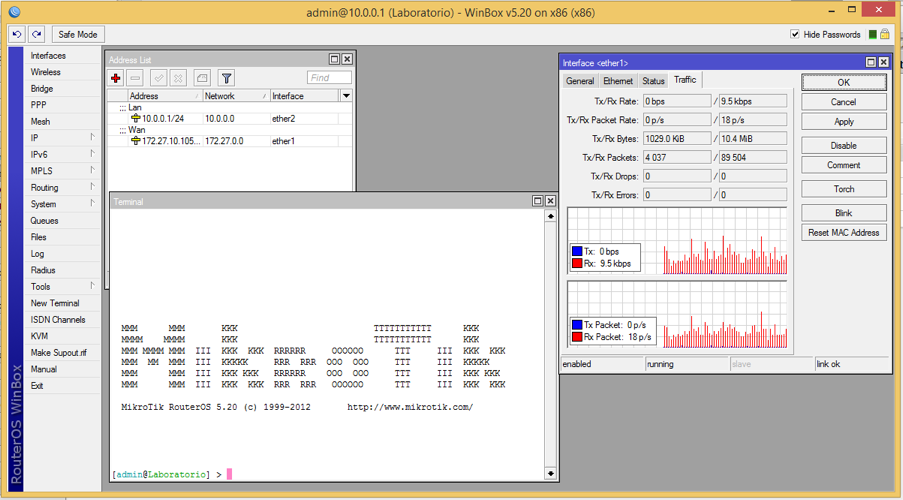
\includegraphics[scale = .5]{./figuras/figura025.png}
\caption{RouterOS}
\label{routeros}
\end{center}
\end{figure}

El Mikrotik RouterOS es un sistema operativo basado en el Kernel V3.5.5 de Linux y es muy estable, la facilidad de acceso a las m�ltiples configuraciones depender� del tipo de licencia a la que tengamos acceso con nuestro RouterBOARD. La licencia que este establecida en nuestro mainboard no tiene fecha de expiraci�n, pero si un tiempo de duraci�n en la que se podr� tener acceso a una nueva actualizaci�n.\cite{routeros:2010}

\section{Winbox.}
Winbox es un programa ejecutable en Windows, en Linux y Mac OSX por medio de WINE, que me permite acceder a las m�ltiples configuraciones de mi mainboard desde mi PC por medio de un entorno amigable. Es un software liviano que se lo puede descargar de la p�gina Mikrotik\cite{winbox:down} 
\begin{figure}[H]
\begin{center}
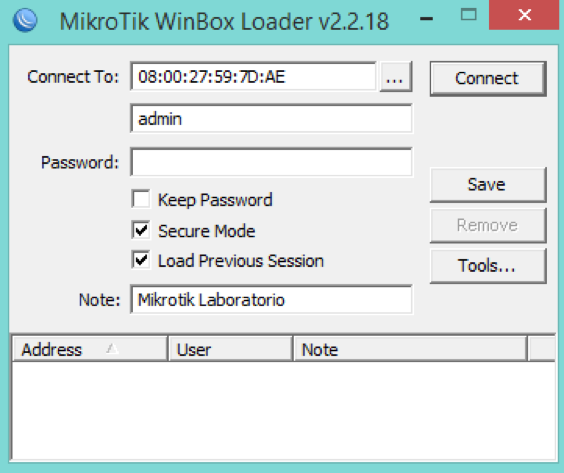
\includegraphics[scale = .5]{./figuras/figura026.png}
\caption{Winbox}
\label{winbox}
\end{center}
\end{figure}
Conectamos nuestro RouterBoard  a nuestra m�quina y le damos escanear en el bot�n ``...'' y nos mostrara todos los RouterBoard conectados.
Se selecciona el equipo con el usuario por defecto es \textit{admin} sin contrase�a

\begin{figure}[H]
\begin{center}
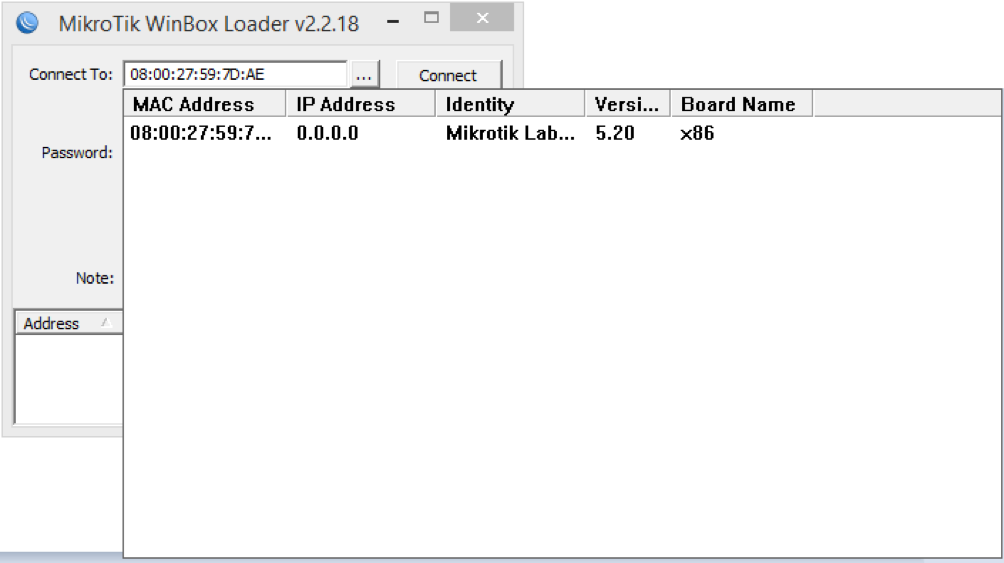
\includegraphics[scale = .5]{./figuras/figura027.png}
\caption{Escaneo de Router con Winbox}
\label{Escaneo}
\end{center}
\end{figure}
Una vez dentro del RouterBoard se selecciona: \textbf{New Terminal} y digitando \textit{``system reset''} para que vuelva a sus configuraciones de f�brica y evitar alg�n problema por otras configuraciones que pueden estar dentro del Router.
\begin{figure}[H]
\begin{center}
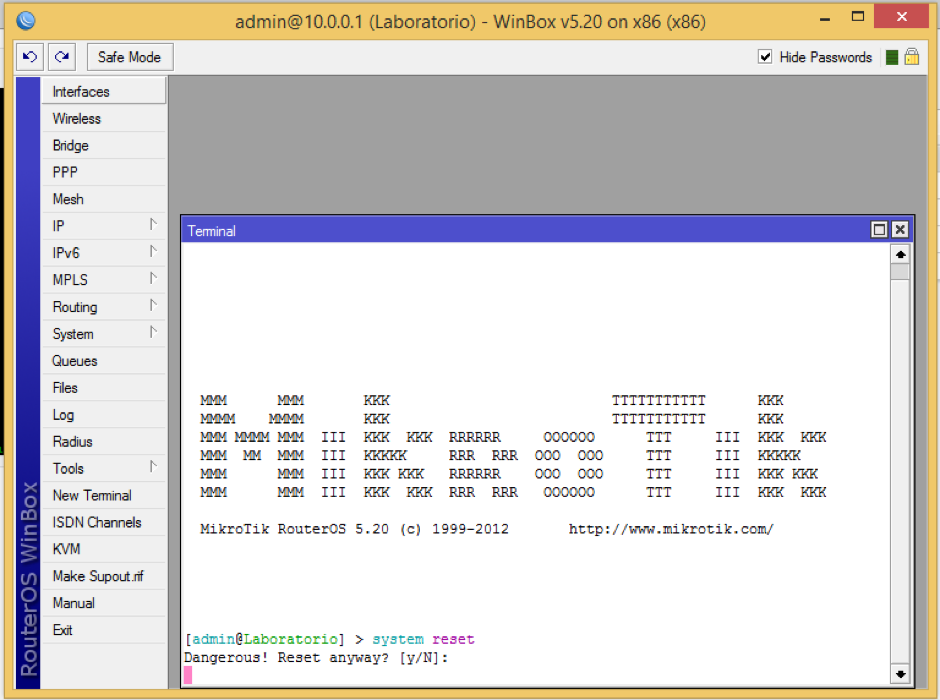
\includegraphics[scale = .5]{./figuras/figura028.png}
\caption{Reset RouterOS}
\label{resetrouter}
\end{center}
\end{figure}

Una vez que el RouterBoard reinicie, se accede v�a WinBox, para ver como quedo la configuraci�n.
\begin{figure}[H]
\begin{center}
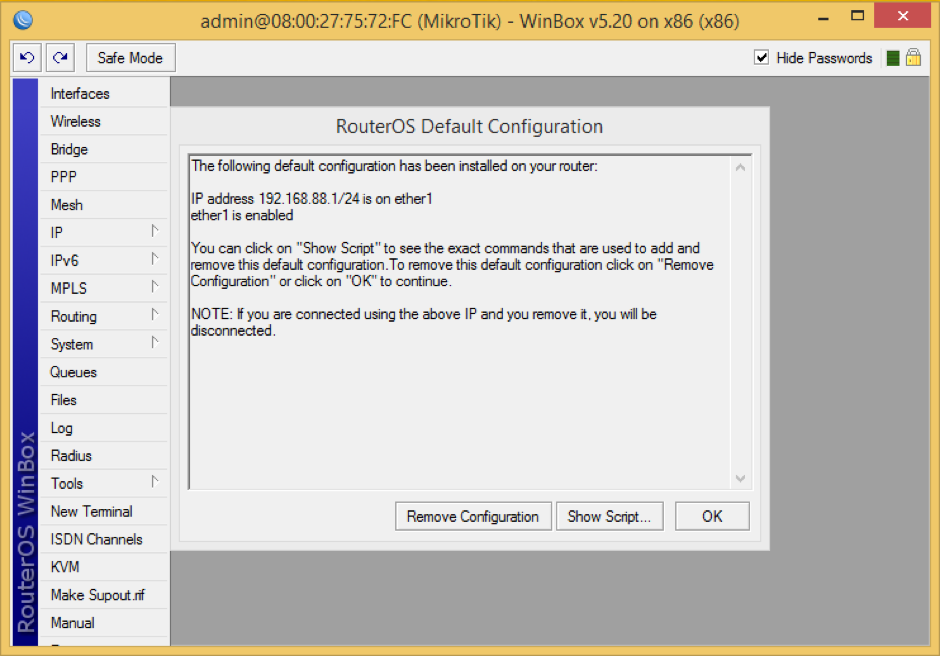
\includegraphics[scale = .5]{./figuras/figura029.png}
\caption{Remover Configuraciones}
\label{removerconfig}
\end{center}
\end{figure}

\section{Configuraci�n IP.}

Las IP (Internet Protocol) son muy importantes en cada uno de los enlaces ya que por medio de ellas se establecer� la comunicaci�n el enlace.
Para asignar una direcci�n IP a una interfaz tenemos que. \\
Escoger el men� \textbf{IP} $\rightarrow$  \textbf{Address}  $\rightarrow$ \textcolor{red}{\textbf{+}}\\
\begin{figure}[H]
\begin{center}
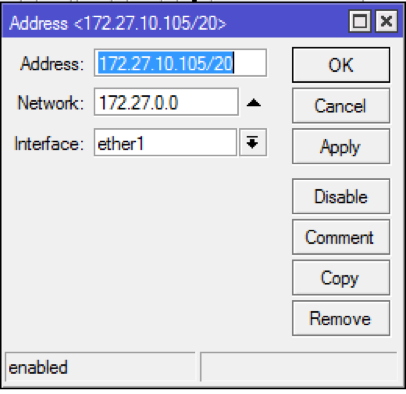
\includegraphics[scale = .5]{./figuras/figura030.png}
\caption{Configura IP WAN}
\label{ipwan}
\end{center}
\end{figure}
Escoger el men� \textbf{IP} $\rightarrow$  \textbf{Address}  $\rightarrow$ \textcolor{red}{\textbf{+}}\\
\begin{figure}[H]
\begin{center}
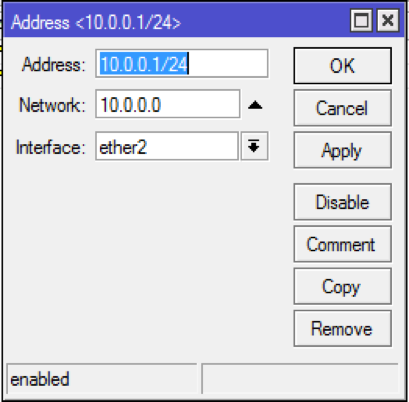
\includegraphics[scale = .5]{./figuras/figura031.png}
\caption{Configurar IP LAN}
\label{iplan}
\end{center}
\end{figure}
Escoger el men� \textbf{IP} $\rightarrow$  \textbf{Address}\\
\begin{figure}[H]
\begin{center}
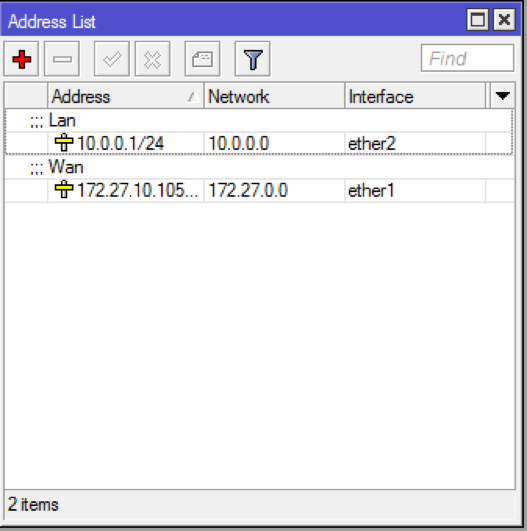
\includegraphics[scale = .5]{./figuras/figura032.png}
\caption{Address List}
\label{addresslist}
\end{center}
\end{figure}
Escoger el men� \textbf{IP} $\rightarrow$  \textbf{Routes}\\
\begin{figure}[H]
\begin{center}
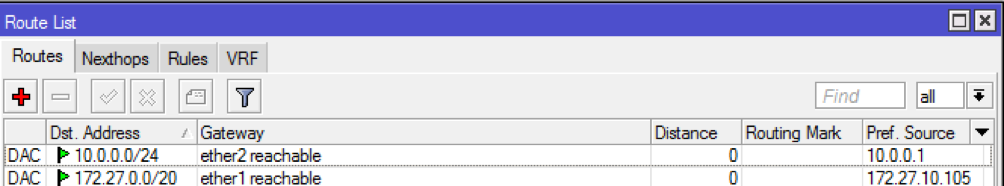
\includegraphics[scale = .5]{./figuras/figura033.png}
\caption{Puertas de Enlaces}
\label{routelist}
\end{center}
\end{figure}
Escoger el men� \textbf{IP} $\rightarrow$  \textbf{Routes} $\rightarrow$ \textcolor{red}{\textbf{+}}\\
\begin{figure}[H]
\begin{center}
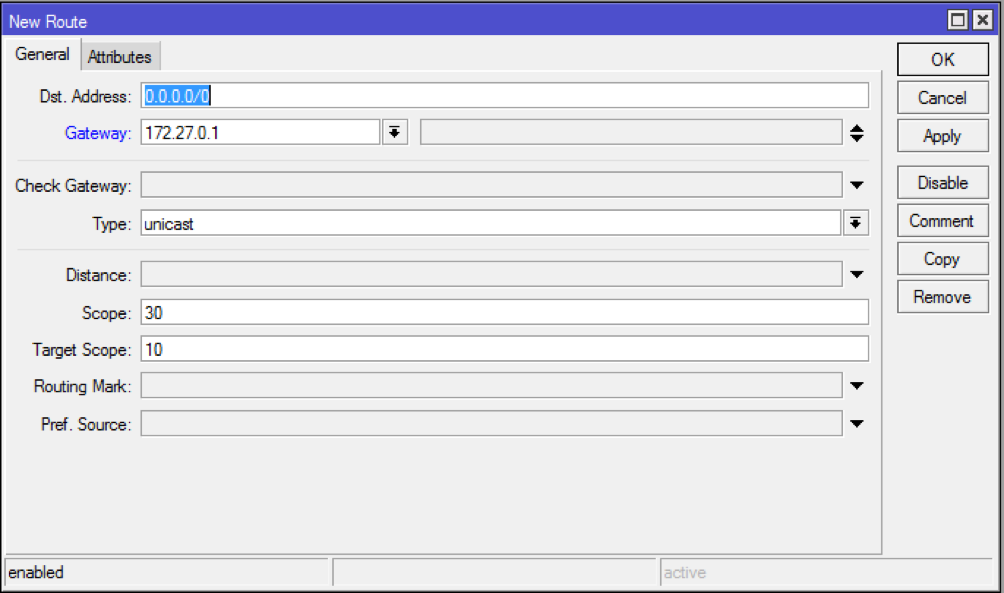
\includegraphics[scale = .5]{./figuras/figura034.png}
\caption{Puerta de enlace predeterminada}
\label{default-route}
\end{center}
\end{figure}
Escoger el men� \textbf{IP} $\rightarrow$  \textbf{Routes}\\
\begin{figure}[H]
\begin{center}
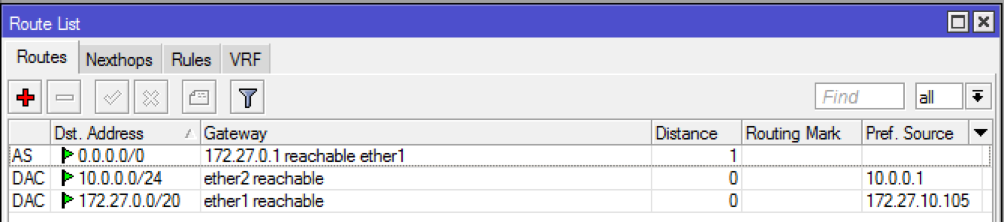
\includegraphics[scale = .5]{./figuras/figura035.png}
\caption{Listado de puertas de enlace}
\label{list-route}
\end{center}
\end{figure}

Escoger el men� \textbf{IP} $\rightarrow$  \textbf{DNS}\\
\begin{figure}[H]
\begin{center}
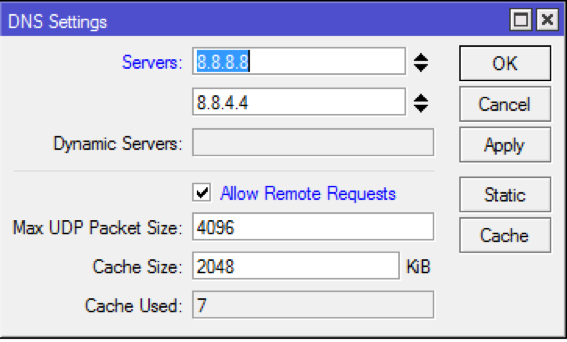
\includegraphics[scale = .5]{./figuras/figura036.png}
\caption{DNS}
\label{fig:dns}
\end{center}
\end{figure}

Escoger el men� \textbf{New Terminal} $\rightarrow$  \textbf{ping google.com}\\
\begin{figure}[H]
\begin{center}
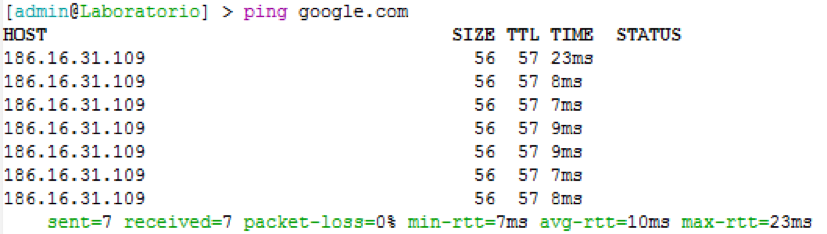
\includegraphics[scale = .5]{./figuras/figura037.png}
\caption{Prueba de ping}
\label{test-ping}
\end{center}
\end{figure}

Escoger el men� \textbf{IP} $\rightarrow$  \textbf{Firewall} $\rightarrow$ \textcolor{red}{\textbf{+}}\\
\begin{figure}[H]
\begin{center}
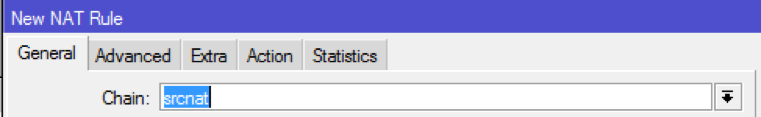
\includegraphics[scale = .5]{./figuras/figura038.png}
\caption{Firewall - General}
\label{firewall-general}
\end{center}
\end{figure}


Escoger el men� \textbf{IP} $\rightarrow$  \textbf{Firewall} \\
\begin{figure}[H]
\begin{center}
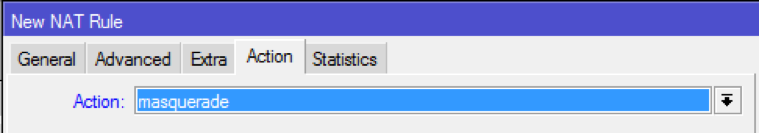
\includegraphics[scale = .5]{./figuras/figura039.png}
\caption{Firewall -Action}
\label{firewall-action}
\end{center}
\end{figure}

Escoger el men� \textbf{IP} $\rightarrow$  \textbf{Firewall} \\
\begin{figure}[H]
\begin{center}
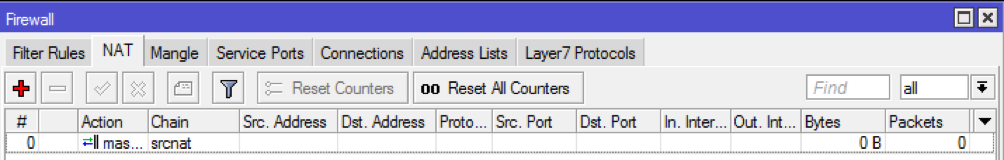
\includegraphics[scale = .5]{./figuras/figura040.png}
\caption{Lista reglas Nat}
\label{firewall-nat}
\end{center}
\end{figure}

Escoger el men� \textbf{Inicio} $\rightarrow$  \textbf{Ejecutar} $\rightarrow$  \textbf{cmd}\\
\begin{figure}[H]
\begin{center}
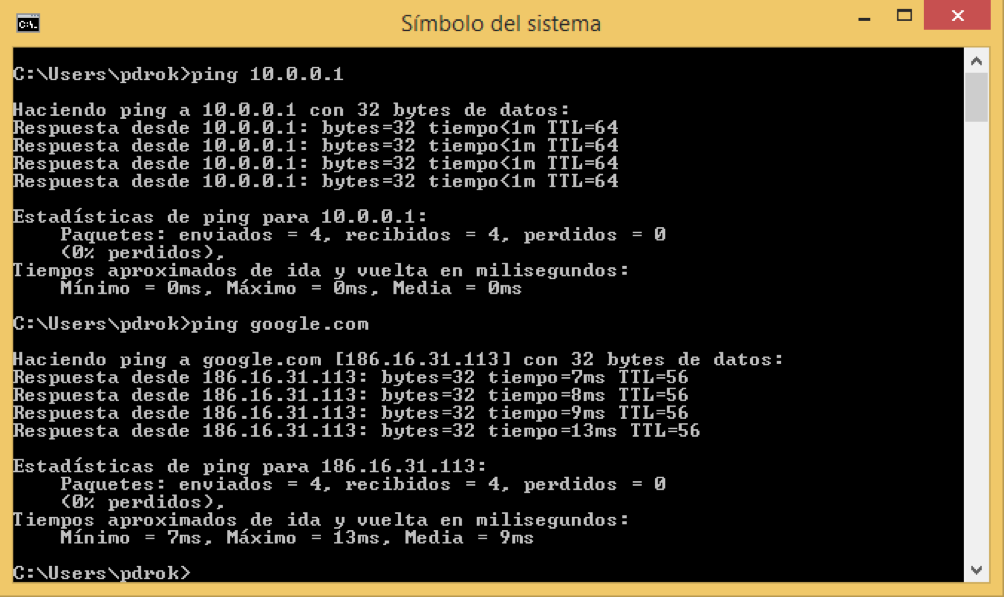
\includegraphics[scale = .5]{./figuras/figura041.png}
\caption{Prueba de ping}
\label{prueba-ping-cmd}
\end{center}
\end{figure}



\section{Telnet}
Telnet s�lo sirve para acceder en modo terminal, es decir, sin gr�ficos, pero es una herramienta muy �til para arreglar fallos a distancia, sin necesidad de estar f�sicamente en el mismo sitio que la m�quina que los ten�a. Tambi�n se usaba para consultar datos a distancia, como datos personales en m�quinas accesibles por red, informaci�n bibliogr�fica, etc.\cite{protocolo:telnet} 

\begin{figure}[H]
\begin{center}
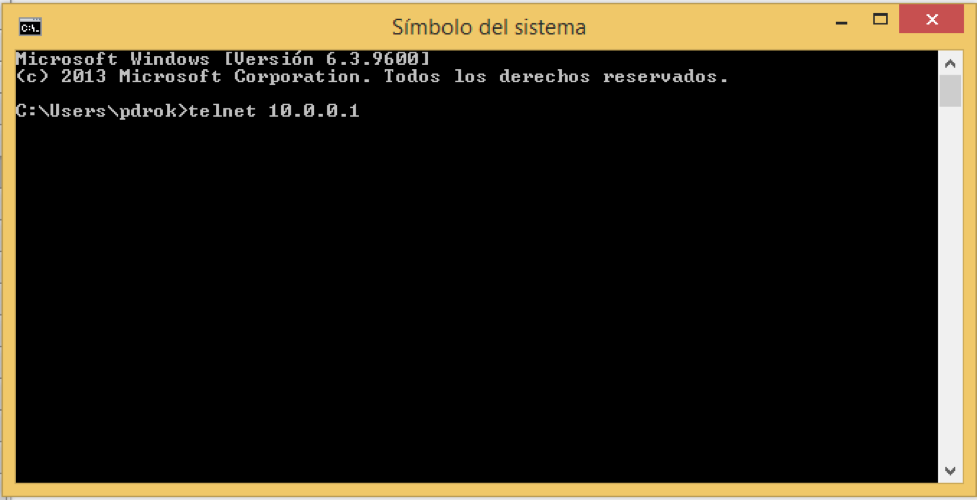
\includegraphics[scale = .5]{./figuras/figura042.png}
\caption{Acceso v�a Telnet}
\label{acceso-via-telnet}
\end{center}
\end{figure}

\begin{figure}[H]
\begin{center}
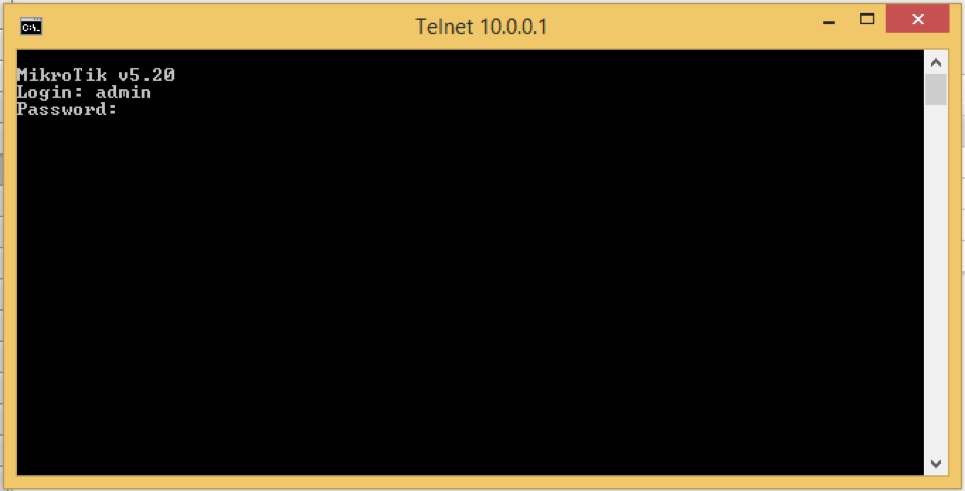
\includegraphics[scale = .5]{./figuras/figura043.png}
\caption{Credenciales v�a telnet}
\label{credenciales-via-telnet}
\end{center}
\end{figure}

\begin{figure}[H]
\begin{center}
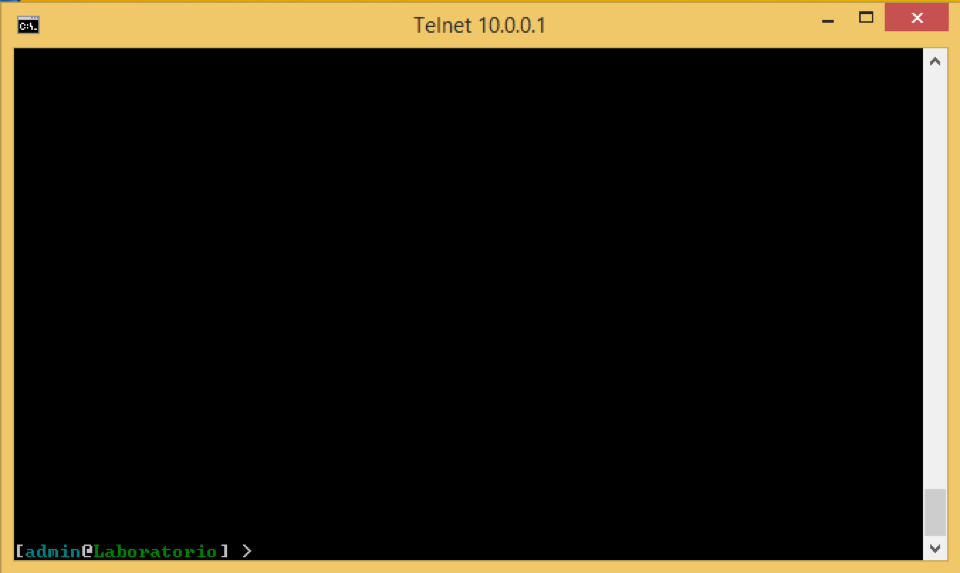
\includegraphics[scale = .5]{./figuras/figura044.png}
\caption{Entorno Telnet}
\label{entorno-telnet}
\end{center}
\end{figure}


\section{Webbox}
Es una manera de controlar y monitorear el Mikrotik RouterOS por medio de una navegador Web sin la necesidad de utilizar herramientas adicionales
\begin{figure}[H]
\begin{center}
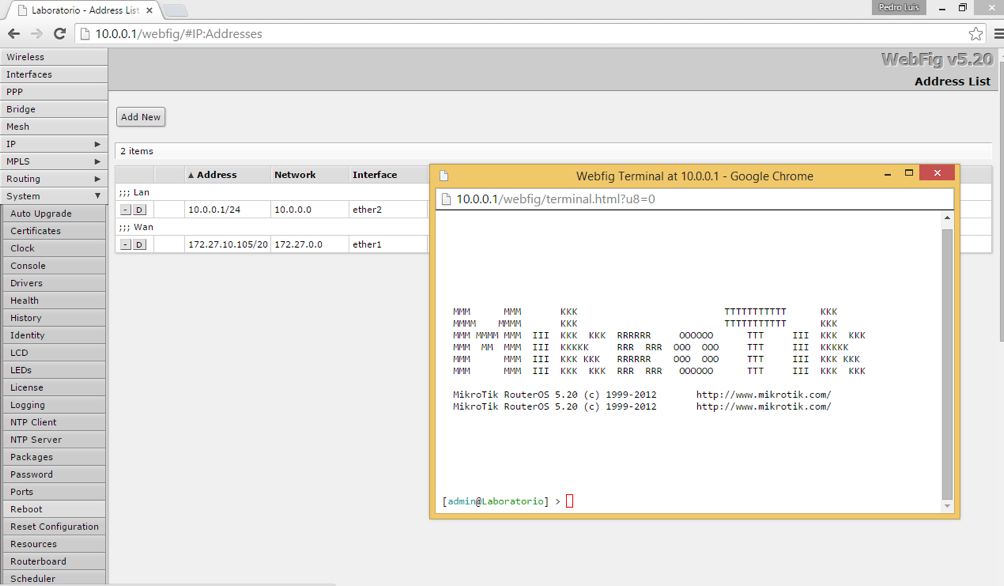
\includegraphics[scale = .8]{./figuras/figura045.png}
\caption{Webbox}
\label{webbox}
\end{center}
\end{figure}




\section{SSH}
\Gls{ssh} es un protocolo que facilita las comunicaciones seguras entre dos sistemas usando una arquitectura cliente/servidor y que permite a los usuarios conectarse a un host remotamente. A diferencia de otros protocolos de comunicaci�n remota tales como \Gls{ftp} o Gls{telnet}, SSH encripta la sesi�n de conexi�n, haciendo imposible que alguien pueda obtener contrase�as no encriptadas.\\

SSH est� dise�ado para reemplazar los m�todos m�s viejos y menos seguros para registrarse remotamente en otro sistema a trav�s de la shell de comando, tales como telnet o rsh \cite{protocolo:ssh}

\begin{figure}
\centering
\begin{tabular}{cc}
\subfloat[Putty]{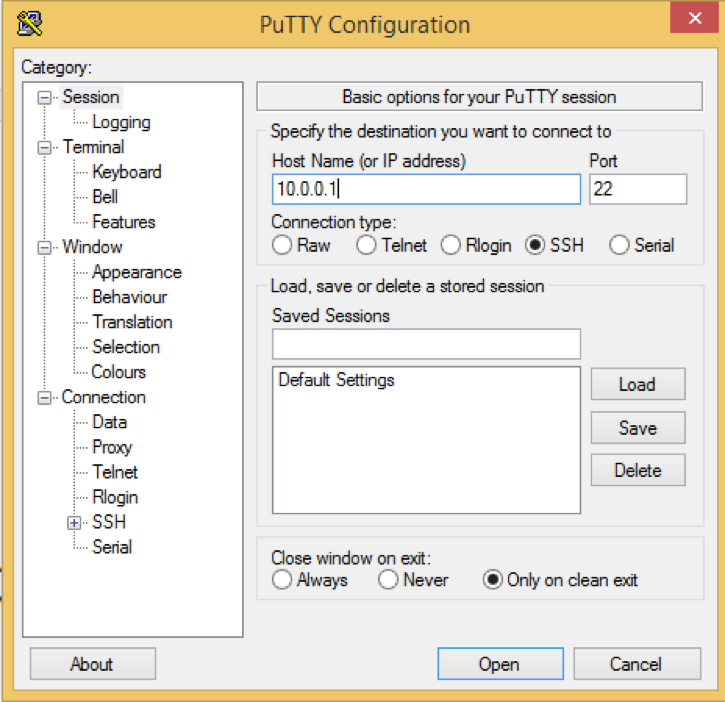
\includegraphics[scale = .5]{./figuras/figura046.png}} &
\subfloat[Autenticaci�n]{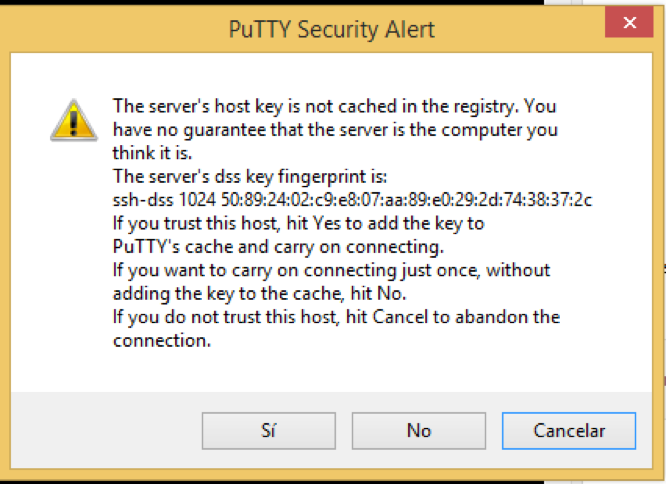
\includegraphics[scale = .5]{./figuras/figura047.png}}\\
\end{tabular}
\caption{Putty - Autenticaci�n}
\end{figure}

\begin{figure}[H]
\begin{center}
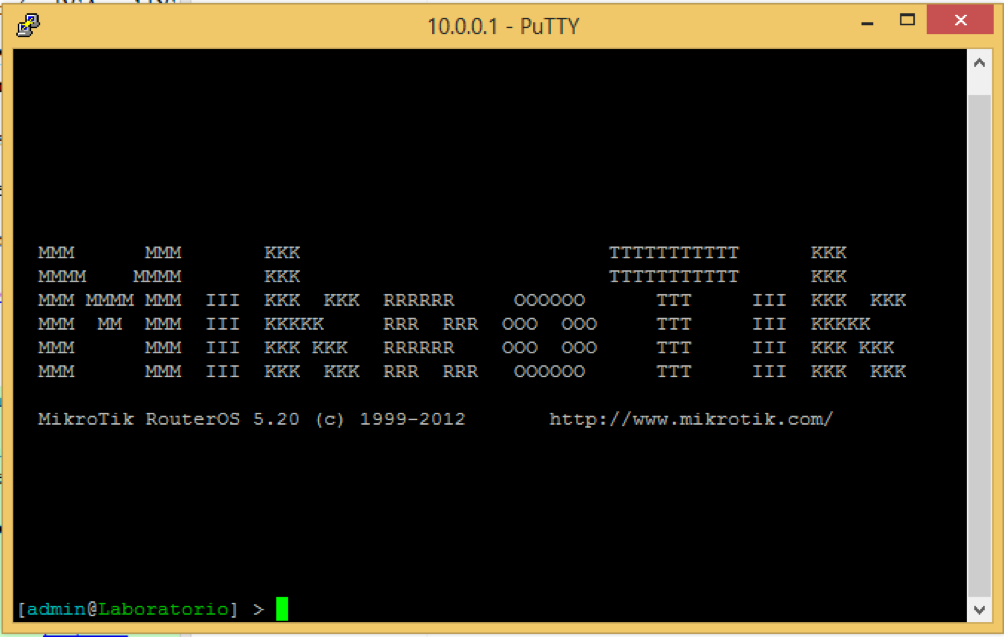
\includegraphics[scale = .5]{./figuras/figura048.png}
\caption{Entorno de trabajo SSH}
\label{entorno-ssh}
\end{center}
\end{figure}

\section{Radio Mobile}
Es un programa de simulaci�n de radiopropagaci�n gratuito desarrollado por Roger Coud� para predecir el comportamiento de sistemas radio, simular radioenlaces y representar el �rea de cobertura de una red de radiocomunicaciones, entre otras funciones. El software trabaja en el rango de frecuencias entre 20 MHz y 20 GHz y est� basado en el modelo de propagaci�n \Gls{itm} o modelo Longley-Rice. Utiliza datos de elevaci�n del terreno que se descargan gratuitamente de Internet para crear mapas virtuales del �rea de inter�s, vistas estereosc�picas, vistas en 3-D y animaciones de vuelo. Los datos de elevaci�n se pueden obtener de diversas fuentes, entre ellas del proyecto de la NASA que provee datos de altitud con una precisi�n de 3 segundos de arco (100m).\cite{radio:mobile}


\begin{figure}[H]
\begin{center}
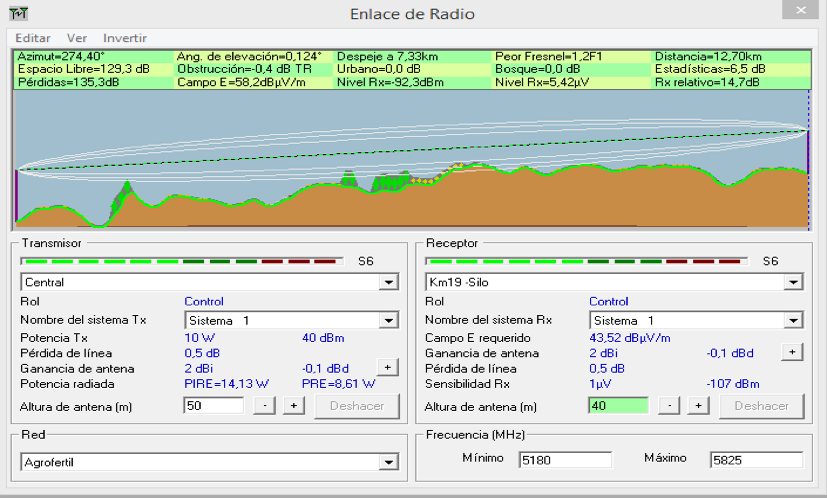
\includegraphics[scale = .8]{./figuras/figura049.png}
\caption{Radio Mobile, Enlace de Radio}
\label{rmobile-enlace-radio}
\end{center}
\end{figure}

\begin{figure}[H]
\begin{center}
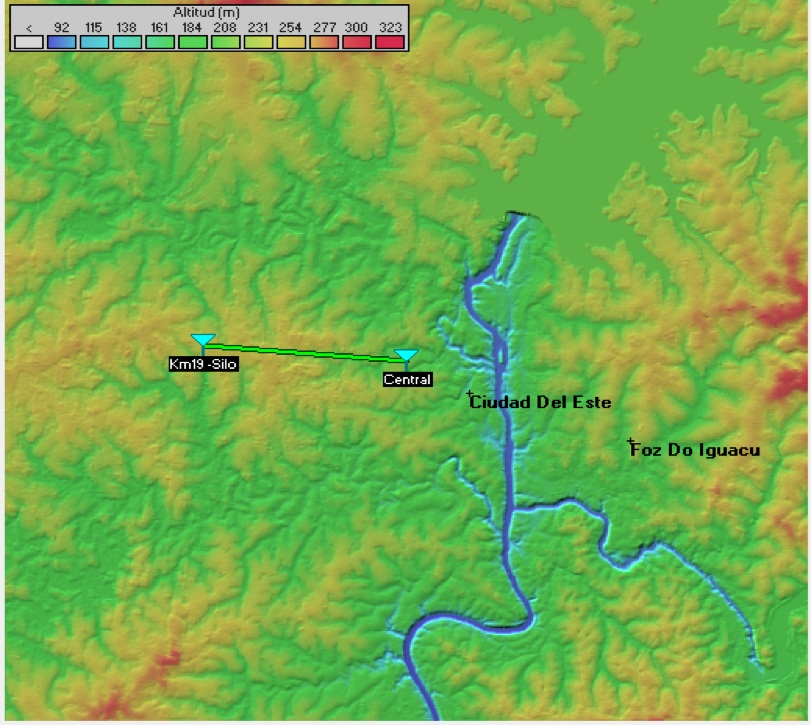
\includegraphics[scale = .8]{./figuras/figura050.png}
\caption{Vista con Radio Mobile}
\label{vista-radiomobile}
\end{center}
\end{figure}

\section{Google Earth}
Es un programa inform�tico que muestra un globo virtual que permite visualizar m�ltiple cartograf�a, con base en la fotograf�a satelital. El programa fue creado bajo el nombre de EarthViewer 3D por la compa��a Keyhole Inc, financiada por la Agencia Central de Inteligencia. La compa��a fue comprada por Google en 2004 absorbiendo la aplicaci�n.\\
El mapa de Google Earth est� compuesto por una superposici�n de im�genes obtenidas por im�genes satelitales, fotograf�as a�reas, informaci�n geogr�fica proveniente de modelos de datos SIG de todo el mundo y modelos creados por computadora. El programa est� disponible en varias licencias, pero la versi�n gratuita es la m�s popular, disponible para dispositivos m�viles, tabletas y computadoras personales.\\
La primera versi�n de Google Earth fue lanzada en 2005 y actualmente est� disponible en PC para Windows, Mac y Linux. Google Earth tambi�n est� disponible como plugin para visualizarse desde el navegador web. En 2013 Google Earth se hab�a convertido en el programa m�s popular para visualizar cartograf�a, con m�s de mil millones de descargas.\\

Muchos usuarios utilizan la aplicaci�n para a�adir sus propios datos, haci�ndolos disponibles mediante varias fuentes, tales como el Bulletin Board Systems o blogs. Google Earth es capaz de mostrar diferentes capas de imagen encima de la base y es tambi�n un cliente v�lido para un Web Map Service. Google Earth soporta datos geoespaciales tridimensionales mediante los archivos \gls{kml} \cite{google:earth}

\begin{figure}[H]
\begin{center}
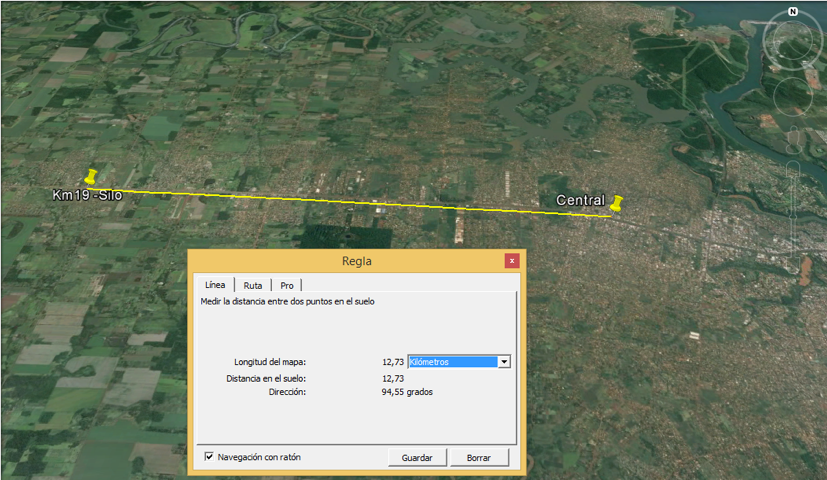
\includegraphics[scale = .8]{./figuras/figura051.png}
\caption{Vista con Google Earth}
\label{vista-googleearth}
\end{center}
\end{figure}



\fancyhead{}
\fancyfoot{}


\lhead{Realizar un radio enlace y t�nel redundante}

\chapter{Procedimientos generales para la instalaci�n de los enlaces}

Para que todo se entienda mejor se proceder� a una demostraci�n bastante sencilla que se ira indicando paso a paso.
\begin{figure}[H]
\begin{center}
\includegraphics[scale = .8]{./figuras/figura052.png}
\caption{Escenario para la Simulaci�n}
\label{escenario-simulacion}
\end{center}
\end{figure}

\begin{figure}[H]
\begin{center}
\includegraphics[scale = .7]{./figuras/figura053.png}
\caption{Escenario ya en limpio}
\label{escenario-limpio}
\end{center}
\end{figure}

\section{Equipos a ser utilizados}
\begin{figure}[H]
\begin{center}
\includegraphics[scale = .8]{./figuras/figura054.png}
\caption{Prueba de funcionamiento de los equipos}
\label{funcionamiento-equipos}
\end{center}
\end{figure}


\begin{figure}[H]
\begin{center}
\includegraphics[scale = .5]{./figuras/figura055.png}
\caption{MK4 y MK3}
\label{mk4-mk3}
\end{center}
\end{figure}


\begin{figure}[H]
\begin{center}
\includegraphics[scale = .5]{./figuras/figura056.png}
\caption{MK2 y MK1}
\label{mk2-mk1}
\end{center}
\end{figure}


\begin{figure}[H]
\begin{center}
\includegraphics[scale = .5]{./figuras/figura057.png}
\caption{Notebook Central}
\label{notebook-central}
\end{center}
\end{figure}


\begin{figure}[H]
\begin{center}
\includegraphics[scale = .5]{./figuras/figura058.png}
\caption{Maquina Sucursal 1}
\label{maquina-sucursal-1}
\end{center}
\end{figure}

\section{Configuraci�n de radios}
\subsection{Mikrotik RouterOS - enlaces punto - punto.}
Para establecer la comunicaci�n en un enlace inal�mbrico punto - puntos generalmente la topolog�a que se utiliza es la de \gls{ap} - Station. Este tipo de configuraci�n se lo hace en el modo de operaci�n de cada mainboard que forma parte del enlace.\\
Antes de iniciar con la configuraci�n respectiva de cada equipo es importante se�alar que existen algunos par�metros que se deben tomar en consideraci�n para garantizar la conexi�n del enlace; entre estos par�metros se encuentra: el \Gls{ssid} de la red, seguridad WEP, la banda de operaci�n y la frecuencia de trabajo (�nicamente en el AP, ya que la estaci�n trabajara? en la frecuencia del AP al que se conecte.)

\subsection{Configuraci�n AP}

Una vez inicializada nuestra consola de Winbox, accedemos al men� Interfaces, el mismo que nos presentara la ventana Interface List que me presentara? los diferentes puertos Ethernet e inal�mbricos de los que disponemos.
\begin{figure}[H]
\begin{center}
\includegraphics[scale = .5]{./figuras/figura059.png}
\caption{Escaneo de Routers}
\label{escaneo-routers}
\end{center}
\end{figure}

\begin{figure}[H]
\begin{center}
\includegraphics[scale = .5]{./figuras/figura060.png}
\caption{Reseteo de configuraciones}
\label{reseteo-configuraciones}
\end{center}
\end{figure}

\begin{figure}[H]
\begin{center}
\includegraphics[scale = .5]{./figuras/figura061.png}
\caption{Remover configuraci�n}
\label{remover-configuracion-61}
\end{center}
\end{figure}


Ya que la configuraci�n es inal�mbrica procedemos a la configuraci�n de nuestra tarjeta wlan1en el Men� Wireless wlan1 A continuaci�n describiremos �nicamente los par�metros m�s importantes a configurar para un enlace AP.
\subsubsection{General}
\textbf{Name:} Permite cambiar el nombre de la interface en la que encontramos.\\
\textbf{Type:} Muestra el tipo de chip que utiliza la mini PcI.\\
\textbf{\Gls{mtu}:} Expresa el tama�o en byte de la unidad de datos m�s grande que puede enviarse usando un Protocolo de Internet.
\subsubsection{Wireless}
\textbf{Mode:} Designa el modo de funcionamiento de la interfaz en este caso AP Bridge.\\
\textbf{Band:} hace referencia al rango de frecuencia sobre el cual se va a trabajar. Frecuencia: Especifica el canal permanente sobre el cual se va a traficar la informaci�n.\\
\textbf{SSID:} es un c�digo incluido en todos los paquetes que se trafican por una red inal�mbrica, para identificarlos como parte de la misma.\\
\textbf{Security Profile:} Es un c�digo Hexadecimal creado con el fin de evitar que usuarios sin una autorizaci�n formen parte de la red.\\
\textbf{Antena Mode:} Ya que las tarjetas miniPCI dispones para dos conectores, en el momento que este se conecta en el principal (main), colocamos como antena a, si por el contrario decidimos conectar al otro puerto (aux), el modo sera? antena b.\\
\textbf{Antena Gain:} Ganancia de la antena externa que estemos utilizando (en dBi).
\textbf{Tx-Power:} En la opci�n de potencia podremos controlar la potencia de salida de las miniPCI, (en dBi).
\begin{figure}[H]
\begin{center}
\includegraphics[scale = .5]{./figuras/figura062.png}
\caption{Interface Wireless disponible}
\label{interface-wire-dispo}
\end{center}
\end{figure}

\begin{figure}[H]
\begin{center}
\includegraphics[scale = .5]{./figuras/figura063.png}
\caption{Configurar AP}
\label{configurar-ap}
\end{center}
\end{figure}

\begin{figure}[H]
\begin{center}
\includegraphics[scale = .5]{./figuras/figura064.png}
\caption{Habilitar Bridge - WDS}
\label{bridge-wds}
\end{center}
\end{figure}
 
\begin{figure}[H]
\begin{center}
\includegraphics[scale = .5]{./figuras/figura065.png}
\caption{Equipos ya conectado}
\label{equipo-conectado}
\end{center}
\end{figure}
 

\subsubsection{Configuraci�n Bridge.}
El crear un bridge me permitir� comunicar dos o m�s interfaces dentro de una misma tarjera; para ello seguimos los siguientes pasos:\\

Escoger el men� \textbf{Brige} $\rightarrow$ \textcolor{red}{\textbf{+}}\\
\begin{figure}[H]
\begin{center}
\includegraphics[scale = .5]{./figuras/figura066.png}
\caption{Nombre Bridge}
\label{nombre-bridge}
\end{center}
\end{figure}
 Escoger el men� \textbf{Brige} $\rightarrow$ \textbf{ports} $\rightarrow$ \textcolor{red}{\textbf{+}}\\
\begin{figure}[H]
\begin{center}
\includegraphics[scale = .5]{./figuras/figura067.png}
\caption{Agregar Interface al Bridge}
\label{agregar-interface-bridge-67}
\end{center}
\end{figure}
 
 Escoger el men� \textbf{Brige} $\rightarrow$ \textbf{ports}\\
\begin{figure}[H]
\begin{center}
\includegraphics[scale = .5]{./figuras/figura068.png}
\caption{Lista de Puerto del Bridge}
\label{lista-puerto-bridge-68}
\end{center}
\end{figure}
 
 Escoger el men� \textbf{New Terminal} $\rightarrow$ \textbf{ping 10.0.0.3}
\begin{figure}[H]
\begin{center}
\includegraphics[scale = .5]{./figuras/figura069.png}
\caption{Prueba de ping al MK3}
\label{prueba-ping-mk3}
\end{center}
\end{figure}
 
 Escoger el men� \textbf{Tools} $\rightarrow$ \textbf{Bandwidth Test}
\begin{figure}[H]
\begin{center}
\includegraphics[scale = .5]{./figuras/figura070.png}
\caption{Prueba de Ancho de banda}
\label{prueba-ancho-banda}
\end{center}
\end{figure}
 
\begin{figure}[H]
\begin{center}
\includegraphics[scale = .5]{./figuras/figura071.png}
\caption{Una vez conectado, ya muesta al escanear todas las radios}
\label{conectado-muesta-escanear-radios}
\end{center}
\end{figure}
  Escoger el men� \textbf{Inicio} $\rightarrow$ \textbf{ejecutar} $\rightarrow$ \textbf{cmd}
\begin{figure}[H]
\begin{center}
\includegraphics[scale = .5]{./figuras/figura072.png}
\caption{Prueba de ping desde la Red Central}
\label{prueba-ping-red-central}
\end{center}
\end{figure}
 
\subsection{Configuraci�n Estaci�n.}
La configuraci�n de nuestra estaci�n es mucho m�s sencilla ya que como estaci�n tendremos que configurar �nicamente los siguientes par�metros:\\

\textbf{General}\\
\textbf{Name:} Permite cambiar el nombre de la interface en la que os encontramos.\\\
\textbf{Type:} Muestra el tipo de chip que utiliza la mini PcI.MTU (unidad m�xima de transferencia): Expresa el tama�o en byte de la unidad de datos m�s grande que puede enviarse usando un Protocolo de Internet. \\
\textbf{Wireless}\\
\textbf{Mode:} Designa el modo de funcionamiento de la interfaz en este caso AP Bridge.\\
\textbf{Band:} hace referencia al rango de frecuencia sobre el cual se va a trabajar. 
\textbf{Frecuencia:} Especifica el canal permanente sobre el cual se va a traficar informaci�n dado por el AP al que se conecta.\\
\textbf{SSID:} Ya que la estaci�n pertenecer� a la misma red del AP, esta tendr� que utilizar el mismo SSID.\\
\textbf{Security Profile:} Al igual que con el SSID, la estaci�n debe tener la misma seguridad para comunicar los dos equipos.\\
\textbf{Antena Mode:} Ya que las targejas miniPCI dispones para dos conectores, en el momento que este se conecta en el principal (main), colocamos como antena a, si por el contrario decidimos conectar al otro puerto (aux), el modo ser� antena b.\\
\textbf{Antena Gain:} Ganancia de la antena externa que estemos utilizando (en dBi).\\
\textbf{Tx-Power:} En la opci�n de potencia podremos controlar la potencia de salida de las miniPCI, (en dBi).\\
Escoger el men� \textbf{New Terminal} $\rightarrow$  \textbf{system reset-configuration} 
\begin{figure}[H]
\begin{center}
\includegraphics[scale = .5]{./figuras/figura073.png}
\caption{Reestablecer Configuraciones MK3}
\label{reestablecer-configuraciones-mk3}
\end{center}
\end{figure}
 Escoger el men� \textbf{Remove Configuration} 
\begin{figure}[H]
\begin{center}
\includegraphics[scale = .5]{./figuras/figura074.png}
\caption{Remover configuraciones}
\label{remover-configuraciones-74}
\end{center}
\end{figure}
 Escoger el men� \textbf{Brige} $\rightarrow$ \textcolor{red}{\textbf{+}}\\
\begin{figure}[H]
\begin{center}
\includegraphics[scale = .5]{./figuras/figura075.png}
\caption{Crear Bridge}
\label{crear-bridge}
\end{center}
\end{figure}
 Escoger el men� \textbf{Bridge} $\rightarrow$  \textbf{Ports} 
\begin{figure}[H]
\begin{center}
\includegraphics[scale = .5]{./figuras/figura076.png}
\caption{Lista de interfaces en el Bridge}
\label{lista-interfaces-bridge}
\end{center}
\end{figure}
 Escoger el men� \textbf{IP} $\rightarrow$  \textbf{Address}  $\rightarrow$ \textcolor{red}{\textbf{+}}\\
\begin{figure}[H]
\begin{center}
\includegraphics[scale = .5]{./figuras/figura077.png}
\caption{Configurar IP}
\label{configurar-ip}
\end{center}
\end{figure}
 Escoger el men� \textbf{Wireless} 
\begin{figure}[H]
\begin{center}
\includegraphics[scale = .5]{./figuras/figura078.png}
\caption{Lista Interfaces Wireless disponibles}
\label{lista-interfaces-wireless-disponibles}
\end{center}
\end{figure}
 Escoger el men� \textbf{Wireless} $\rightarrow$  \textbf{wlan1}  $\rightarrow$ \textbf{Wireless}\\
\begin{figure}[H]
\begin{center}
\includegraphics[scale = .5]{./figuras/figura079.png}
\caption{Configurar Wireless Station}
\label{configurar-wireless-station}
\end{center}
\end{figure}
% Bridge y WDS escribir algo sobre estos dos bichos.. 
Escoger el men� \textbf{Wireless} $\rightarrow$  \textbf{wlan1}  $\rightarrow$ \textbf{WDS}\\
\begin{figure}[H]
\begin{center}
\includegraphics[scale = .5]{./figuras/figura080.png}
\caption{Configura interface en la Bridge y WDS}
\label{configura-interface-bridge-wds}
\end{center}
\end{figure}
 
\section{Configuraci�n de VPN}

La especificaci�n para PPTP fue publicada por el RFC 2637\cite{rfc:2637}, aunque no ha sido ratificada como est�ndar por el IETF.\\

Point-To-Point Tunneling Protocol (\Gls{pptp}) permite el intercambio seguro de datos de un cliente a un servidor formando una Red Privada Virtual (VPN, por el anglicismo Virtual Private Network), basado en una red de trabajo v�a \Gls{tcp/ip}. El punto fuerte del PPTP es su habilidad para proveer en la demanda, multi-protocolo soporte existiendo una infraestructura de �rea de trabajo, como INTERNET. Esta habilidad permitir� a una compa��a usar Internet para establecer una red privada virtual (VPN) sin el gasto de una l�nea alquilada.
 
Escoger el men� \textbf{New Terminal} $\rightarrow$  \textbf{system-reset} \\
\subsection{Configuraci�n VPN Server} 
\begin{figure}[H]
\begin{center}
\includegraphics[scale = .5]{./figuras/figura081.png}
\caption{Restaurar configuraciones MK1}
\label{restaurar-configuraciones-mk1}
\end{center}
\end{figure}

 Escoger el men� \textbf{Mac Address} $\rightarrow$  \textbf{Connect}\\
\begin{figure}[H]
\begin{center}
\includegraphics[scale = .5]{./figuras/figura082.png}
\caption{Winbox con el MK1 ya con las configuraciones de fabrica}
\label{Winbox-mk1-configuraciones-fabrica}
\end{center}
\end{figure}
 
Escoger el men� \textbf{Remove Configuration} \\
\begin{figure}[H]
\begin{center}
\includegraphics[scale = .5]{./figuras/figura083.png}
\caption{Remover configuraciones}
\label{remover-configuraciones-83}
\end{center}
\end{figure}

Escoger el men� \textbf{IP} $\rightarrow$  \textbf{Address}  $\rightarrow$ \textcolor{red}{\textbf{+}}\\
\begin{figure}[H]
\begin{center}
\includegraphics[scale = .5]{./figuras/figura084.png}
\caption{Configurar IP}
\label{configurar-ip-84}
\end{center}
\end{figure}

 Escoger el men� \textbf{Wireless} $\rightarrow$  \textbf{wlan1}  $\rightarrow$ \textbf{Wireless}\\
\begin{figure}[H]
\begin{center}
\includegraphics[scale = .5]{./figuras/figura085.png}
\caption{Conectar al WIFI del Celular}
\label{conectar-wifi-celular-85}
\end{center}
\end{figure}

 Escoger el men� \textbf{Wireless} $\rightarrow$  \textbf{Security Profiles}  $\rightarrow$ \textcolor{red}{\textbf{+}}\\
\begin{figure}[H]
\begin{center}
\includegraphics[scale = .5]{./figuras/figura086.png}
\caption{Configuraciones de Seguridad del WIFI}
\label{confi-seguridad-wifi-86}
\end{center}
\end{figure}
 
\begin{figure}[H]
\begin{center}
\includegraphics[scale = .3]{./figuras/figura102.png}
\caption{MK1 y MK4 conectado al Celular}
\label{mk-conectado-cel}
\end{center}
\end{figure}
 

Habilitamos el PPTP Server, para eso nos vamos a la opcion de /PPP Interface; acemos clic e el boton PPTP Server hacemos click en Enabled y en default Profile escogemos default-encryptation. Aplicamos, de esta forma estamos hablilitando al servidor para que permita coneccione PPTP.

Escoger el men� \textbf{PPP} $\rightarrow$  \textbf{PPTP-Server} \\
\begin{figure}[H]
\begin{center}
\includegraphics[scale = .5]{./figuras/figura087.png}
\caption{Habilitar Server PPTP}
\label{habilitar-server-pptp}
\end{center}
\end{figure}
 
Ahora agregamos nuestros Clientes VPN, Para eso nos vamos a la pesta�a Secrets, y agregamos los usuarios que sean necesarios.\\

\textbf{Name:} Nombre de Usuario VPN\\
\textbf{Password:} Contrase�a del Usuario VPN\\
\textbf{Service:} Tipo de Protocolo que usara el cliente para su coneccion con el servidor.\\
\textbf{Profile:} Perfil de encryptacion \\
\textbf{Local Address:} Direcci�n IP del equipo anfitri�n, del router local (La IP de puerta de enlace de nuestra LAN anfitri�n.)\\
\textbf{Remote address:} Direccion IP con la cual el equipo cliente se identificara en nuestra re LAN.\\

Escoger el men� \textbf{ppp} $\rightarrow$  \textbf{Secret}  $\rightarrow$ \textcolor{red}{\textbf{+}}\\
\begin{figure}[H]
\begin{center}
\includegraphics[scale = .5]{./figuras/figura088.png}
\caption{Crear usuario para T�nel por medio del Enlace}
\label{usuario-tunel-enlace}
\end{center}
\end{figure}

Escoger el men� \textbf{ppp} $\rightarrow$  \textbf{Secret}  $\rightarrow$ \textcolor{red}{\textbf{+}}\\
\begin{figure}[H]
\begin{center}
\includegraphics[scale = .5]{./figuras/figura089.png}
\caption{Crear usuario para el T�nel por medio de Internet}
\label{usuario-tunel-internet}
\end{center}
\end{figure}

 Escoger el men� \textbf{PPP} $\rightarrow$  \textbf{Interfaces}\\
\begin{figure}[H]
\begin{center}
\includegraphics[scale = .5]{./figuras/figura090.png}
\caption{T�nel ya online}
\label{tunel-online}
\end{center}
\end{figure}

 Escoger el men� \textbf{IP} $\rightarrow$  \textbf{Address List}\\
\begin{figure}[H]
\begin{center}
\includegraphics[scale = .5]{./figuras/figura091.png}
\caption{Listado de IP del MK1}
\label{listado-ip-mk1}
\end{center}
\end{figure} 

 \subsection{Configuraci�n VPN Cliente}

Escoger el men� \textbf{New Terminal} $\rightarrow$ \textbf{system reset-configuration}\\
\begin{figure}[H]
\begin{center}
\includegraphics[scale = .5]{./figuras/figura092.png}
\caption{Remover configuraciones}
\label{remover-configuraciones}
\end{center}
\end{figure}
Escoger el men� \textbf{Remove Configuration} \\
\begin{figure}[H]
\begin{center}
\includegraphics[scale = .5]{./figuras/figura093.png}
\caption{Remover configuraciones por defecto}
\label{remover-configuraciones-defecto}
\end{center}
\end{figure}

Escoger el men� \textbf{Wireless} $\rightarrow$  \textbf{wlan1} $\rightarrow$ \textbf{Wireless}\\
\begin{figure}[H]
\begin{center}
\includegraphics[scale = .5]{./figuras/figura094.png}
\caption{configurar WIFI}
\label{configurar-wifi}
\end{center}
\end{figure}

Escoger el men� \textbf{Wireless} $\rightarrow$  \textbf{Security Profiles}  $\rightarrow$ \textcolor{red}{\textbf{+}}\\

\begin{figure}[H]
\begin{center}
\includegraphics[scale = .5]{./figuras/figura095.png}
\caption{Perfil de seguridad del WIFI}
\label{perfil-seguridad-wifi}
\end{center}
\end{figure}

 Escoger el men� \textbf{IP} $\rightarrow$  \textbf{Address List}  
\begin{figure}[H]
\begin{center}
\includegraphics[scale = .5]{./figuras/figura096.png}

\caption{Lista de IP configurado MK4}
\label{lista-ip-configurado-mk4}
\end{center}
\end{figure}
 Escoger el men� \textbf{ppp} $\rightarrow$ \\
\begin{figure}[H]
\begin{center}
\includegraphics[scale = .5]{./figuras/figura097.png}
\caption{Lista de Discadores Clientes}
\label{lista-discadores-conectado}
\end{center}
\end{figure}

\lhead{Configurar VPN - Discadores}
\textbf{Configurar Discadores:}\\
\textbf{Connect To:} Direcci�n IP con la cual el equipo cliente se identificara en nuestra re LAN\\
\textbf{Name:} Nombre de Usuario VPN\\
\textbf{Password:} Contrase�a del Usuario VPN\\
\textbf{Profile:} Perfil de encryptacion
Escoger el men� \textbf{PPP} $\rightarrow$  \textbf{Secret}  $\rightarrow$ \textcolor{red}{\textbf{+}}\\
\begin{figure}[H]
\begin{center}
\includegraphics[scale = .5]{./figuras/figura098.png}
\caption{Datos Discador Cliente por Internet}
\label{discador-cliente-internet}
\end{center}
\end{figure}
 Escoger el men� \textbf{ppp} $\rightarrow$  \textbf{Secret}  $\rightarrow$ \textcolor{red}{\textbf{+}}\\
\begin{figure}[H]
\begin{center}
\includegraphics[scale = .5]{./figuras/figura099.png}
\caption{Datos Discador Cliente VPN por Enlace}
\label{discador-cliente-enlace}
\end{center}
\end{figure}
 Escoger el men� \textbf{IP} $\rightarrow$  \textbf{Routes} $\rightarrow$ \textcolor{red}{\textbf{+}}\\
\begin{figure}[H]
\begin{center}
\includegraphics[scale = .5]{./figuras/figura100.png}
\caption{Configuraciones de Puertas de enlace}
\label{config-puerta-enlace}
\end{center}
\end{figure}

Escoger el men� \textbf{Inicio} $\rightarrow$  \textbf{ejecutar}  $\rightarrow$ \textbf{cmd}\\

\begin{figure}[H]
\begin{center}
\includegraphics[scale = .5]{./figuras/figura101.png}
\caption{Prueba de \gls{traceroute} desde la maquina Sucursal 1}
\label{prueba-tracert}
\end{center}
\end{figure}

\fancyhead{}
\fancyfoot{}


\lhead{Conclusi�n y recomendaciones}

\chapter{Conclusi�n}


El modelo de infraestructura que responde de manera m�s pr�ctica y eficiente para la centralizaci�n de datos es utilizando VPN a trav�s de radio enlaces y reforzando con enlaces de internet.
Los equipos hardware y software utilizados para la implementaci�n de la centralizaci�n de datos a trav�s de VPN responden de manera eficiente al costo beneficio, la marca Mikrotik es mucha m�s barata que otras tecnolog�as de su competencia como Cisco. Presenta la robustez necesaria para los radios enlaces.
La cantidad de recursos humanos necesarios y el orden de desarrollo del trabajo para la implementaci�n de la centralizaci�n de datos a trav�s de VPN fueron evaluados y demostraron ventajas en costos beneficios. Antes se necesitaba si o si una persona de TI por cada local, con la implementaci�n de la centralizaci�n ya no existe esa necesidad. Adem�s, se economiza los costos de la locomoci�n.
Las recomendaciones para tener una seguridad m�nima en la centralizaci�n de los datos a trav�s de VPN es la administraci�n eficiente de las mismas, ya que todos los equipos re�nen las condiciones necesarias para la implementaci�n de la seguridad.
Las 21 filiales anexadas a la central y la administraci�n de la mismas de manera remota genera una gran econom�a a la empresa y es un modelo replicable a otras empresas que buscan mejor infraestructura para la administraci�n de su informaci�n.
Se recomienda la instalaci�n de enlaces con equipamientos RouterBoard por la practicidad, robustez y econom�a.

\section{Trabajos Futuros}

Esta seccio?n discute las limitaciones de este trabajo, y en base a eso se formularon posibles opciones de futura investigacio?n para mejorar el disen?o y enfoque de disen?o propuesto en este trabajo.\\ 
Enfocar en la seguridad de la red en distintos puntos.\\
Monitorear los equipos por medio de email y sms, con software como Zabbix, Cati o Whatsup Gold.\\
Configurar para que los equipos puedan actualizar sus configuraciones por medio de ftp.\\
Realizar pruebas de comparacion con equipos de otras marcas, como Ubiquiti Networks.\\

\backmatter

\cleardoublepage
\addcontentsline{toc}{chapter}{Glosario}
\printglossary

\cleardoublepage
%\addcontentsline{toc}{chapter}{Anexos}
\fancyhead{}
\fancyfoot{}


\lhead{Anexo A.}
%\rhead{\today}
%\rfoot{\thepage}

\chapter{Anexo A.}

\section{Configuraciones del MK1}
\begin{verbatim}
# mar/02/2016 19:28:43 by RouterOS 6.15
# software id = SLWX-PKH2
/ip firewall nat
 add action=masquerade chain=srcnat
/system identity
 set name=MK1
/ip address
 add address=192.168.0.1/24 interface=ether5 network=192.168.0.0
 add address=10.0.0.1/24 interface=ether2 network=10.0.0.0
/ppp secret
 add local-address=11.0.0.1 name=vpn1 password=vpn1 \
 remote-address=11.0.0.2 routes="192.168.1.0/24 11.0.0.2 1"
 add local-address=12.0.0.1 name=vpn2 password=vpn2 \
 remote-address=12.0.0.2 routes="192.168.1.0/24 12.0.0.2 1"
/interface pptp-server server
 set enabled=yes max-mru=1460 max-mtu=1460
/interface wireless security-profiles
 set [ find default=yes ] supplicant-identity=MikroTik
 add authentication-types=wpa-psk,wpa2-psk eap-methods="" \
 management-protection=allowed mode=dynamic-keys name=profile1 \
 supplicant-identity="" wpa-pre-shared-key="123.123.!" \
 wpa2-pre-shared-key="123.123.!"
/user
 add comment="system default user" group=full name=admin
/interface wireless security-profiles
 set [ find default=yes ] supplicant-identity=MikroTik
 add authentication-types=wpa-psk,wpa2-psk eap-methods="" \
 management-protection=allowed mode=dynamic-keys name=profile1 \
 supplicant-identity="" wpa-pre-shared-key="123.123.!" \
 wpa2-pre-shared-key="123.123.!"
/interface wireless
 set [ find default-name=wlan1 ] disabled=no l2mtu=2290 \
 security-profile=profile1 ssid=Azureos
\end{verbatim}
\section{Configuraciones del MK2}
\begin{verbatim}
# mar/02/2016 19:08:54 by RouterOS 6.32.1
# software id = U9B0-UXDW
#
/system identity
 set name=MK2
 
/interface bridge
 add name=bridge1
 
/interface bridge port
 add bridge=bridge1 interface=ether1
 add bridge=bridge1 interface=ether2
 add bridge=bridge1 interface=wlan1
/interface bridge port
 add bridge=bridge1 interface=ether1
 add bridge=bridge1 interface=ether2
 add bridge=bridge1 interface=wlan1
 
/ip address
 add address=10.0.0.2/24 interface=bridge1 network=10.0.0.0
/interface wireless security-profiles
 set [ find default=yes ] supplicant-identity=MikroTik
 
/user
 add comment="system default user" group=full name=admin
/interface wireless
 set [ find default-name=wlan1 ] disabled=no l2mtu=1600 \
 mode=ap-bridge ssid=Link01 wds-default-bridge=bridge1 \
 wds-mode=dynamic
 
/interface wireless security-profiles
 set [ find default=yes ] supplicant-identity=MikroTik
\end{verbatim}
\section{Configuraciones del MK3}
\begin{verbatim}
# mar/02/2016 19:09:40 by RouterOS 5.26
# software id = IKF9-H3ZS
#
/system identity
 set name=MK3

/interface bridge
 add admin-mac=00:00:00:00:00:00 ageing-time=5m arp=enabled \
 auto-mac=yes disabled=no forward-delay=15s l2mtu=1522 \
 max-message-age=20s mtu=1500 name=bridge1 priority=0x8000 \
 protocol-mode=none transmit-hold-count=6
 
/interface bridge port
 add bridge=bridge1 disabled=no edge=auto external-fdb=auto \
 horizon=none interface=wlan1 path-cost=10 point-to-point=auto \
 priority=0x80
 add bridge=bridge1 disabled=no edge=auto external-fdb=auto \
 horizon=none interface=ether2 path-cost=10 point-to-point=auto \
 priority=0x80
 add bridge=bridge1 disabled=no edge=auto external-fdb=auto \
 horizon=none interface=ether3 path-cost=10 point-to-point=auto \
 priority=0x80
 add bridge=bridge1 disabled=no edge=auto external-fdb=auto \
 horizon=none interface=ether1 path-cost=10 point-to-point=auto \
 priority=0x80
 
/interface bridge settings
 set use-ip-firewall=no use-ip-firewall-for-pppoe=no \ 
 use-ip-firewall-for-vlan=no
/interface bridge port
 add bridge=bridge1 disabled=no edge=auto external-fdb=auto \
 horizon=none interface=wlan1 path-cost=10 point-to-point=auto \
 priority=0x80
 add bridge=bridge1 disabled=no edge=auto external-fdb=auto \
 horizon=none interface=ether2 path-cost=10 point-to-point=auto \
 priority=0x80
 add bridge=bridge1 disabled=no edge=auto external-fdb=auto \
 horizon=none interface=ether3 path-cost=10 point-to-point=auto \
 priority=0x80 
 add bridge=bridge1 disabled=no edge=auto external-fdb=auto \
 horizon=none interface=ether1 path-cost=10 point-to-point=auto \
 priority=0x80
 
/ip dns
 set allow-remote-requests=no cache-max-ttl=1w cache-size=2048KiB \
 max-udp-packet-size=4096 servers=""

/ip address
 add address=10.0.0.3/24 disabled=no interface=bridge1 \
 network=10.0.0.0
/interface pptp-server server
 set authentication=mschap1,mschap2 default-profile=default-\
 encryption enabled=no keepalive-timeout=30 max-mru=1460 max-\
 mtu=1460 mrru=disabled
 
/interface wireless security-profiles
 set [ find default=yes ] authentication-types="" eap-met\
 hods=passthrough group-ciphers=aes-ccm group-key-update=5m\
 interim-update=0s \
 management-protection=disabled management-protection-key=""\
 mode=none \
 name=default radius-eap-accounting=no radius-mac-accounting=no \
 radius-mac-authentication=no radius-mac-caching=disabled \
 radius-mac-format=XX:XX:XX:XX:XX:XX radius-mac-mode=as-username \
 static-algo-0=none static-algo-1=none static-algo-2=none static-\
 algo-3=none static-key-0="" static-key-1="" static-key-2="" \
 static-key-3=""static-sta-private-algo=none static-sta-private-\
 key="" static-transmit-key=key-0 supplicant-identity=MikroTik \
 tls-certificate=none tls-mode=no-certificates unicast-ciphers=\
 aes-ccm wpa-pre-shared-key="" wpa2-pre-shared-key=""

/user group
 set read name=read policy="local,telnet,ssh,reboot,read\
 ,test,winbox,password,web,sniff,sensitive,api,!ftp,!write\
 ,!policy" skin=default
 set write name=write policy="local,telnet,ssh,reboot,read,\
 write,test,winbox,password,web,sniff,sensitive,api,!ftp,!po\
 licy" skin=default set full name=full policy="local,telnet,\
 ssh,ftp,reboot,read,write,policy,test,winbox,password,web,sn\
 iff,sensitive,api" skin=default
 
/user
 add address="" comment="system default user" disabled=no \
 group=full name=admin
/user aaa
 set accounting=yes default-group=read exclude-groups="" \
 interim-update=0s use-radius=no

/interface wireless security-profiles
 set [ find default=yes ] authentication-types="" eap-\
 methods=passthrough group-ciphers=aes-ccm group-key-\
 update=5m interim-update=0s management-protection=disa\
 bled management-protection-key="" mode=none name=default \
 radius-eap-accounting=no radius-mac-accounting=no radius-\
 mac-authentication=no radius-mac-caching=disabled radius-\
 mac-format=XX:XX:XX:XX:XX:XX radius-mac-mode=as-username \
 static-algo-0=none static-algo-1=none static-algo-2=none \
 static-algo-3=none static-key-0="" static-key-1="" static\
 -key-2="" static-key-3="" static-sta-private-algo=none \
 static-sta-private-key="" static-transmit-key=key-0 suppl\
 icant-identity=MikroTik tls-certificate=none tls-mode=no-\
 certificates unicast-ciphers=aes-ccm wpa-pre-shared-key=\
 "" wpa2-pre-shared-key=""
/interface wireless
 set 0 adaptive-noise-immunity=none allow-sharedkey=no \
 antenna-gain=0 antenna-mode=ant-a area="" arp=enabled \
 band=5ghz-a basic-rates-a/g=6Mbps bridge-mode=enabled \
 burst-time=disabled channel-width=20mhz compression=\
 no country=no_country_set default-ap-tx-limit=0 \
 default-authentication=yes default-client-tx-limit=0 \
 default-forwarding=yes dfs-mode=none disable-running-\
 check=no disabled=no disconnect-timeout=3s distance=\
 dynamic frame-lifetime=0 frequency=5180 frequency-mode=\
 manual-txpower frequency-offset=0 hide-ssid=no hw-fragmen\
 tation-threshold=disabled hw-protection-mode=none hw-prote\
 ction-threshold=0 hw-retries=7 l2mtu=2290 mac-address=\
 00:15:6D:6C:7D:72 max-station-count=2007 mode=station-wds \
 mtu=1500 multicast-helper=default name=wlan1 noise-floor-\
 threshold=default nv2-cell-radius=30 nv2-noise-floor-\
 offset=default nv2-preshared-key="" nv2-qos=default nv2-\
 queue-count=2 nv2-security=disabled on-fail-retry-time=100ms \
 periodic-calibration\
 =default periodic-calibration-interval=60 preamble-mode=both \
 proprietary-extensions=post-2.9.25 radio-name=00156D6C7D72 \
 rate-selection=advanced rate-set=default scan-list=default \
 security-profile=default ssid=Link01 station-bridge-clone-mac=\
 00:00:00:00:00:00 supported-rates-a/g=\
 6Mbps,9Mbps,12Mbps,18Mbps,24Mbps,36Mbps,48Mbps,54Mbps tdma-period\
 -size=2 tx-power-mode=default update-stats-interval=disabled wds-\
 cost-range=50-150 wds-default-bridge=bridge1 wds-default-cost=100\ 
 wds-ignore-ssid=no wds-mode=dynamic wireless-protocol=unspecified \
 wmm-support=disabled
/interface wireless manual-tx-power-table
 set wlan1 manual-tx-powers="1Mbps:17,2Mbps:17,5.5Mbps:17,\
 11Mbps:17,6Mbps:17,9Mbps:17,12Mbps:17,18Mbps:17,24Mbps:17,\
 36Mbps:17,48Mbps:17,54Mbps:17,HT20-0:17,HT20-1:17,HT20-2:17,\
 HT20-3:17,HT20-4:17,HT20-5:17,HT20-6:17,HT20-7:17,HT40-0:17,\
 HT40-1:17,HT40-2:17,HT40-3:17,HT40-4:17,HT40-5:17,HT40-6:17,\
 HT40-7:17"
/interface wireless nstreme
 set wlan1 disable-csma=no enable-nstreme=no enable-polling=yes \
 framer-limit=3200 framer-policy=none
/interface wireless align
 set active-mode=yes audio-max=-20 audio-min=-100 audio-monitor=\
 00:00:00:00:00:00 filter-mac=00:00:00:00:00:00 frame-size=300 \
 frames-per-second=25 receive-all=no ssid-all=no
/interface wireless sniffer
 set channel-time=200ms file-limit=10 file-name="" \
 memory-limit=10 multiple-channels=no only-headers=no \
 receive-errors=no streaming-enabled=no streaming-max-rate=0 \
 streaming-server=0.0.0.0
/interface wireless snooper
 set channel-time=200ms multiple-channels=yes receive-errors=no
\end{verbatim}
\section{Configuraciones del MK4}
\begin{verbatim}
# mar/02/2016 19:04:59 by RouterOS 6.23
# software id = K9T9-N0KR
#
/system identity
 set name=MK4
/ip firewall nat
add action=masquerade chain=srcnat

/ip address
 add address=10.0.0.4/24 interface=ether2 network=10.0.0.0
 add address=192.168.1.1/24 interface=ether3 network=192.168.1.0

/ip route
 add check-gateway=ping distance=1 dst-address=192.168.0.0/24 \
 gateway=11.0.0.1
 add check-gateway=ping distance=2 dst-address=192.168.0.0/24 \
 gateway=12.0.0.1

/interface pptp-client
 add add-default-route=no allow=pap,chap,mschap1,mschap2 \
 connect-to=10.0.0.1 dial-on-demand=no disabled=no \
 keepalive-timeout=60 max-mru=1460 max-mtu=1460 mrru=1600 \
 name=vpn1 password=vpn1 profile=default-encryption user=vpn1

 add add-default-route=no allow=pap,chap,mschap1,mschap2 \
 connect-to=192.168.43.90 dial-on-demand=no disabled=no \
 keepalive-timeout=60 max-mru=1460 max-mtu=1460 mrru=1600 \
 name=vpn2 password=vpn2 profile=default-encryption user=vpn2

/interface wireless security-profiles
 set [ find default=yes ] supplicant-identity=MikroTik
 add authentication-types=wpa-psk,wpa2-psk eap-methods="" \
 management-protection=allowed mode=dynamic-keys name=profile1 \
 supplicant-identity="" wpa-pre-shared-key="123.123.!" \
 wpa2-pre-shared-key="123.123.!"

/user
 add comment="system default user" group=full name=admin

/interface wireless security-profiles
 set [ find default=yes ] supplicant-identity=MikroTik
 add authentication-types=wpa-psk,wpa2-psk eap-methods="" \
 management-protection=allowed mode=dynamic-keys \
 name=profile1 supplicant-identity="" \
 wpa-pre-shared-key="123.123.!"wpa2-pre-shared-key="123.123.!"
/interface wireless
 set [ find default-name=wlan1 ] band=2ghz-b/g disabled=no \
 frequency=auto l2mtu=2290 security-profile=profile1 \
 ssid=Azureos

\end{verbatim}

\cleardoublepage
\addcontentsline{toc}{chapter}{Referencias bibliogr\'aficas}

\bibliographystyle{IEEEtran}
\bibliography{test}
\end{document}
